%% (Master) Thesis template
% Template version used: v1.4
%
% Largely adapted from Adrian Nievergelt's template for the ADPS
% (lecture notes) project.


%% We use the memoir class because it offers a many easy to use features.
\documentclass[11pt,a4paper,titlepage]{memoir}

%% Packages
%% ========

%% LaTeX Font encoding -- DO NOT CHANGE
\usepackage[OT1]{fontenc}

%% Babel provides support for languages.  'english' uses British
%% English hyphenation and text snippets like "Figure" and
%% "Theorem". Use the option 'ngerman' if your document is in German.
%% Use 'american' for American English.  Note that if you change this,
%% the next LaTeX run may show spurious errors.  Simply run it again.
%% If they persist, remove the .aux file and try again.
\usepackage[english]{babel}

%% Input encoding 'utf8'. In some cases you might need 'utf8x' for
%% extra symbols. Not all editors, especially on Windows, are UTF-8
%% capable, so you may want to use 'latin1' instead.
\usepackage[utf8]{inputenc}

%% This changes default fonts for both text and math mode to use Herman Zapfs
%% excellent Palatino font.  Do not change this.
\usepackage[sc]{mathpazo}

%% The AMS-LaTeX extensions for mathematical typesetting.  Do not
%% remove.
\usepackage{amsmath,amssymb,amsfonts,mathrsfs}

%% NTheorem is a reimplementation of the AMS Theorem package. This
%% will allow us to typeset theorems like examples, proofs and
%% similar.  Do not remove.
%% NOTE: Must be loaded AFTER amsmath, or the \qed placement will
%% break
\usepackage[amsmath,thmmarks]{ntheorem}

%% LaTeX' own graphics handling
\usepackage{graphicx}

%% We unfortunately need this for the Rules chapter.  Remove it
%% afterwards; or at least NEVER use its underlining features.
\usepackage{soul}

%% This allows you to add .pdf files. It is used to add the
%% declaration of originality.
\usepackage{pdfpages}

%% Some more packages that you may want to use.  Have a look at the
%% file, and consult the package docs for each.
%% See the TeXed file for more explanations

%% [OPT] Multi-rowed cells in tabulars
%\usepackage{multirow}

%% [REC] Intelligent cross reference package. This allows for nice
%% combined references that include the reference and a hint to where
%% to look for it.
\usepackage{varioref}

%% [OPT] Easily changeable quotes with \enquote{Text}
%\usepackage[german=swiss]{csquotes}

%% [REC] Format dates and time depending on locale
\usepackage{datetime}

%% [OPT] Provides a \cancel{} command to stroke through mathematics.
%\usepackage{cancel}

%% [NEED] This allows for additional typesetting tools in mathmode.
%% See its excellent documentation.
\usepackage{mathtools}

%% [ADV] Conditional commands
%\usepackage{ifthen}

%% [OPT] Manual large braces or other delimiters.
%\usepackage{bigdelim, bigstrut}

%% [REC] Alternate vector arrows. Use the command \vv{} to get scaled
%% vector arrows.


%% [NEED] Some extensions to tabulars and array environments.
\usepackage{array}

%% [OPT] Postscript support via pstricks graphics package. Very
%% diverse applications.
%\usepackage{pstricks,pst-all}

%% [?] This seems to allow us to define some additional counters.
%\usepackage{etex}

%% [ADV] XY-Pic to typeset some matrix-style graphics
%\usepackage[all]{xy}

%% [OPT] This is needed to generate an index at the end of the
%% document.
%\usepackage{makeidx}

%% [OPT] Fancy package for source code listings.  The template text
%% needs it for some LaTeX snippets; remove/adapt the \lstset when you
%% remove the template content.
\usepackage{listings}
\lstset{language=TeX,basicstyle={\normalfont\ttfamily}}

%% [REC] Fancy character protrusion.  Must be loaded after all fonts.
\usepackage[activate]{pdfcprot}

%% [REC] Nicer tables.  Read the excellent documentation.
\usepackage{booktabs}

%%Improt imaages
\usepackage{graphicx}

%% For pseudocode 
\usepackage[]{algorithm2e}

%% Symbols 
\usepackage{amssymb}
%\usepackage{ esint }
\usepackage{ upgreek }% can't include cause too many alphabet error 

\usepackage{todonotes}

%moving figures
\usepackage{float}

\usepackage{subcaption}

%better bold
\usepackage{bm}

%%% From bcfw paper 



%



%% Our layout configuration.  DO NOT CHANGE.
%% Memoir layout setup

%% NOTE: You are strongly advised not to change any of them unless you
%% know what you are doing.  These settings strongly interact in the
%% final look of the document.

% Dependencies
\usepackage{ETHlogo}

% Turn extra space before chapter headings off.
\setlength{\beforechapskip}{0pt}

\nonzeroparskip
\parindent=0pt
\defaultlists

% Chapter style redefinition
\makeatletter

\if@twoside
  \pagestyle{Ruled}
  \copypagestyle{chapter}{Ruled}
\else
  \pagestyle{ruled}
  \copypagestyle{chapter}{ruled}
\fi
\makeoddhead{chapter}{}{}{}
\makeevenhead{chapter}{}{}{}
\makeheadrule{chapter}{\textwidth}{0pt}
\copypagestyle{abstract}{empty}

\makechapterstyle{bianchimod}{%
  \chapterstyle{default}
  \renewcommand*{\chapnamefont}{\normalfont\Large\sffamily}
  \renewcommand*{\chapnumfont}{\normalfont\Large\sffamily}
  \renewcommand*{\printchaptername}{%
    \chapnamefont\centering\@chapapp}
  \renewcommand*{\printchapternum}{\chapnumfont {\thechapter}}
  \renewcommand*{\chaptitlefont}{\normalfont\huge\sffamily}
  \renewcommand*{\printchaptertitle}[1]{%
    \hrule\vskip\onelineskip \centering \chaptitlefont\textbf{\vphantom{gyM}##1}\par}
  \renewcommand*{\afterchaptertitle}{\vskip\onelineskip \hrule\vskip
    \afterchapskip}
  \renewcommand*{\printchapternonum}{%
    \vphantom{\chapnumfont {9}}\afterchapternum}}

% Use the newly defined style
\chapterstyle{bianchimod}

\setsecheadstyle{\Large\bfseries\sffamily}
\setsubsecheadstyle{\large\bfseries\sffamily}
\setsubsubsecheadstyle{\bfseries\sffamily}
\setparaheadstyle{\normalsize\bfseries\sffamily}
\setsubparaheadstyle{\normalsize\itshape\sffamily}
\setsubparaindent{0pt}

% Set captions to a more separated style for clearness
\captionnamefont{\sffamily\bfseries\footnotesize}
\captiontitlefont{\sffamily\footnotesize}
\setlength{\intextsep}{16pt}
\setlength{\belowcaptionskip}{1pt}

% Set section and TOC numbering depth to subsection
\setsecnumdepth{subsection}
\settocdepth{subsection}

%% Titlepage adjustments
\pretitle{\vspace{0pt plus 0.7fill}\begin{center}\HUGE\sffamily\bfseries}
\posttitle{\end{center}\par}
\preauthor{\par\begin{center}\let\and\\\Large\sffamily}
\postauthor{\end{center}}
\predate{\par\begin{center}\Large\sffamily}
\postdate{\end{center}}

\def\@advisors{}
\newcommand{\advisors}[1]{\def\@advisors{#1}}
\def\@department{}
\newcommand{\department}[1]{\def\@department{#1}}
\def\@thesistype{}
\newcommand{\thesistype}[1]{\def\@thesistype{#1}}

\renewcommand{\maketitlehooka}{\noindent\ETHlogo[2in]}

\renewcommand{\maketitlehookb}{\vspace{1in}%
  \par\begin{center}\Large\sffamily\@thesistype\end{center}}

\renewcommand{\maketitlehookd}{%
  \vfill\par
  \begin{flushright}
    \sffamily
    \@advisors\par
    \@department, ETH Z\"urich
  \end{flushright}
}

\checkandfixthelayout

\setlength{\droptitle}{-48pt}

\makeatother

% This defines how theorems should look. Best leave as is.
\theoremstyle{plain}
\setlength\theorempostskipamount{0pt}

%%% Local Variables:
%%% mode: latex
%%% TeX-master: "thesis"
%%% End:

%% Theorem environments.  You will have to adapt this for a German
%% thesis.
%% Theorem-like environments

%% This can be changed according to language. You can comment out the ones you
%% don't need.

\numberwithin{equation}{chapter}

%% German theorems
%\newtheorem{satz}{Satz}[chapter]
%\newtheorem{beispiel}[satz]{Beispiel}
%\newtheorem{bemerkung}[satz]{Bemerkung}
%\newtheorem{korrolar}[satz]{Korrolar}
%\newtheorem{definition}[satz]{Definition}
%\newtheorem{lemma}[satz]{Lemma}
%\newtheorem{proposition}[satz]{Proposition}

%% English variants
\newtheorem{theorem}{Theorem}[chapter]
\newtheorem{example}[theorem]{Example}
\newtheorem{remark}[theorem]{Remark}
\newtheorem{corollary}[theorem]{Corollary}
\newtheorem{definition}[theorem]{Definition}
\newtheorem{lemma}[theorem]{Lemma}
\newtheorem{proposition}[theorem]{Proposition}

%% Proof environment with a small square as a "qed" symbol
\theoremstyle{nonumberplain}
\theorembodyfont{\normalfont}
\theoremsymbol{\ensuremath{\square}}
\newtheorem{proof}{Proof}
%\newtheorem{beweis}{Beweis}

%% Helpful macros.
%% Custom commands
%% ===============

%% Special characters for number sets, e.g. real or complex numbers.
\newcommand{\C}{\mathbb{C}}
\newcommand{\K}{\mathbb{K}}
\newcommand{\N}{\mathbb{N}}
\newcommand{\Q}{\mathbb{Q}}
\newcommand{\R}{\mathbb{R}}
\newcommand{\Z}{\mathbb{Z}}
\newcommand{\X}{\mathbb{X}}

%% Fixed/scaling delimiter examples (see mathtools documentation)
\DeclarePairedDelimiter\abs{\lvert}{\rvert}
\DeclarePairedDelimiter\norm{\lVert}{\rVert}

%% Also set the alternate phi as default.
%\let\oldphi\phi
%\renewcommand{\phi}{\ensuremath{\varphi}}

\DeclareMathOperator*{\argmax}{arg\,max}
\DeclareMathOperator*{\argmin}{arg\,min}


%% Variables for my common symbols 

\newcommand{\error}{\upxi}
\newcommand{\xSpace}{\mathcal{X}}
\newcommand{\ySpace}{\mathcal{Y}_i}
\newcommand{\ySpaceNoI}{\mathcal{Y}}
\newcommand{\yVec}{\yVect}
\newcommand{\yVect}{\bm{y}}
\newcommand{\wv}{\weightVec}
\newcommand{\weightVec}{\weightVect}
\newcommand{\weightVect}{\bm{w}} %TODO this should be bold lowercase W but for some reason \boldsymbol cuases an error, maybe its cause of the BM package
\newcommand{\weightsmall}{\mathcal{w}}
\newcommand{\setOfVertecies} {\nu}
\newcommand{\setOfEdges}{\zeta}
\newcommand{\inputArgs}[1]{"#1"}
\newcommand{\jointFeatureMapAlone}{\psi}
\newcommand{\jointFeatureMap}{\jointFeatureMapAlone_i(\yVect)}
\newcommand{\crfFeatMap}{\kappa}
\newcommand{\crfFeatMapBig}{\mathcal{F}}
\newcommand{\dataDepFn}{\varpi}
\newcommand{\codeInLine}[1]{$#1$}
\newcommand{\lossFn}{L_i}
\newcommand{\bigH}{\oracleobj}
\newcommand{\oracleobj}{H}
\newcommand{\shloss}{\widetilde{\oracleobj_i}(w)}
\newcommand{\shlossexp}{\max_{y \in \ySpace} \lossFn(\yVec)-\langle \weightVec, \jointFeatureMap \rangle }
\newcommand{\oracleexp}{\lossFn(\yVec)-\langle \weightVec, \jointFeatureMap \rangle}
\newcommand{\dualObj}{f(\alpha) := \min_{\alpha \in \mathbb{R}^m, \alpha\geq0} \frac{\lambda}{2}||\dualA\alpha||^2-\dualb^T\alpha}
\newcommand{\dualObjConst}{\sum_{y\in\ySpace} \alpha_i(y)=1 \forall i \in [n]}
\newcommand{\dualA}{A}
\newcommand{\dualAlpha}{\alphaVec}
\newcommand{\alphaVec}{\bm{\alpha}}
\newcommand{\dualAexp}{\frac{1}{\lambda n} \jointFeatureMap \in \mathbb{R}^d | i \in [n], y \in \ySpace}
\newcommand{\dualObjLimitLambda}{ \lim_{\lambda \to +\infty} (\dualObj) = \min_{\alpha \in \mathbb{R}^m, \alpha\geq0} -\dualb^T\alpha}
\newcommand{\dualb}{b}
\newcommand{\dualbexp}{(\frac{1}{2}\lossFn(y))_{i\in[n],y\in \ySpace}}
\newcommand{\dualParamSpace}{\mathcal{M}}




\newcommand*{\figuretitle}[1]{%
    {\centering%   <--------  will only affect the title because of the grouping (by the
    \textbf{#1}%              braces before \centering and behind \medskip). If you remove
    \par\medskip}%            these braces the whole body of a {figure} env will be centered.
}

%% Make document internal hyperlinks wherever possible. (TOC, references)
%% This MUST be loaded after varioref, which is loaded in 'extrapackages'
%% above.  We just load it last to be safe.
\usepackage[linkcolor=black,colorlinks=true,citecolor=black,filecolor=black]{hyperref}


%% Document information
%% ====================

\title{Distributed Structured Prediction for 3D Image Segmentation}
\author{Ruben Wolff}
\thesistype{Master Thesis}
\advisors{Advisors: Prof.\ Dr.\ T. Hofmann, Dr.\ A. Lucchi, Dr.\ M. Jaggi}
\department{Department of Computer Science}
\date{September 5, 2015}

\begin{document}

\frontmatter

%% Title page is autogenerated from document information above.  DO
%% NOT CHANGE.
\begin{titlingpage}
  \calccentering{\unitlength}
  \begin{adjustwidth*}{\unitlength-24pt}{-\unitlength-24pt}
    \maketitle
  \end{adjustwidth*}
\end{titlingpage}

%% The abstract of your thesis.  Edit the file as needed.
\begin{abstract}
  This example thesis briefly shows the main features of our thesis
  style, and how to use it for your purposes.
\end{abstract}

%% TOC with the proper setup, do not change.
\cleartorecto
\tableofcontents
\mainmatter


% Some commands used in this file
\newcommand{\package}{\emph}

\chapter{Introduction}

\section{Motivation}

Modern image techniques are rabidly becoming less noisy, less expensive and higher resolution especially in Biology and Medicine. This large array of different imaging techniques is producing an ever increasing volume of high dimensional data which is impossible for humans to analyse without computer assistance. Particularly for three dimensional data humans have difficulty using their normal spacial reasoning as the images can not truly be displayed in three dimensions because one needs to look through the tissues to see the relevant markers and hence humans must resort to analysing the images in a series of two dimensional slices \cite{denk2004serial}, \cite{megason2007imaging}, \cite{keller2008reconstruction}, \cite{peng2011brainaligner}. To Service researchers working with three dimensional data we are creating an open-source distributed framework for 3d image segmentation that can be easily adopted to many data types. 

\section{Image Segmentation as Structured Prediction}
Structured Prediction is a subset of supervised machine learning which solves problems where the output variable can not be represented as a simple label or scalar value. In our applications we are attempting image segmentation which in a naive implementation could be modelled as massively single nominal variable classification problem where each pixel is assigned a feature vector but the spatial relation between pixels is not considered.  While the classification groundtruth is per pixel we are interested in the true objects which originally produced these pixels and their relations to other objects in the visible field. Hence the problem is more accurately modelled as joint classification problem over all pixels in the image. We structure image segmentation as conditional random field of groups of pixels which are have edges to their spatially adjacent groups. These groups of pixels can also be called super-pixels.
\begin{figure}
  \centering
  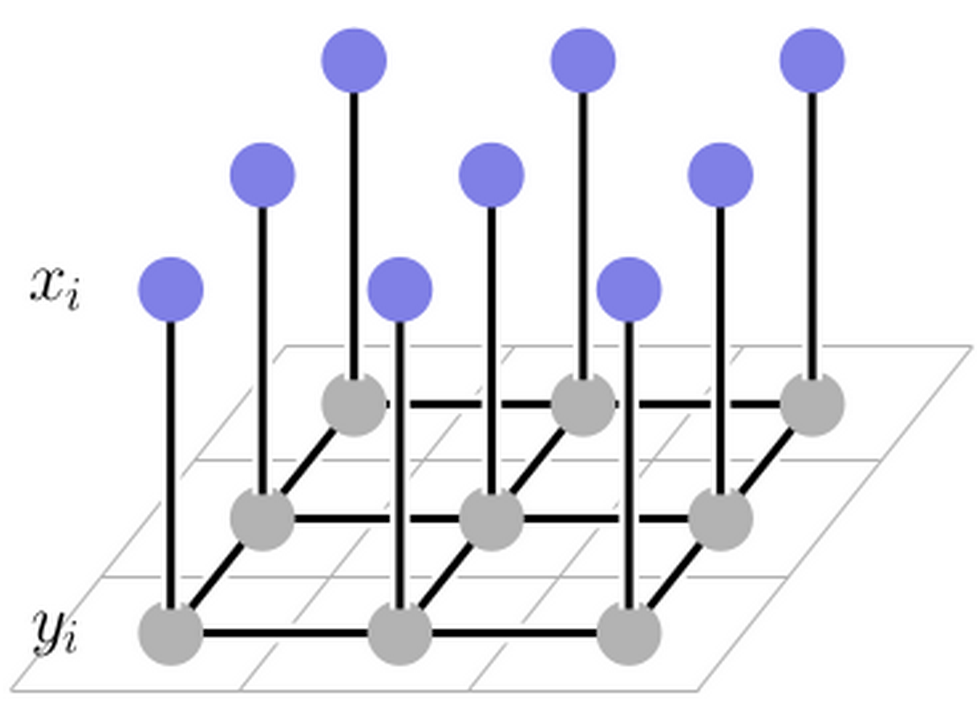
\includegraphics[width=0.7\textwidth,natwidth=610,natheight=642]{images/crfImage.png}
  \caption{Visualization of a Conditional random field for image segmentation where $y_i$ are the super-pixel labels, the edges between $y_i$ are the pairwise potentials, $x_i$ are the unary features of that super pixel and the edges between $x_i$ and $y_i$ are the unary potentials} 
  \label{fig:crfgraphic}
\end{figure} 

\par  More specifically the conditional random field has 1 node per super-pixel representing its label which has a unary potential linked to its unary-feature node and a pairwise potential linked to each of its neighbours. Considering each pixel a part of a joint output domain results in an output space of $K^n$, where $K$ is the number of possible labels and $n$ is the number of pixels or super-pixels. Due to this large domain standard classification methods will not work, in this paper we take the Structured Support Vector Machine (SSVM) approach. 
\section{The Pipeline}
For color or grayscale 3D tif stacks image data super-pixels are constructed with the Simple Linear Iterative Clustering (SLIC) algorithm. The super-pixel to pixel assignment mask is then used to construct a graph where each node receives a feature vector calculated from only the pixels assigned to this super-pixel. The ground truth is transformed into a graph with the same mask by assigning each node the label which the majority of its pixels have. This training dataset is then used to learn an SSVM with Block Coordinate Frank-Wolfe  (BCFW). The training occurs in equal partitions locally on different machines; at the end of every round the accumulated weights are recombined by the master node. Each the executor machines find the most constraining possible next update direction, this sub-problem is called the max-oracle. We implemented Mean Field to perform the max-oracle step but also included Loopy Belief propagation from the factorie package\cite{mccallum09:factorie:}.  The moving of data and managing computational resourches is done through the SPARK framework\cite{spark} with the CoCoA algorithm, which is designed to reduce lower network traffic. CoCoA and the BCFW solver is taken from the dissolve-struct framework \cite{dissolvestructWeb}. Once training is completed the model is again synchronized on the executor node and prediction is performed on the test dataset. 

\todo{Add image showing. Original Image, Super-pixel Boundaries,real ground truth, Ground truth interms of super pixels, a graph with labels and features, some image representaing and SVM, and then predicted outcome again interms of pixels} 

\section{Compare To other work}

For the super-pixel preprocessing step of our pipeline we choose to use SLIC super-pixels because of its time complexity and ability to control the number and shape regularity of the resulting super-pixels. Regularity of super-pixels in space is important to our model because it does not retain any information about the original spacial relations between pixels except for which super-pixels where neighbours during preprocessing. For the SSVM solver we chose BCFW because it can be distributed over $n$ machines if the dataset has $n$ training examples and has good convergence properties even with approximate max-oracle solvers \cite{lacoste2012block}.
\subsection{Super-pixel Alternatives}
One group of alternative super-pixel generation algorithms are graph based. Where in each pixel is initially considered to be a single node in a graph with undirected edges to its adjacent pixels. The edges are assigned weights based on a feature map including information from both neighbours member pixels. Then standard graph processing algorithms are used to minimize a global energy function over this graph resulting in a disconnected graph of super-pixels. 
One such algorithm is the Normalized cuts algorithm \cite{shi2000normalized}. The global criteria, defined by normalized cut, captures information of total dissimilarity between node grouping and also total similarity within the groups. The segmentation algorithms based on this criteria can achieve a computational complexity of $\mathcal{O}(N^{\frac{3}{2}})$ \cite{levinshtein2009turbopixels}. While the algorithm has had some success \cite{mori2005guiding} we prefer SLIC for 3D images due to its lower complexity of $\mathcal{O}(N)$. 
\par
Another graph approach was proposed by Fezenszwalb and Huttenlocher \cite{felzenszwalb2004efficient} which performs well with images that include both high variance and low variance regions. The algorithm performs global clustering where each super-pixel is the smallest spanning tree to cover its pixels. This approach has a better time complexity of $\mathcal{O}(N\log N)$ but in contrast to SLIC it does not have the ability to control the number of super pixels or the regularity of their shapes. 
\par 
A non parametric approach was introduced by Comaniciu and Meer which performs a recursive mean shift in the direction of the nearest stationary point of an underlying density function to find the mode of the distribution \cite{comaniciu2002mean}. It has been shown that this algorithm is equivalent to the Nadaray-Watson regression kernel. Again this algorithm does not have the ability to control the number or shape of the resulting super-pixels. 
\par
An empirically faster mode seeking algorithm, Quick Shift, was introduced in 2008 \cite{vedaldi2008quick}. The algorithm, for each pixel, finds the closest pixel in terms of increasing the Parzen density estimator and then moves them together. While it is quiet fast this algorithm also can not control the number or compactness of the resulting super-pixels. 

\subsection{SSVM Solver Alternatives}

The most common way of solving SVMs are the stochastic gradient descent algorithms (SGD). The direct generalization if SGD for problems with objective functions which are not differentiable, the stochastic sub-gradient descent algorithm (SSGD), has found some applications in structured learning \cite{ratliff2007approximate} \cite{tsochantaridis2005large} \cite{roller2004max}. Stochastic sub-gradient descent has a good convergence rate of $\tilde{O}(\frac{1}{\varepsilon})$ and like BCFW only requires on max-oracle call. But SSGD applies line search to an objective that is not differentiable may result in convergence to a suboptimal point. To avoid this problem and actually achieve the stated convergence rate it is assumed the user has specified an appropriate sequence of step sizes for the given problem \cite{ratliff2007approximate}. This additional tuning parameter of the step-size sequence is not required for BCFW because we can calculate the optimal step-size per iteration. 

\subsection{Alternative Software Packages}
NiftySeg is a 3D Image segmentation framework targeting brain imagery. It uses EM based segmentation with good performance on their data. Another valuable portion of the framework are the features specially designed for MRI images\cite{cardoso2011niftyseg}. NiftySeg is a very useful tool in its specific field of application but as it is not a distributed system the size of the datasets it can reasonably process are limited. 
\par
Another specialized open-source framework was published in 2013 named NIRFAST \cite{jermyn2013fast}. It is specialized for MRI images and utilizes blood oxygen saturation, water content and lipid concentration to construct the image segments. But again this framework was not designed to run on a distributed system. 
\chapter{Theory}


The notation we use here is a modified version of the notation used in \cite{lucchi2012structured} and \cite{lacoste2012block}. While we will reproduce the relevant information here \cite{lacoste2012block} is the original publication of the BCFW solver and \cite{slicPaper} is the original publication of the SLIC super pixel algorithm. 
\section{Recall Support Vector Machines}
The traditional binary Support Vector Machine problem can be stated as finding the best weight vector $w$ to correctly classify all multidimensional data points $x \in \mathcal{X}$ based on their features $\Phi(x)$
\begin{align}
y(x)=w^T\Phi(x)
\end{align} If $t_n \in\{-1,1\}$ is the n'th true label for $x_n$ we can formulate the maximum margin optimization problem as :
\begin{align}
\argmax_w\{ \frac{1}{||w||} min_n [t_n (w^T\Phi(x_n))] \}  
\end{align}
Considering that re-scaling $w$ does not effect the distance of any point to the decision plane we can scale  them such that $t_n(w^T\Phi(x_x))\geq 1$ holds for all points.  We can drop the $min_n$ term from the optimization objective by adding the $t_n(w^T\Phi(x_x))\geq 1 \forall x_x$ constraint because due to the $w$ rescaling there will always be at least one point for which the above statement is an equality. By this transformation we arrive at the canonical primal definition: 
  \begin{align}
  \argmin_w \frac{1}{2} ||w||^2 \quad S.T. \\ 
  t_n(w^T\Phi(x_x))\geq 1 
  \end{align} 
 
  \par When contrasting SVM methods with the basic Perceptron one can recognize that a Perceptron can find many different decision boundaries between the classes depending on what the ordering of that dataset was or what $w$ was initialized. The SVM has jointly optimizes the misclassification error and the margin of the support vectors. For a detailed comparison see \cite{meyer2003support}. It is intuitive to think that choosing the decision boundary which has the largest margin would minimize the generalization error, and it has indeed been shown theoretically that maximizing the margin minimizes bounds on the generalization error \cite{boser1992training}.
  
\par Alternatively to solving the primal formulation directly we can solve it in the dual. The dual formulation allows us to use kernel function; and later we will see for our large dimensional problem the dual parameters can be very sparse which provides computational advantages. To construct the Dual problem we differentiating the Lagrangian and substitute back into $L(w,a)$.
  \begin{align}
L(w,a) = \frac{1}{2}||w||^2 - \sum^{N}_{n=1} a_n { t_n ( w^T \Phi(x_n)) -1 }  \quad  S.T. \\
 w =\sum^{N}_{n=1} a_n t_n \Phi(x_n) \\ 
 0=\sum^{N}_{n=1} a_n t_n 
  \end{align}
  
  Which leads us to the canonical dual representation:
  
  \begin{align}
 \argmax_a \sum^N_{n=1} a_n -\frac{1}{2} \sum^{N}_{n=1} \sum^{N}_{m=1} a_n a_m t_n t_m \Phi(x_n)^T\Phi(x_m)  \quad  S.T. \label{eq:dualsvm}\\
 a_n \geq 0, \forall_n\\
 \sum^{N}_{n=1} a_n t_n =0
  \end{align}
  
\subsection{Duality Gap}
\par The dual solution is not necessarily exactly equivalent to the primal solution as the Lagrangian is only equal in the limit. The difference between the primal and dual is called the duality gap. It is possible for the gap to be zero, referred to as strong duality, but in most cases it is sufficient to compute the duality gap every couple of rounds to see if it is below a certain threshold in order to decide to stop iterating the solver. 
\subsection{SVM with High Class count}
When using an svm for a problem with more than 2 classes one must train several classifiers with one pivot class. If we have classes [A,B,C] then we train two SVMs [ $SVM_{A vs B}(x_n)$,  $SVM_{A vs C}(x_n)$ ] predict labels by choosing the label which got the best score vs A or we predict A if both SVMs labelled it as A. This method of classification is computationally inefficient especially for problems with large numbers of classes. Image segmentation is a problem with a massive class space because we do not simply have the $R$ number of labels which a pixel could take but we have the combination of labels over the entire image, hence the number of possible labels for a single image is $R^n$ where n is the number of pixels. 

\section{Structured Support Vector Machine } \label{ssvm}
Structured Prediction is the category of machine learning techniques designed to work with data that is more complex than a real valued outcome variable. The data will be expressed in a model which describes the relations between subsets of the data. In our image segmentation problem the output domain $y \in \ySpaceNoI(x)$ is the set of all possible label configurations for a given image x. And $x \in \xSpace$ is the set of all possible images. Structured Support Vector machines generalize the maximum margin approach to this kind of data. The standard approach for constructing a SSVM is to define a joint feature mapping $\Phi : \xSpace \times \ySpaceNoI \rightarrow \mathbb{R}^d $ which can include a measure of distance between two $y$ and also between different images $x$. On this joint feature space we again learn a linear function to the output, in contrast to the SVM, predicting requires maximizing over the possible labels $ \argmax_{y \in \ySpace} \lossFn(\yVec)-\langle \weightVec, \jointFeatureMap \rangle  $. With a training dataset $D = { (x_i,y_i)}^n_{i=1}$, we estimate $w$ by minimizing : 

 \begin{align}
 \min_{\weightVect,\error} \frac{\lambda}{2}||\weightVect||^2 + \frac{1}{2}\sum^n_{i=1}\error_i \label{optimizationFunc}  \quad  \text{S.T.}\\
\langle \weightVect,\jointFeatureMap \rangle \geq L(\yVect_i,\yVect) - \error_i \quad \forall i, \forall \yVect \in \ySpaceNoI(x_i) 
\end{align}

$ \textnormal{where} \quad \jointFeatureMap := \theta(x_i,y_i) - \theta(x_i,y) \textnormal{,} \quad L_i(y) := L(y_i,y) $ and $L(y_i,y)$ is the distance between the true label configuration and a possible other label configuration, typically we use the hamming distance here. The slack variable $\error_i$ holds the accepted error in this soft-margin formulation and $\lambda$ is the regularization parameter. 

This first formulation still has exponential number of constrains due to $\ySpaceNoI(x_i) $, but we can alleviate this issue by replacing the $\sum_{i} | \ySpace |$ linear constraints with $n$ piecewise-linear constraints as defined by this hinge-loss: 
\begin{align} \label{eq:maxOracle}
\shloss := \max_{y \in \ySpace} \lossFn(\yVect) - \langle \weightVec, \jointFeatureMap \rangle
\end{align}
\begin{align}
 \min_{\weightVect} \frac{\lambda}{2}||\weightVect||^2 + \frac{1}{n}\sum^n_{i=1} \shloss \label{optimizationFunc} \quad  \text{S.T.}\\
  \error_i \geq \shloss
\end{align}

The calculation of $\shloss$ is also referred to as the "max oracle", it is typically implemented with computational tricks to avoid a lot of the complexity of performing the $\max$ directly. In the following sections we assume an efficient solver for $\shloss$ exists. 

\subsection{Dual formulation SSVM}

There are $m:=\sum_i |\ySpace|$ variables which could become support vectors. In this formulation we use $\alpha_i(\yVect)$ as the dual variable associated with the training example $i$ and $\yVect \in \ySpace$ as the potential output. Solving the Lagrangian for the SSVM similar to \ref{eq:dualsvm} results in the following dual form:
\begin{align}\label{eq:ssvmDual}
\min_{\alpha \in \mathbb{R}, \alpha \geq 0 } f(\alpha) := \frac{\lambda}{2} ||\dualA \alpha||^2 - \dualb^T \alpha   \quad  \text{S.T.}
\end{align}
\begin{align}
\sum_{\yVect \in \ySpace} \alpha_i(\yVect) = 1 \quad \forall i \in [n]
\end{align}
where $\dualA \in  \mathbb{R}^{d \times m}$ is the column matrix $\dualA := \{ \frac{1}{\lambda n} \jointFeatureMap \in \mathbb{R}^{d} | i \in [n], \yVect \in \ySpace \}$ and  $\dualb := ( \frac{1}{n}\lossFn(\yVect))_{i \in [n], \yVect \in \ySpace}$. In this formulation we will have a very sparce representation in the dual variable vector $\alpha$ which is advantageous for sub-gradient optimization. With the Karush-Kuhn-Tucker conditions we can map between the dual and primal forms $\weightVec = \dualA \alpha = \sum_{i,\yVect \in \ySpace} \alpha_i(\yVect) \frac{\jointFeatureMap}{\lambda n}$. Computing the gradient of \ref{eq:ssvmDual} we find $\nabla f(\alpha) = \lambda \dualA^T \dualA \alpha - \dualb = \lambda \dualA^T \weightVec - \dualb$. Aditionally note that the domain of $f(\alpha)$ is the product of $n$ proabability simplicies, $\dualParamSpace := \Delta_{| \ySpaceNoI_1|} \times ... \times \Delta_{|\ySpaceNoI_n|}$.
It will show later that the sparsity in $\alpha$ and the ability to easily move back to the primal will be crucial for solving high dimensional problems. 

\section{Quadratic Programming Solvers}
\subsection{Frank-Wolfe optimization}
The Frank-Wolfe algorithm, originally published in 1956 \cite{frank1956algorithm}, is a quadratic programming solver with the same wide applications as typical sub-gradient methods as it only requires optimizing linear functions over the feasible set $\dualParamSpace$. It is applicable to any convex optimization problem where the feasible set $\dualParamSpace$ is compact and the objective $f$ is convex and continuously differentiable. The basics steps of the algorithm start with choosing a feasible search corner $\bm{s}$ by minimizing the linearisation of $f$ (using the current $\alpha$) constrained on being inside  $\dualParamSpace$. 
\begin{figure}[H]
  \centering
 \includegraphics[width=0.5\textwidth]{images/algo-3d-fw-alpha-figure.pdf}
  \caption{ } 
  \label{fig:frankwolfe}
\end{figure} 
All following steps are a convex combination of a new $\bm{s}$ and the previous iteration with some step-size $\gamma$.  This formulation is advantageous for problems when $\alpha$ is in high dimensions, as the current $\alpha$ can be expressed in terms of the the initial $\alpha^{(0)}$ and all  $\bm{s}$ corners selected in the iterations leading up to the current round. An $\alpha$ that can be written in this form can be stored in memory as a sparse object and hence never needs to allocate memory, without this property an $\alpha$ for image segmentation would never fit into memory. Additionally Frank-Wolfe has the advantage that we can compute the duality gap for free, because $f$ is convex its minimization over $\dualParamSpace$ is a lower bound on the value of the globally optimal $f(\dualAlpha^*)$. Being able to compute the duality gap allows us to monitor the progress of the algorithm over time and also allows us to choose a theoretically sounds stopping criteria $f(\dualAlpha) - f(\dualAlpha^*) \leq \epsilon$. It has also been shown \cite{dunn1978conditional} that the algorithm converges to a $\epsilon$-approximate solution within $\mathcal{O}(\frac{1}{\epsilon})$

\begin{samepage}
  \rule{\textwidth}{2pt}
\begin{algorithm}[H]\label{algo:bcfw}
     Let $\alpha^{(0)} \in \dualParamSpace$\;
     \For{$k = 0 $ ... $ K$}{
    	Compute $\bm{s} := \argmin_{\bm{s}^\prime \in \dualParamSpace} \langle \bm{s}^\prime,\nabla f(\bm{\alpha^{(k)}} \rangle$ \;
        Let $\gamma := \frac{2}{k + 2}$ or optimize $\gamma$ by line-search
        update $\bm{\alpha}^{(k+1)} := (1 - \gamma) \bm{\alpha}^{(k)} + \gamma \bm{s}$
     }
     \caption{ Frank-Wolfe on a Compact Domain  }
  \end{algorithm}
\hrulefill
\end{samepage}

\subsection{Block Coordinate Frank-Wolfe} \label{bcfw}

A disadvantage of the Frank-Wolfe algorithm described above is that it requires $n$ calls to the maximization oracle for SSVMs. The Block-Coordinate Frank-Wolfe algorithm \cite{lacoste2012block} improves this to only requiring one call to the maximization oracle in the context of SSVMs. The method described \cite{lacoste2012block} and reproduced here in Algorithm \ref{algo:bcfw} can be applied to any constraint optimization problem of the form 
\begin{align}
\min_{\alpha \in \dualParamSpace^1 \times ... \times \dualParamSpace^n} f(\alpha)
\end{align}
having a Cartesian product over $n \geq 1$ blocks as the domain $\dualParamSpace = \dualParamSpace^1 \times ... \times \dualParamSpace^n \subseteq \mathbb{R}^m $. The reduction in oracle calls comes from this structure in $\dualParamSpace$. This structure allows  to perform cheap update steps affecting only one variable block $\dualParamSpace^{(i)}$ instead of optimizing the entire problem simultaneously. We assume that each factor is convex and compact $\dualParamSpace^{(i)} \subseteq \mathbb{R}^{m_i} $, with $m = \sum^n_{i=1} m_i$. In the following $\dualAlpha_i \in \mathbb{R}^{m_i}$ for the $i$-th block of coordinates of a vector $\dualAlpha \in \mathbb{R}^m$. The iterative root of Algorithm \ref{algo:bcfw} chooses one block uniformly at random and leaves the other blocks unchanged. If we only had one partitioning i.e. $n=1$ then Algorithm \ref{algo:bcfw} is equivalent to the original Frank-Wolfe algorithm. 

\begin{samepage}
  \rule{\textwidth}{2pt}
  \begin{algorithm}[H]\label{algo:bcfw}
     Let $\alpha^{(0)} \in \dualParamSpace^{(1)} \times ... \times \dualParamSpace^{(n)}  $\;
     \For{$k = 0 $ ... $ K$}{
      Pick $i$ at random in \{1, ... ,n \}\;
      Find $\bm{s}_{(i)} := \argmin_{\bm{s}_{(i)}^\prime\in \dualParamSpace} \langle \bm{s}_{(i)} ^\prime\nabla_{(i)}f(\bm{\alpha}^{(k)} \rangle$ \;
      Let $\gamma := \frac{2 n}{k + 2n}$ or optimize $\gamma$ by line-search\;
      Update $\bm{\alpha}_{(i)}^{k+1} := \bm{\alpha}^{(k)}_{(i)} + \gamma (\bm{s}_{(i)} - \alphaVec_{(i)}^{(k)} )$\;
     }
     \caption{ Block-Coordinate Frank-Wolfe Algorithm on product Domain }
  \end{algorithm}
  \hrulefill
\end{samepage}

Another advantage of BCFW over other methods like Stochastic Gradient Descent is that we can compute our optimal step-size $\gamma$ in closed form. 

\subsubsection{BCFW for the SSVM}
For our image segmentation applications we used the BCFW algorithm \ref{algo:bcfw_ssvm} for SSVMs such that we only need to maintain the primal $w$. The equivalence between Algorithm \ref{algo:bcfw} and Algorithm \ref{algo:bcfw_ssvm} rests on the  relations : $\wv_s = \dualA\bm{s}_{[i]}$ and $\ell_s = \dualb^T\bm{s}_{[i]}$ in the primal update. Where $\bm{s}_{[i]}$ is a zero-padded version of $\bm{s}_{(i)} := \bm{e}^{\yVect_i^*} \in \dualParamSpace$ such that $\bm{s}_{[i]} \in \dualParamSpace$. 

\begin{samepage}
  \rule{\textwidth}{2pt}
  \begin{algorithm}[H]\label{algo:bcfw_ssvm}
   Let $\weightVec^{(0)}:=\weightVec^{(0)}_i := \bar{\weightVec}^{(0)} := 0$,\quad $\ell^{(0)} := \ell_i^{(0)} := 0$\;
   Using $\oracleobj_i(\yVec,\weightVec^{(k)}) := \oracleexp$ \;

   \For{$k = 0$ ... $K$}{
     Pick $i$ at random in \{1, ... ,n \}\;
     Solve $ \yVec^*_i := \argmax_{\yVec \in \ySpace} \oracleobj_i(\yVec,\weightVec^{(k)})$ \;
     Let $\weightVec_s := \frac{1}{\lambda n} \jointFeatureMapAlone_i(\yVec^*_i)$ and $\ell_s := \frac{1}{n}\lossFn(\yVec_i^*)$\;
     Let $\gamma := \frac{\lambda (\wv_i^{(k)} -\wv_s)T \wv^{(k)} - \ell_i^{(k)} + \ell_s}{\lambda ||\wv_i^{(k)} - \wv_s||^2}$ and clip to $[0,1]$\;
     Update $\wv_i^{(k+1)} := (1 - \gamma)\wv_i^{(k)} + \gamma \wv_s$ and $\ell_i^{(k+1)} := (1 - \gamma) \ell_i^{(k)} + \gamma \ell_s$ \;
     Update $\wv^{(K+1)} := \wv^{(k)} + \wv_i^{(k + 1)} - \wv_i^{(k)}$ and $\ell^{(k+1)} := \ell(k) + \ell_i^{(k+1)} -\ell_i^{(k)}$ \;
     (Optionally: Update $\bar{\wv}^{(k + 1)} := \frac{k}{k+2}\bar{\wv}^{(k)}+\frac{2}{k+2}\wv^{(k+1)}$ )

   }
   \caption{ Block-Coordinate Frank-Wolfe Algorithm for SSVM}
  \end{algorithm}
  \hrulefill
\end{samepage}


where $\oracleobj_i(\yVec,\weightVec^{(k)}) := \oracleexp$ is the hing loss as used in  \ref{eq:maxOracle}. 

Important for our Image segmentation application is that these BCFW convergence properties also hold if the max oracle is solved approximately. We simply require that the oracle gives a candidate direction $s_{(i)}$ with multiplicative accuracy $\nu \in (0,1]$ in terms of the duality gap on the current block \cite{lacoste2012block}. But with approximate oracles there is a slow down in convergence inversely proportional to the accuracy at $\frac{1}{\nu^2}$. We will utilize this property in order to quickly find an approximate maximal energy with variational methods. 

\section{CRF Models}
The following model describes the basis of how we construct the joint feature function $\jointFeatureMapAlone$ used in the SSVM formulation \ref{eq:maxOracle}. The SSVM is expressed as a quadratic programming problem hence the constraints must be linear. We express the energy function $E_w$ as an inner product of the features and the weight vector $w$. Our CRF energy is separated into its unary and pairwise portion. 
\begin{align}
D_i(y_i) = \langle \weightVec^D, \crfFeatMap^D_i(y_i) \rangle \\
V_{ij}(y_i,y_j) = \langle \weightVec^V, \crfFeatMap^V_{i j}(y_i,y_j) \rangle
\end{align}
where $\crfFeatMap^D(y_i)$ and $\crfFeatMap^V_{i j}(y_i,y_j)$ are feature maps dependent on both the observed data and the labels. 
\begin{align}
\crfFeatMap^D(y_i) = (I(y_i= 1 )x_i^T, ..., I(y_i = K)x_i^T)^T, 
\end{align}
where $x_i$ is the feature vector associated with super pixel node $i$,  $K$ is the max label and $y_i \in \{ 1,...,K \}$. If $\weightVec^D$ is the column vector $[\weightVec^D_1,...,\weightVec^D_K]^T$ then the unary term of $E_w$ can be written as an inner product 
\begin{align}
D_i(y_i) = \langle \weightVec^D_{y_i},x_i\rangle,
\end{align}
Which gives the unary factor of node $i$ if it were labelled with $y_i$. The pairwise feature mapping can be defined similarly 
\begin{align}
  \crfFeatMap_{i j}^D(y_i,y_j) = (I(y_i = a, y_j = b))_{(a,b) \in \{ 1,...,K\}^2}
  \end{align}
    with parameters $\weightVec^V = (\weightsmall_{a b})_{(a,b) \in \{ 1,..., K\}^2 }$, then we can write the pairwise term as a simple indexing 
  \begin{align}
V_{i j} (y_i, y_j) = \weightsmall_{y_i y_j}
\end{align}
  This pairwise term defines the edge energy between adjacent node $i$ and $j$ as the learned cost in $\weightsmall$ of the transition between label $y_i$ and $y_j$. We now combine the unary and pairwise term by letting, $\weightVec = ((\weightVec^D)^T, (\weightVec^V)^T)^T$, $\crfFeatMapBig^D(Y) = \sum_{i \in \setOfVertecies} \crfFeatMap^D_i(y_i)$, $\crfFeatMapBig^V(Y) = \sum_{(i,j) \in \setOfEdges} \crfFeatMap^V_{i j} (y_i, y_j)$ and  $\crfFeatMapBig(Y) = [ \crfFeatMapBig^D(Y)^T, \crfFeatMapBig^V(Y)^T ]^T$ to define the total energy of a CRF as an inner product 
\begin{align}\label{eq:crfenergy}
E_{\weightVec} (Y) = \langle \weightVec, \crfFeatMapBig(Y) \rangle 
\end{align}
  where $\setOfVertecies$ is the set of vertices of super-pixels extracted from the input image and  $\setOfEdges$ is the set of edges. For a visualization see Figure \ref{fig:crfgraphic}. 
\subsection{CRF model variations}\label{sec:crfvariations}
Of the three CRF models we used to describe our image segmentation data, the unary model is the simplest and also the only one where we can in a reasonable amount of time compute an exact solution to the max-oracle problem. 
\subsubsection{Unary CRF Model}\label{sec:unaryModel}
In what we call the unary model each super pixel label node is simply connected to its unary potential which simplifies the energy function too
\begin{align} \label{mdl:unary}
E_{\weightVec^D} (Y) = \langle \weightVec^D , \crfFeatMapBig^D(Y) \rangle
\end{align}
\subsubsection{Pairwise CRF Model}\label{sec:pariwiseSimple}
The pairwise model contains the same factors represented in the unary model but also includes the edge potentials as described in \ref{eq:crfenergy}
\begin{align}
E_{\weightVec} (Y) = \langle \weightVec, \crfFeatMapBig(Y) \rangle 
\end{align}
\subsubsection{Data-dependent Pairwise CRF Model}\label{sec:dataDep}
The data-dependent pairwise model is an expansion of the pairwise model by redefining the pairwise energy as in 
\begin{align}
 \crfFeatMapBig^V(Y) = \sum_{(i,j) \in \setOfEdges} \crfFeatMap^{DV}_{i j}(y_i,yj)  \label{sec:dataDep}
 \end{align}
\begin{align}
  \crfFeatMap^{DV}_{i j}(y_i,y_j) = (I(y_i = a, y_j = b) * \dataDepFn^I_{i j} )_{(a,b) \in \{ 1,...,K\}^2}   %could work on this definition its not quiet clear 
\end{align} 
\begin{align}
\dataDepFn^I_{i j} =  (I(\dataDepFn(x_i,x_j)=c))_{c \in range(\dataDepFn)}
\end{align}
The function $\dataDepFn(x_i,x_j)$ is a binning function, with a small discrete range in $\mathbb{Z}$, it is used to give the pairwise term more flexibility to learn transition probabilities between labels under certain contexts. For examples of such functions and an analysis of the advantages of using a data dependent pairwise term see \cite{dataDepPaper1} and \cite{dataDepPaper2}.
\begin{description}
\item[Average Intensity Difference] For all neighbouring nodes $A$ and $B$ we calculate the average intensity (for RGB its also the grey-scale intensity) and simply take their squared difference. Quantiles are computed for the entire dataset and used to calculate fixed boundaries for binning the pairwise edges based on argument \inputArgs{numDataDepGraidBins}. 
\item[ Average Intensity Difference scaled by one hop neighbourhood Standard Deviation ] For all neighbouring nodes $A$ and $B$ we calculate the difference in average intensity divided by the sum of variances of the one hope neighbourhoods of both nodes (for RGB its also the grey-scale intensity). The values are calculated for all neighbours in the training set and sorted to find quantile boundaries which result in equal mass being binned to each group. The number of bins depends on argument \inputArgs{numDataDepGraidBins}. 
\item[ Average Intensity Difference scaled by two hop neighbourhood Standard Deviation ] For all neighbouring nodes $A$ and $B$ we calculate the difference in average intensity divided by the sum of variances of the two hope neighbourhoods of both nodes (for RGB its also the grey-scale intensity). The values are calculated for all neighbours in the training set and sorted to find quantile boundaries which result in equal mass being binned to each group. The number of bins depends on argument \inputArgs{numDataDepGraidBins}. 
\item[ Uniqueness difference ] For all neighbouring nodes we calculate the uniqueness in its one hop neighbourhood by the number of neighbourhood standard deviations away from the neighbourhood mean the super-pixel average intensity is. For any two neighbouring nodes $A$ and $B$ we then compute the difference in this uniqueness measure. The values are calculated for all neighbours in the training set and sorted to find quantile boundaries which result in equal mass being binned to each group. The number of bins depends on argument \inputArgs{numDataDepGraidBins}. 
\item[ Uniqueness in Opposite Neighbourhood ]  The internal super-pixel mean intensity $AvgI()$ and the average mean in its one hope neighbourhood $AvgNeigh()$ is calculated for all nodes. For every neighbouring nodes $A$ and $B$ we compute $(AvgI(A) - AvgNeigh(B))^2 + (AvgI(B) - AvgNeigh(A))^2$ as the total uniqueness of each node in the others neighbourhood. The values are calculated for all neighbours in the training set and sorted to find quantile boundaries which result in equal mass being binned to each group. The number of bins depends on argument \inputArgs{numDataDepGraidBins}. 

\end{description}

\section{Max Oracles}
 The problem defined by  $ \argmax_{\yVec \in \ySpace} \oracleexp $, depending on the structure of $\yVect$, it can be intractable. When modelling the image segmentation problem with a pairwise CRF as in \ref{sec:dataDep} then a naive maximization by calculating the energy for all $\yVec \in \ySpace$ would be intractable because $|\ySpace| = R^{|\yVec|}$ where $R$ is the number of possible labels and $|\yVec|$ is equal the number of super-pixels. Hence we must intelligently approximate this max-oracle or use a simpler model. 
\subsection{Naive Unary Max}\label{sec:unaryMax}
When solving a model with unary potentials only, as in \ref{mdl:unary}, we can find an exact solution with $\mathcal{O}(K|\yVect)i|)$ by simply evaluating the loss-augmented potential for each super-pixel node and every possible label. This method can actually get rather good results if the unary term include features which have information about the surrounding space or the classes have repeating patterns in each super pixel significantly distinct from the other classes. 

\subsubsection{Mean Field }\label{sec:meanField}
All variational methods approximate a difficult to compute true distribution $P$ with a distribution with lower computational complexity $Q$ which is close to the true distribution, in terms of the Kullback–Leibler divergence. The distance between $P$ and $Q$ is defined as $D_{KL}(Q||P) = \sum_{\bm{Z}} Q(\bm{Z}) \log \frac{Q(\bm{Z})}{P(\bm{Z}|\bm{X})}$, where $\bm{Z} $ are some unobserved variables and $\bm{X}$ is a dataset. In the case of our image segmentation problem $\bm{Z}$ are the hidden labels $\yVec$ and the data is $\xSpace$.
One of these variational methods is the Mean Field inference where in a computationally feasible $Q$ is constructed as a product of individual distributions for a subset of the unobserved variables i.e. $Q(\bm{Z}) = \prod_{i=1}^M q_i(\bm{Z}_i|X)$. In our image segmentation problem we could model the pairwise CRF as a series of Exponential distributions. The parameters of $Q$ can be quickly learned from the data with variational calculus. When considering the CRF visualization of Figure \ref{fig:crfgraphic}, mean field would prune all edges between the labels, but then find the distributions of the individual $q_i$ iteratively as a function of all other $q_i$.
\subsection{Loopy Belief Propagation}\label{sec:loopybp}
The Sum-Product algorithm is a message passing algorithm used to find marginals on Bayesian networks which can be expressed as trees \cite{sumProductAlgo}. We can transform a Bayesian network if it is a tree into a bipartite factor graph where each variable is a class variable in the Bayesian network and each factor is some probabilistic relation between variables (and hence has an edge to all those variables). If label a bipartite factor graph with factors $f_A, f_B, f_C ... = F$ and variables $x_1, x_2, x_3, x_4 ... = X $. Then we can quickly see that the marginal probability of a leaf is independent of the remaining graph variables given all factors it is connected too. The Sum-Product Algorithm then computes the marginal probabilities by applying the following rules to each node in the factor graph starting with the root. 
\begin{description}
\item[Product Rule]: At each variable node take the product of all its descendant
\item[Sum-product Rule] : At each factor node $i$ take the product of $f_i$ all its descendants and then sum over all variables except for the uncompleted parent node.
\end{description}
More precisely we can define the messages: 
\begin{align}
\shortintertext{Variable to factor message: } 
\mu_{x \rightarrow f}(f_i) = \prod_{h \in n(x)  \backslash f_i } \mu_{h \rightarrow x} \\
\shortintertext{factor to variable message: } 
\quad \mu_{f \rightarrow x}(x_i) = \sum_{x_j \in X \backslash x_i } ( f(x_j) \prod_{ y \in n(f) \backslash x_i } \mu_{y \rightarrow f(y)})
\end{align}
Where $\mu$ are types of messages, \textbackslash\{$a$\} define the set operator of excluding $a$, $n(a)$ is the set of neighbours of $a$. 
Using the Sum-Product algorithm one can compute all marginals in $\mathcal{O}(n^2)$ and with some additional rules recomputing factors can be avoided. 
\par
Loopy Belief Propagation is a extension on the Sum-Product algorithm which simply applies the same rules to a loopy graph in each iteration ignoring that it is actually not a tree. But in practice it has shown good results \cite{murphy1999loopy}. We expect good results on our super-pixel graph because the direct connections are by far the most important and do not depend on much more than their adjacent nodes. 
%
%
%
%
%
%
%
%
%
%
%
%
%


%
\chapter{SuperPixel Preprocessing}

The computationally most expensive step during the preprocessing stage of our pipeline is the construction of super-pixels. Once the super-pixels are constructed consider it one datapoint with its features and with one label. If we were to use a simple grid of square super-pixels we will have a large chance of summarizing features on a super-pixel which includes significant portions of two or more labels but the resulting training set will attribute the features coming form this area to just the label which had the highest pixel count even if that is only 51\% of the super-pixel. One way to minimize these overlapping features is to make the super-pixels small as the number of super-pixels which are on the edge between two objects is smaller than the area inside each object this will make the dataset cleaner overall. But the smaller we choose a super pixel the larger the resulting graph gets and for pairwise models the graph size has an exponential effect on the number of possible decodings for the max-oracle. Additionally if the super pixels are too small the unary features extracted from the may not be able to capture the signature patterns present in each object. We would like to choose a super-pixel size which optimizes these two criteria. With a fixed $S$ we are left with the specific boundaries of the super-pixel to combat the problem of overlapping features.

There are many super-pixel generation algorithms which attempt to align with edges of objects, since we are dealing with large images we choose to use the SLIC algorithm \cite{slicPaper}. 

\par
The SLIC approach is to perform a kind of localized k-means cluster on a unified space including the pixel value and its spacial coordinates. For RGB color images this space could be the the 6D space of [r,g,b,x,y,z]. If we where to run simple k-means on this space with a euclidean distance function we would run into problems do to the RGB space being bounded while the xyz space is not. Normalizing the spacial distance proportional to the selected super pixel size is one key difference to K-mean. In terms of complexity the key difference to K-means cluster is the assumption which allows SLIC to have a $\mathcal{O}(N)$ is that assignments to a super-pixel cluster will never be farther than $2S \times 2S \times 2S$ away from the center.  Resulting in $K(8S^3)$ or $8N$ assignments, since $S= \sqrt[3]{\frac{N}{K})}$, $K= \frac{N}{S^3}$. While the complexity of K-means is $\mathcal{O}(NK)$, SLIC has $\mathcal{O}(N)$. 


\section{SLIC Algorithm}\label{sec:slicAlgo}

Our ScalaSLIC implementation allows for general object datatype to be saved in each pixel location. If the user would like to cluster something other than RGB or grayscale images they must define distance functions on their datatype. For grayscale $d_{data}=\sqrt[]{(I_k-I_i)^2}$ where $I_k$ is the grayscale intensity of the cluster center and $I_i$ that of the to be compared pixel. For RGB $d_{data}=\sqrt{(l_k - l_i)^2+(a_k - a_i)^2+(b_k - b_i)^2}$ where [$l$,$a$,$b$] are the dimensions of the CIELAB color space. 
\\
\begin{samepage}
  \rule{\textwidth}{2pt}
\begin{algorithm}[H]\label{algo:slic}
Initialize cluster centers $C_k=[DataType_k,x_k,y_k,z_k]^T$ by sampling pixels at regular grid steps $S$.
Perturb cluster centers in a $3 x 3$ neighbourhood, to the lowest gradient position. 
     \While{ E $\leq$ threshold}{
       \For{each cluster center $C_k$}{
          Assign the best matching pixels from a $2S \times 2S \times 2S$ cube neighbourhood around the cluster center according to the distance measure $D_s = d_{data} + \frac{m}{S}\sqrt[2]{(x_k -x_i)^2 + (y_k - y_i)^2 + (z_k - z_i)^2}$
       }
       Compute new cluster centers 
       Compute residual error $E$ {L1 distance between previous centers and recomputed centers}
     }
     Enforce Connectivity
     \caption{ SLIC Super-pixels }
  \end{algorithm}
\hrulefill
\end{samepage}

\section{Super Pixel Size effect on Training time}
One of the key factors in dealing with our high dimensional data is to not consider each pixel individually but rather to create super-pixels which then make each image significantly lower dimensional. 
The difficulty of the problem depends on the number of possible $\yVect \in \ySpace$, by decreasing the size of the super-pixels the number of super pixels goes up with $
\yVect = (\frac{L}{S})^3$, where $C$ is the length of one edge of a cube volumetric image. The work required for the naive max-oracle on the unary model is $K(\frac{L}{S})^3$, where $K$ is the number of possible labels. For the pairwise CRF the naive approach of computing the energy for all possible $\yVect$ would be $K^{(\frac{L}{S})^3}$. Although LoopyBP does not try all possible $\yVect$ we expect the size of the graph to increase computation time more than for any unary based max-oracle. See Figure \ref{fig:superPixelSpeedup} for empirical results on total training time for both LoopyBP on a pairwise model and the Naive method on a unary model.
%
\begin{figure}
  \centering
  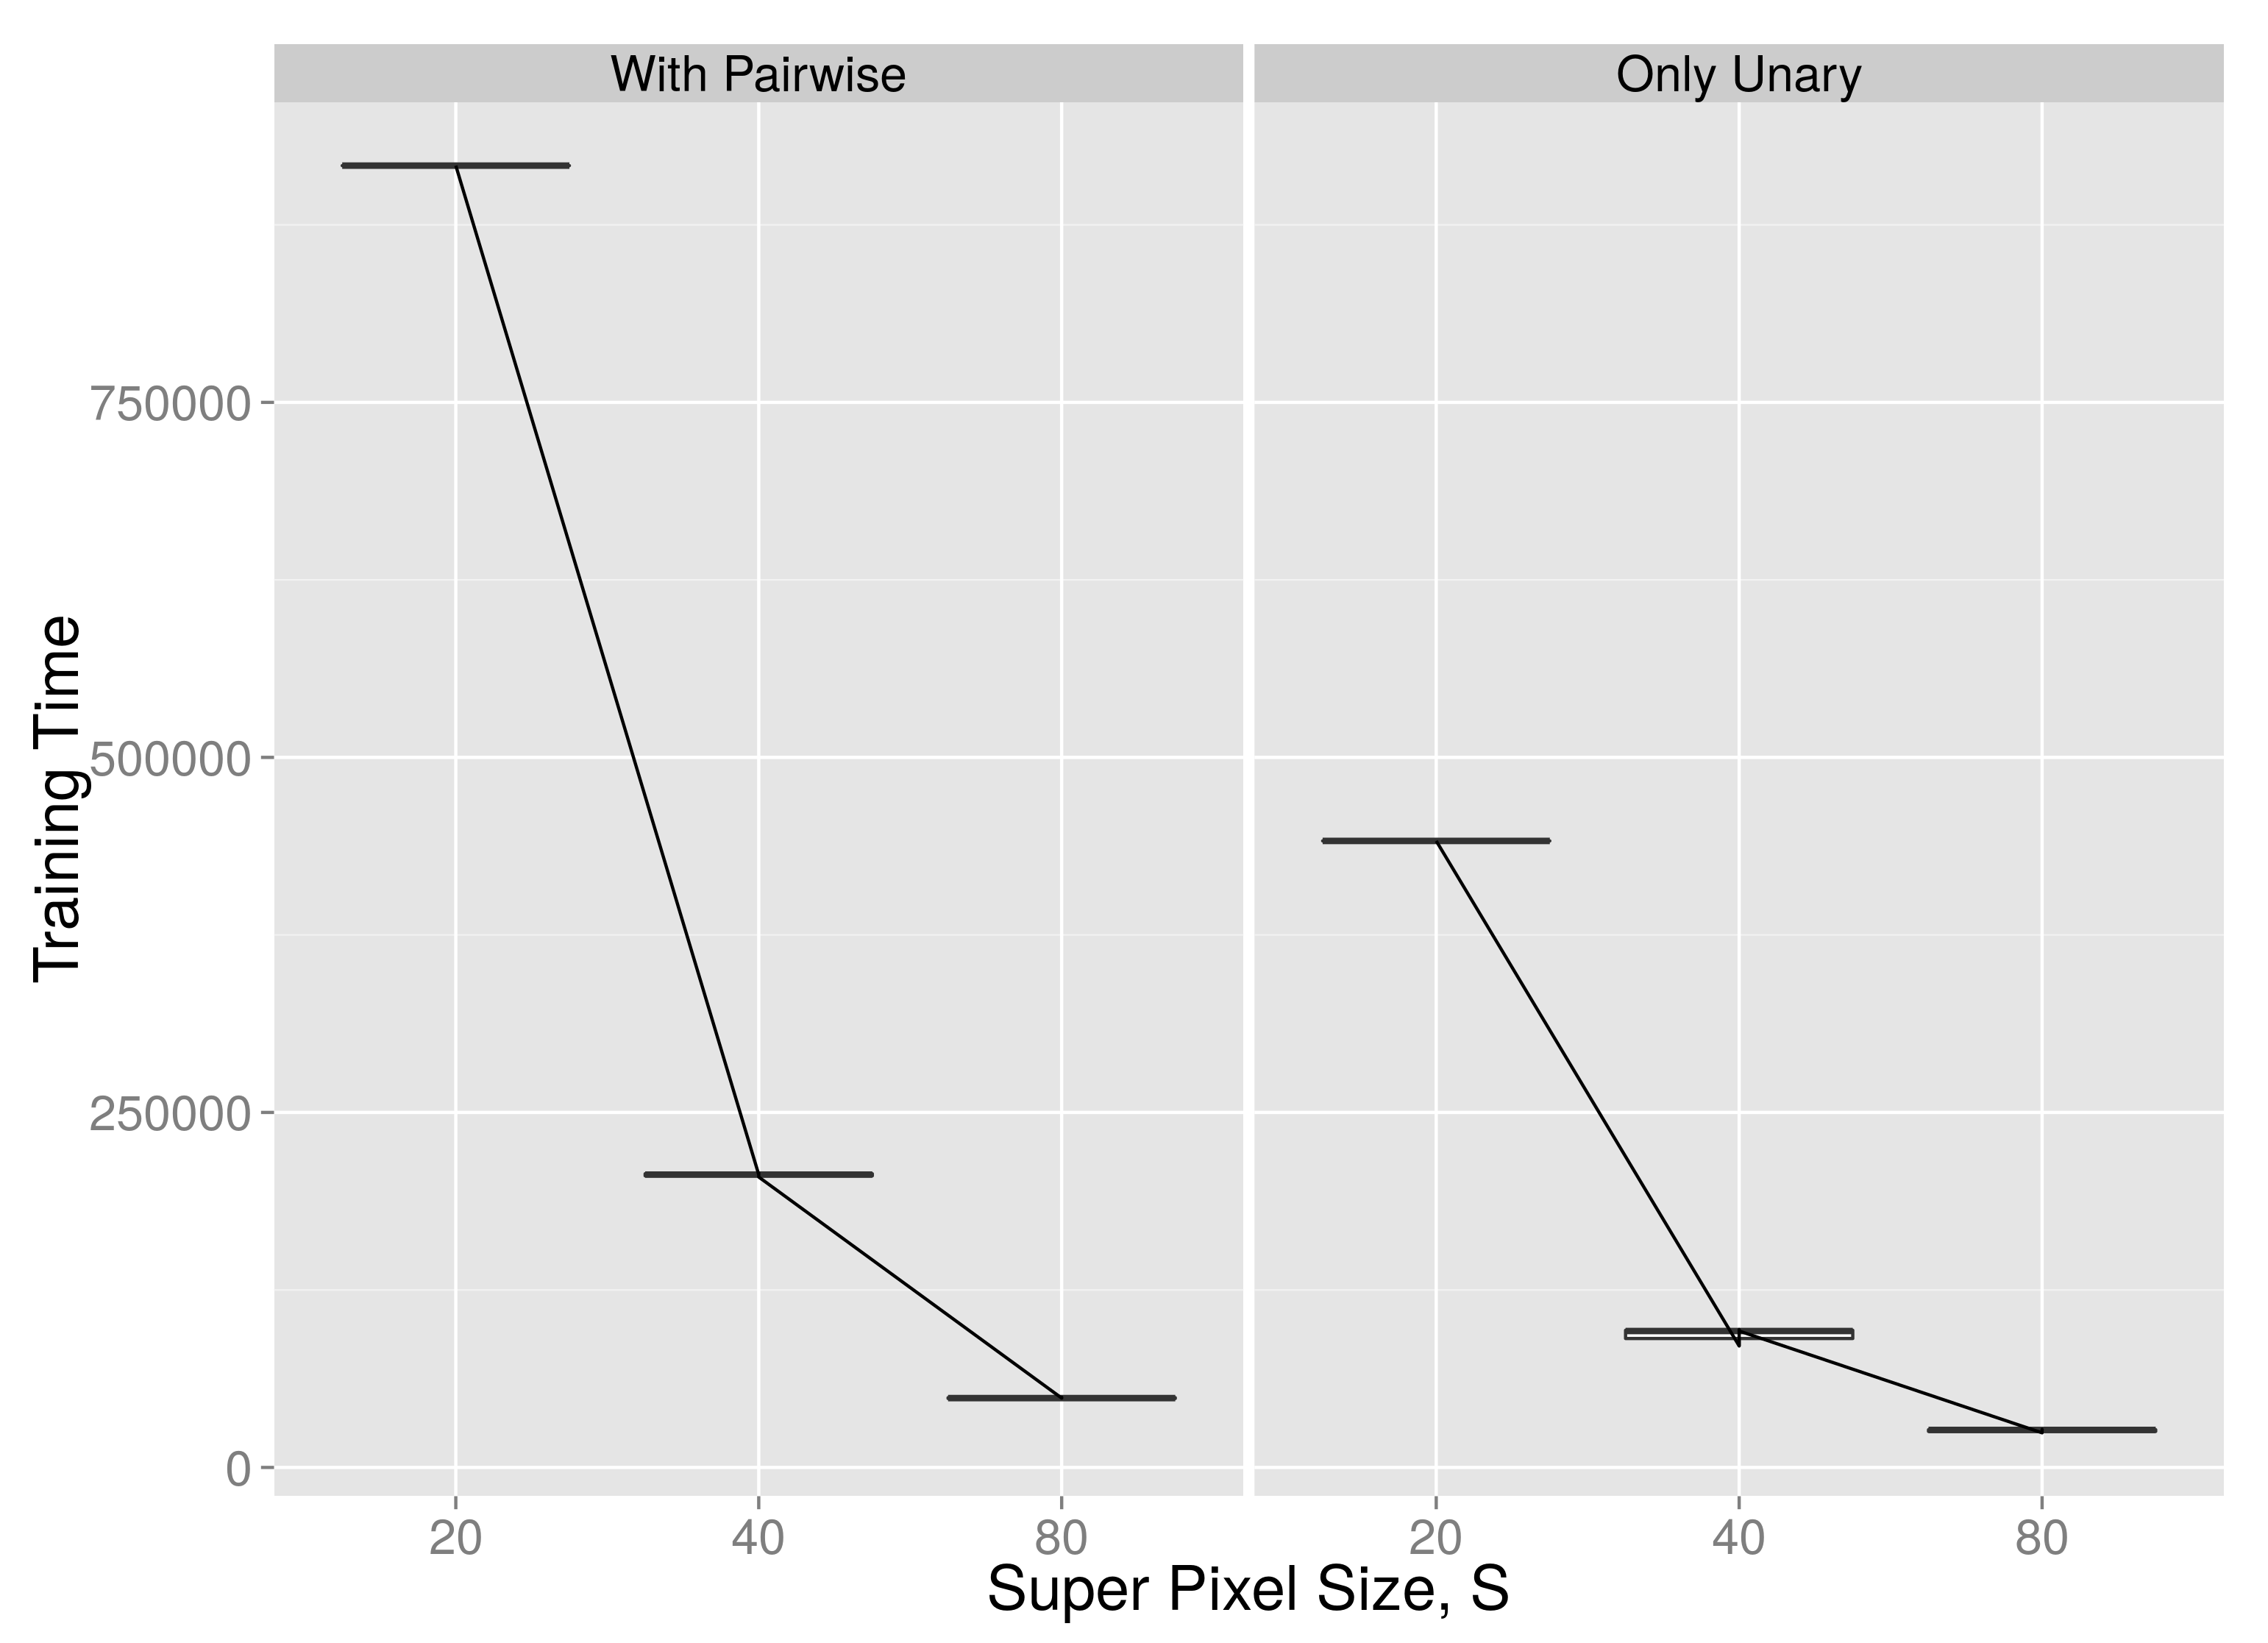
\includegraphics[width=0.8\textwidth]{images/SuperPixel_Speed_up.png}
  \caption{ Here we plot the total training time varying the size of super-pixels (and there fore the number of nodes in the graph). Larger graphs result in larger data volumes moving across the network but the primary time consuming function in our BCFW is the max-oracle. We repeat the same super-pixel resizing experiment with LoopyBP max-oracle and the Naive max for a unary model.} 
  \label{fig:superPixelSpeedup}
\end{figure} 
%



\section{SLIC vs Naive Squares}
When directly comparing the test scores of an SSVM trained on SLIC versus Square super-pixels we found that SLIC does in fact increase performance in both Unary and Pairwise models. 
In contrast to most figures here we are looking at the per pixel loss(see Figure \ref{fig:slicvssquarePix}. The UCSB Nuclei data set is largely skewed towards one class and hence we train on a loss that is weighted by the inverse class frequency. With loss weighting we also find a significant improvement in test loss on this Nuclei dataset, see Figure \ref{fig:slicvssquareNucli}.  


%
\begin{figure}
  \centering
  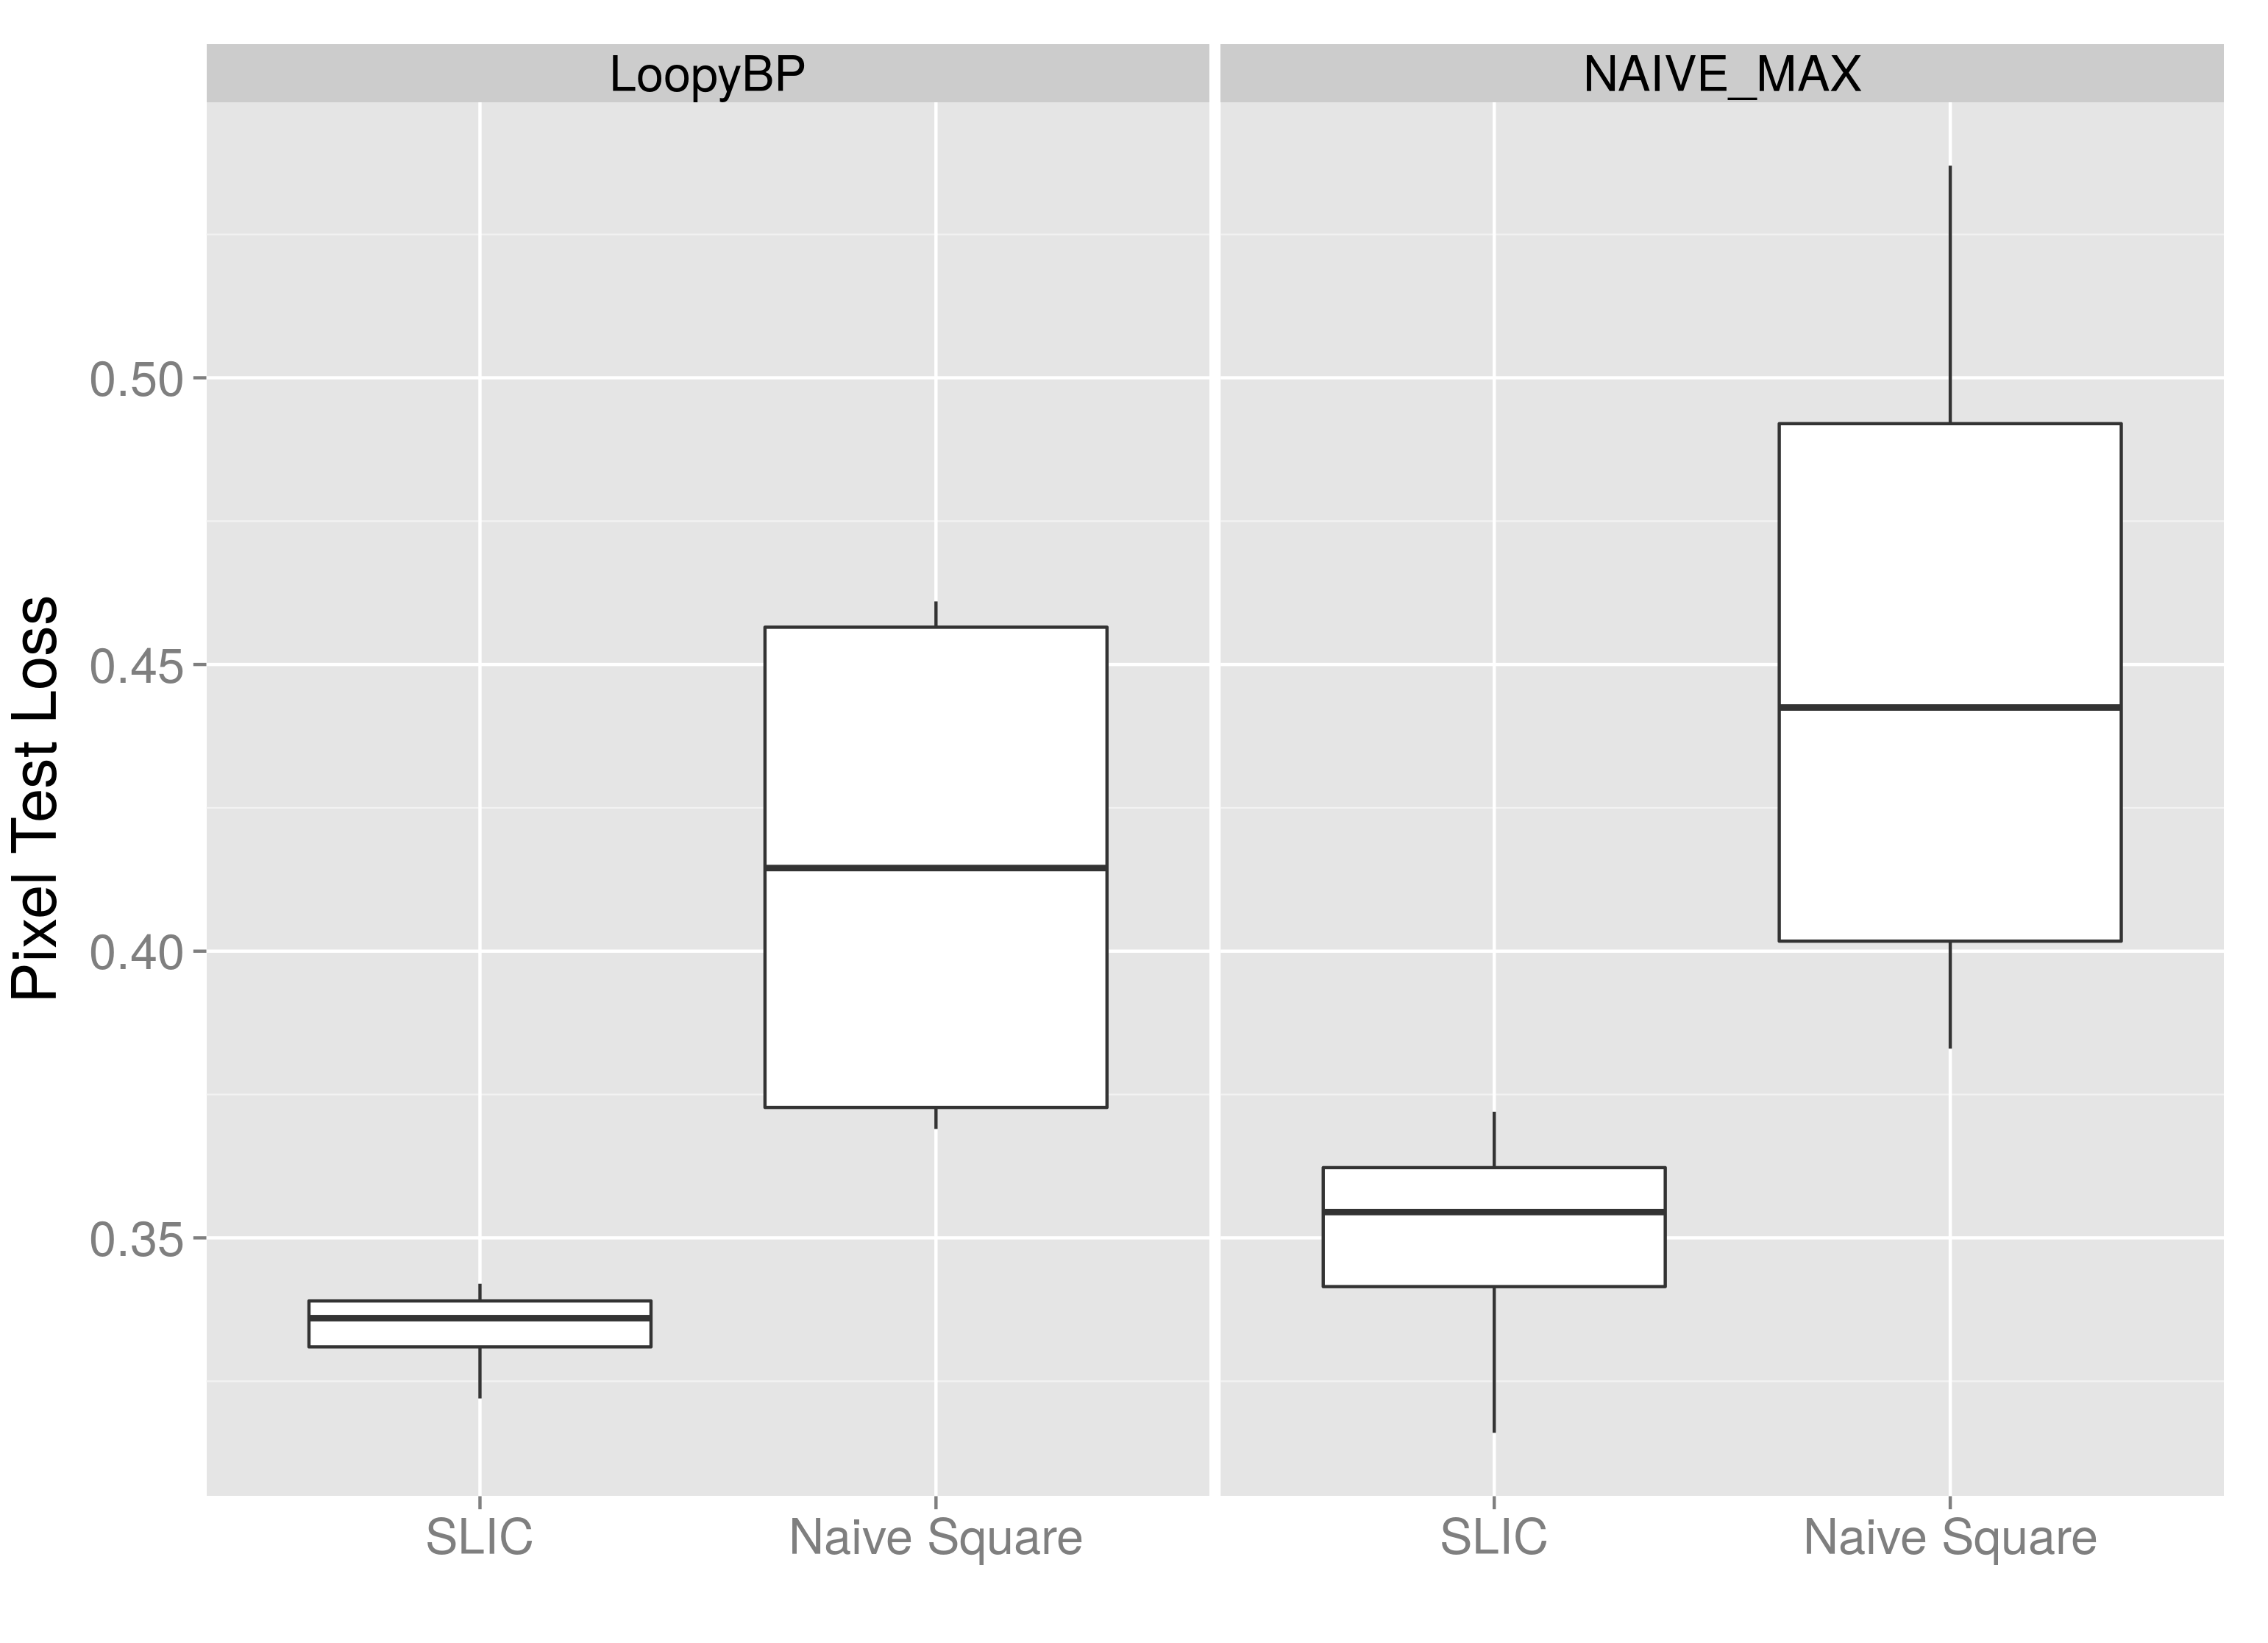
\includegraphics[width=0.8\textwidth]{images/slicVsNaiveSquare_pix_synGen.png}
  \caption{ Comparing the per pixel test loss using either SLIC or Square super-pixels. The experiment was repeated for Unary model and a Pairwise model solved with Loopy Belief Propagation.  Data ( SynthData see \ref{sec:synthDataGen}, WhiteNoise:0.40 SquarImgSize:30 OsilNoise:0.40 SupSqrColorShift:0.0 SuperPix, S:30, M:30, Max Decoding:LoopyBP/NiveMax )  } 
  \label{fig:slicvssquarePix}
\end{figure} 
%


%
\begin{figure}
  \centering
  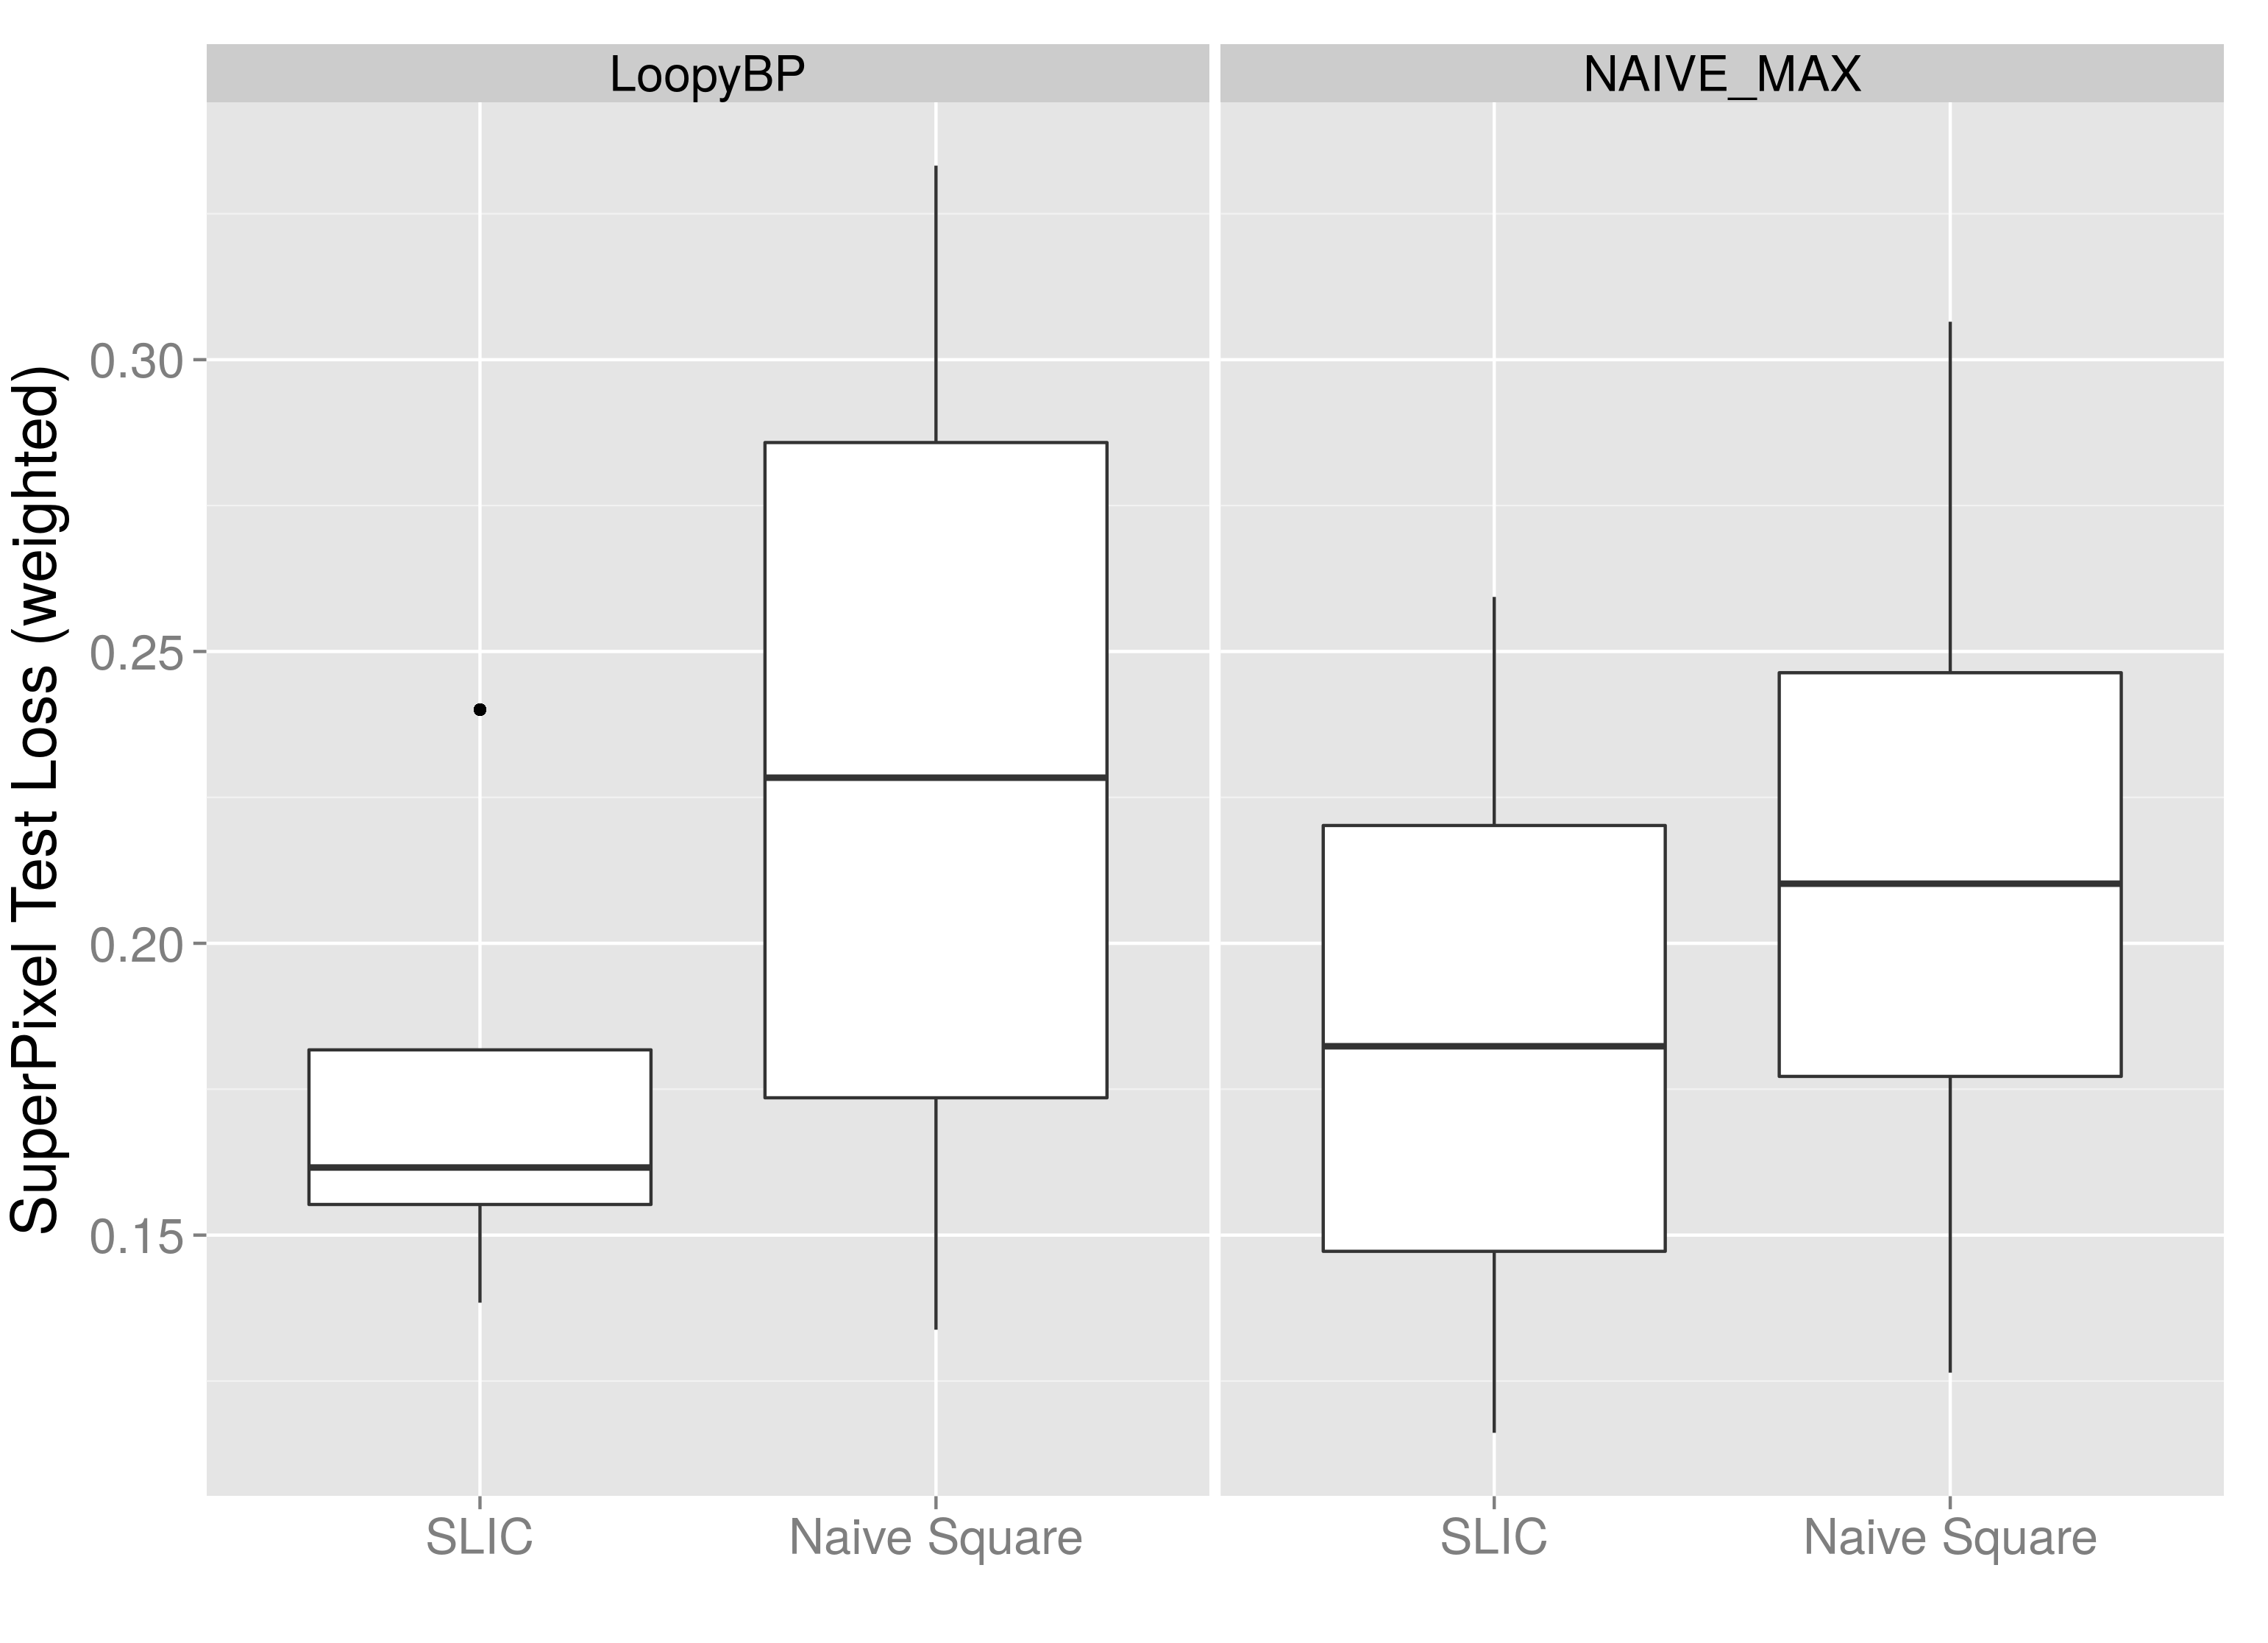
\includegraphics[width=0.8\textwidth]{images/slicVsNaiveSquare_Supx_Nuclei.png}
  \caption{ Comparing the per class frequency per super-pixel test loss using either SLIC or Square super-pixels. The experiment was repeated for Unary model and a Pairwise model solved with Loopy Belief Propagation. Data( Single Channel 3D Nuclei Images \cite{ucsbData}) } 
  \label{fig:slicvssquareNucli}
\end{figure} 
%

\section{Running ScalaSLIC}
ScalaSlic can be used as a standalone package on any kind of data which is saved on spatially located on a uniform grid like color voxels. When constructing a new SLIC() object one needs to input the data in a "Array[Array[Array[DataType]]]" format, where datatype can be an RGB triple, a single grayscale byte but it could also be for example a series of RGB values from a video sequence. While the dataType is technically free from the scala compilers perspective, practically one must be able to define the following functions:  \codeInLine{ distFn:(DataType, DataType) => Double }, which simply measure the distance between two pixels. The functions \codeInLine{rollingAvgFn: ((DataType, DataType, Int) => DataType)} and \codeInLine{normFn: ((DataType, Int) => DataType)} are used for the cluster update step to get an average point in this "DataType" space. For here are the functions we use for RGB  \codeInLine{(a: (Int, Int, Int), b: (Int, Int, Int)) =>  sqrt(Math.pow(a._1 - b._1, 2) + Math.pow(a._2 - b._2, 2) + Math.pow(a._3 - b._3, 2))}, \codeInLine{distFnCol = (a: (Int, Int, Int), b: (Int, Int, Int)) => sqrt(Math.pow(a._1 - b._1, 2) + Math.pow(a._2 - b._2, 2) + Math.pow(a._3 - b._3, 2)) }, \codeInLine{sumFnCol =  (a: (Int, Int, Int), b: (Int, Int, Int)) => ((a._1 + b._1, a._2 + b._2, a._3 + a._3)) } and \codeInLine{normFnCol = (a: (Int, Int, Int), n: Int) => { ((a._1 / n, a._2 / n, a._3 / n))}}. The final mandatory input for ScalaSLIC is \inputArgs{S} which determines the initial grid spacing of the super-pixels and thereby also setting the initial number of cluster centers and partially how large the super-pixels will be. How large the super pixels will be is also modulated by the parameter \inputArgs{M} which specifies the compactness of the super-pixels. If M is not specified we go for the alternative approach of normalizing distances by the max distance in the each super-pixel set. 
\subsection{Visualization SLIC compactness parameters}\label{sec:slicParams}
In our implementation we slightly alter the use of $M$ in contrast to the above distance function. Let $x$,$y$ \& $z$ be vectors containing both pixel coordinates and the spacial centres of the super-pixel clusters index by their subscript. And let $r$, $g$, $b$ be the vectors containing the RGB color information for pixels and super-pixel centres. Here we use subscript $_k$ for some cluster center and subscript $_i$ for some pixel id:   	 $Distance(P,C) = \frac{M^2}{S^2}\sqrt[2]{(x_k -x_i)^2 + (y_k - y_i)^2 + (z_k - z_i)^2} + \sqrt{(r_k - r_i)^2+(g_k - g_i)^2+(b_k - b_i)^2} $. LABColor-space can be used optionally instead of RGB. For an illustration of the effect of parameter $M$ on the segmentation see Figures \ref{fig:showingMonMSRC1}, \ref{fig:showingMonMSRC2} and \ref{fig:showingMonMSRC3}

\begin{figure}[H]
  \centering
  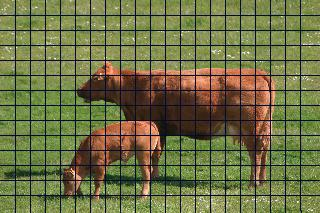
\includegraphics[width=0.7\textwidth,natwidth=610,natheight=642]{images/_supPix_2_15_M0_01_seg.jpg}
  \caption{ SLIC example segmentation on a single 2D MSRC image. With parameters:  S=15, M=1000 } 
  \label{fig:showingMonMSRC1}
\end{figure} 
\begin{figure}[H]
  \centering
  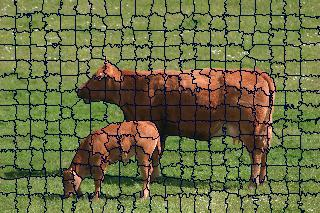
\includegraphics[width=0.7\textwidth,natwidth=610,natheight=642]{images/_supPix_2_15_M5_0_seg.jpg}
  \caption{  SLIC example segmentation on a single 2D MSRC image. With parameters:  S=15, M=45 } 
  \label{fig:showingMonMSRC2}
\end{figure} 
\begin{figure}[H]
  \centering
  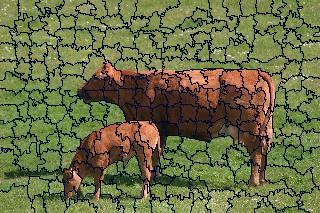
\includegraphics[width=0.7\textwidth,natwidth=610,natheight=642]{images/_supPix_2_15_M10_0_seg.jpg}
  \caption{  SLIC example segmentation on a single 2D MSRC image. With parameters:  S=15, M=14 } 
  \label{fig:showingMonMSRC3}
\end{figure} 

Do to the inherent difficulty of seeing through a block of solid tissue we will visualize the effect of parameter $M$ by only drawing the voxels labelled as foreground, this 3D dataset is a binary classification problem and hence can be displayed like this. 

\begin{figure}[H]
  \centering
  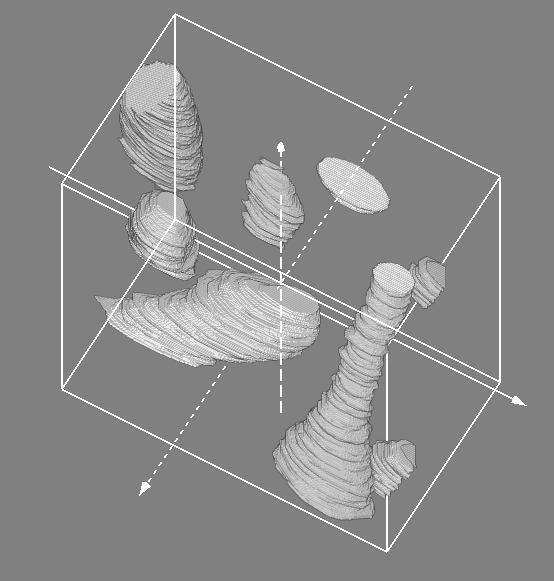
\includegraphics[width=0.7\textwidth]{images/mitochon_groundTruth.png}
  \caption{ The original per pixel ground truth labelling with background transparent and foreground textured to have a surface. Data used in this image is a subset of the EM Mitochondria dataset \cite{mitochondriaData}} 
  \label{fig:showingMmitochonGT}
\end{figure} 
\begin{figure}[H]
  \centering
  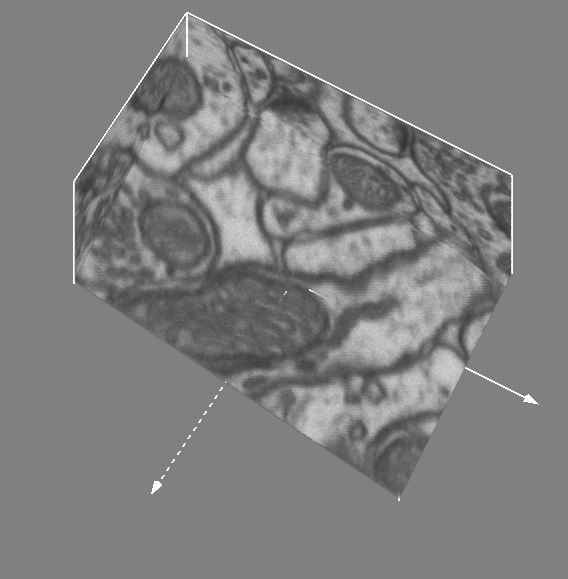
\includegraphics[width=0.7\textwidth]{images/mitochon_original_features.png}
  \caption{ The figure shows a cross sectional cut of the raw data used to construct super-pixels in Figure \ref{fig:showingMmitochonM50} and \ref{fig:showingMmitochonM9}. Data used in this image is a subset of the EM Mitochondria dataset \cite{mitochondriaData}} 
  \label{fig:showingMmitochonRaw}
\end{figure} 

\begin{figure}[H]
  \centering
  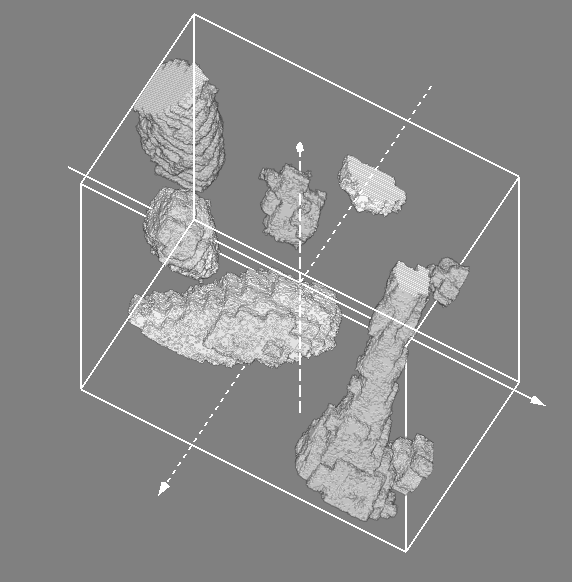
\includegraphics[width=0.7\textwidth]{images/mitochon_s10_m50.png}
  \caption{ The figure shows the textured boundaries of the volume encompassed by the super-pixels which where labelled as being mitochondrial foreground in their graph representation. This image varies from Figure \ref{fig:showingMmitochonM9} in that it used a higher $M=50$The original per pixel ground truth labelling with background transparent and foreground textured to have a surface and hence results in more compact super-pixels. Data used in this image is a subset of the EM Mitochondria dataset \cite{mitochondriaData}} 
  \label{fig:showingMmitochonM50}
\end{figure} 

\begin{figure}[H]
  \centering
  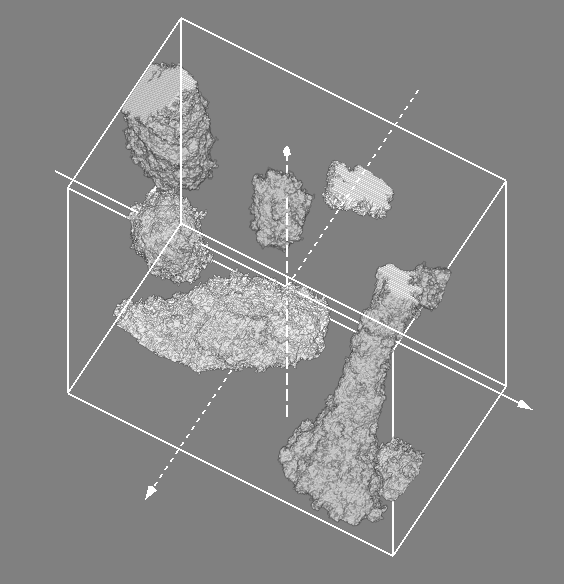
\includegraphics[width=0.7\textwidth]{images/mitochon_s10_m9.png}
  \caption{ The figure shows the textured boundaries of the volume encompassed by the super-pixels which where labelled as being mitochondrial foreground in their graph representation. This image varies from Figure \ref{fig:showingMmitochonM9} in that it used a lower $M=9$ and hence results in less uniformly shaped super-pixels. Data used in this image is a subset of the EM Mitochondria dataset \cite{mitochondriaData}} 
  \label{fig:showingMmitochonM9}
\end{figure} 


%
%
%
%
%

\chapter{Results}
\section{3D Dataset, EM Mitochondria Labelling}
To demonstrate the image segmentation pipeline in all its parts we choose to use a EM Mitochondria dataset because it is a natural dataset with objects which are not easily distinguishable, and still has good labeled data. The single training image of size $1024 \times 768 \times 165$ was split into 82 by 82 by 82 cubes and super-pixels where constructed with $S=10$ and $M=9$ producing a graph with 921 nodes on average. We then trained the Naive Max classifier on a unary model, Mean Field and LoopyBP on a pairwise model and LoopyBP on two data dependent pairwise models. The results show a clear superiority of pairwise models over unary models. Amongst the pairwise models it can be benificial to use a more complex data dependent model but the score variance is too high for a statistically significant difference. Surprisingly we found that with a $\lambda =100$ Mean Field performed close to LoopyBP with lower training time. See Figure \ref{fig:mitochonCmpMethods} for details. 


\begin{figure}[H]
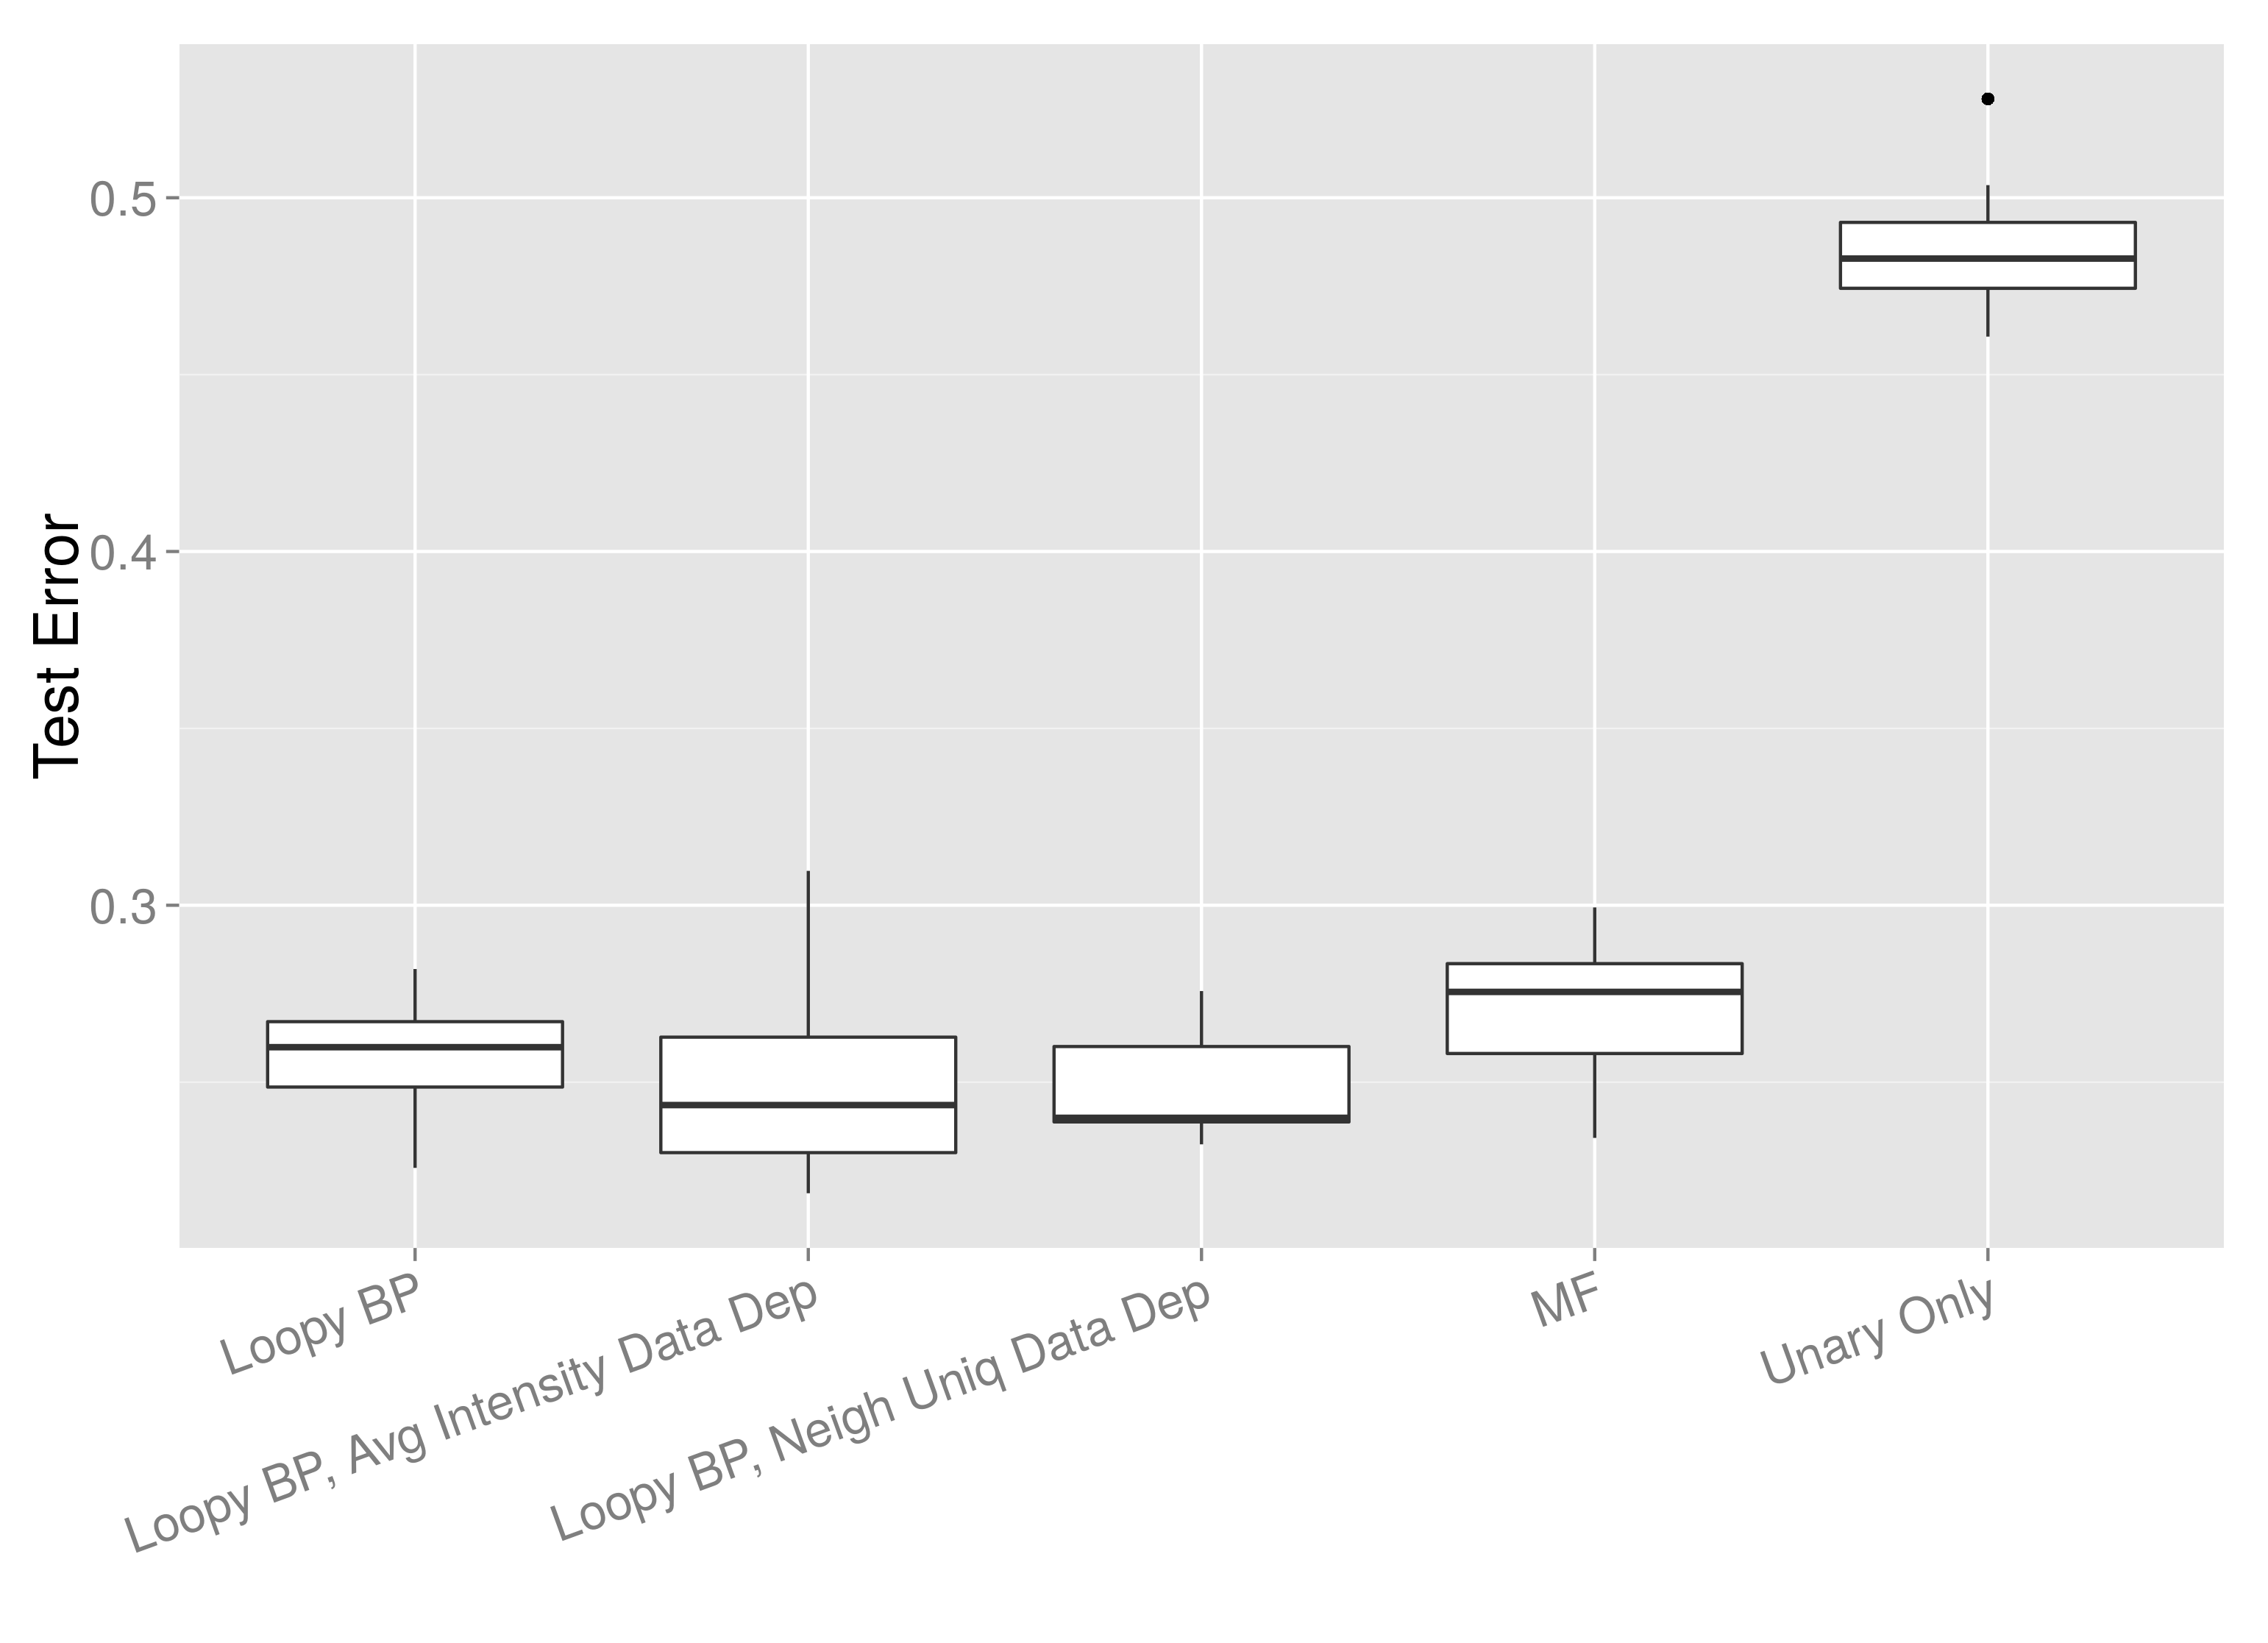
\includegraphics[width=0.8\textwidth]{images/mitochonSplit_testError_end.png}
  \caption {  Over 30 rounds we trained the SSVM with different using different models and different max oracle functions. LoopyBP and MF where trained on a simple pairwise model as in \ref{sec:pariwiseSimple}. Naive Max oracle was trained a Unary only model see \ref{sec:unaryModel}. Additionally we trained two data dependent pariwise models (see section \ref{sec:dataDep}) with LoopyBP max-oracle. The data dependent pairwise transition binning function "Avg Intensity" groups neighbouring nodes by the difference in the mean intensity inside each super-pixel, the function "Neigh Uniq" calcluates how many standard deviations away the mean of node A is from the distribution of intensities in the one hope neighbourhood of node B. Data:( EM Mitochondira Labeled Image split into $82^3$ cubes with super-pixels of size $S=10$ \cite{mitochondriaData} ) } 
  \label{fig:mitochonCmpMethods}
\end{figure}


\section{Sparse Transition Probability Tables}
During our exploration of different datasets we saw high variance on whether the pairwise models increases accuracy as compared to the baseline naive unary max oracle. To examin which situations the pairwise term is particularly helpful we designed as set of synthetic experiments. For details on the data generation functions see Appendix \ref{sec:synthDataGen}. In the following experiments we generated data with a significant amount of noise and set rules for how many labels are allowed to be adjacent to any label A for all other labels. We call the probability that two labels are allowed to be neighbours \inputArgs{dataGenNeighProb}. If we were to allow any label to be next to any other label then the only thing the pairwise term can learn is that super pixels generally occure in groups. So they are generally more likely to occur next to one of their own label versus any other. But by restricting only few labels to be allowed as neighbours we give the pairwise term a target which contains many zeros and hence will have a greater impact on the decoding energy. In the following graph we show the accuracies of pairwise versus unary model while changing the probability that any 2 classes are allowed to be neighbours.

\begin{figure}[H]
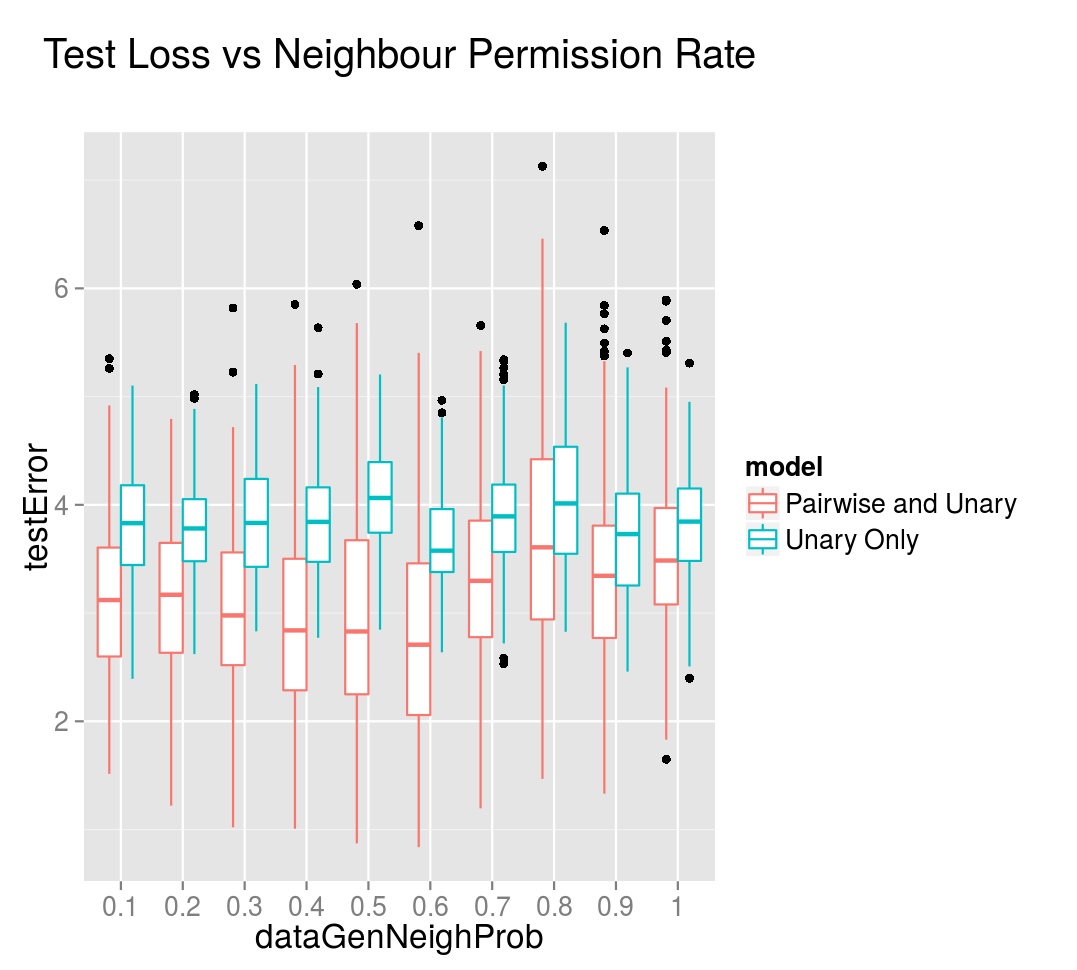
\includegraphics[width=1\textwidth]{images/tesLoss_vs_Neighbour_permission.png}
  \caption { As the \inputArgs{datagenNeighProb} decreases it creates a more sparse transition probability matrix which makes it easier for the pairwise models to identify this information. Once below 0.3 the pairwise benefit starts decreasing again because the likelihood of the most of the image being the background label increases. Data ( SynthData, WhiteNoise:0.40 SquarImgSize:30 OsilNoise:0.40 SupSqrColorShift:0.0 SuperPix, S:5, M:5, Max Decoding:LoopyBP ) } 
  \label{fig:neighprobVSloss}
\end{figure}

As the reader can see the largest difference between unary and pairwise occurs in the middle of the graph. This is because as \inputArgs{dataGenNeighProb} goes to 1.0 all classes can be adjacent to all others. As it approaches 0.0 the image becomes mostly background because that label is reserved as a fallback when all other labels are not allowed due to the neighbouring rules. In Table \ref{table:neigh1} the reader can inspect columns of the transition probability and the weights learned in the pariwise model for data using this transition probability table. Notice, those label pairs which have the highest transition probability also have the highest weight in the corresponding learned pairwise potential column. In contrast table \ref{table:neigh2} does not have this correspondence. BCFW does not have an objective of learning the correct transition probabilities but rather to decrease the hinge loss. For this objective it only alters the direction of $\weightVect$ if that portion of the feature vector is usefull in destingushing data. Hence when the transition probability is not sufficiently distinguishable between images it will not be learned. 
\begin{table}
\caption{Transitions tables using \inputArgs{dataGenNeighProb=0.4} }
\label{table:neigh1}
\subcaption*{True Transition probability between labels}
\centering
\begin{tabular}{ c c c c}
	0.000e+00 &	4.245e-01 & 3.271e-02 &	0.000e+00 \\
	4.245e-01 &	0.000e+00 &	2.861e-02 &	0.000e+00 \\
	3.271e-02 &	2.861e-02 &	1.667e-03 &	1.333e-02 \\
	0.000e+00 &	0.000e+00 &	1.333e-02 &	0.000e+00 \\
\end{tabular}
\bigskip
\subcaption*{Learned Pairwise Weights}
\begin{tabular}{ c c c c}
  -7.349e-04 & 4.557e-04 & 3.112e-04 & -2.030e-05 \\
  4.557e-04 & -1.305e-04 & -3.408e-04 & -1.313e-04 \\
  3.112e-04 & -3.408e-04 & -1.149e-04 & 1.250e-04 \\
  -2.030e-05 & -1.313e-04 & 1.250e-04 & -5.570e-05 \\
\end{tabular}
\end{table}
\begin{table}
\caption{ Transition tables using \inputArgs{dataGenNeighProb=1.0}: }
\label{table:neigh2}
\subcaption*{True Transition probability between labels}
\centering
\begin{tabular}{ c c c c}
  1.046e-01 & 1.106e-01 & 1.120e-01 & 2.292e-03 \\
  1.106e-01 & 1.061e-01 & 1.099e-01 & 2.500e-03 \\
  1.120e-01 & 1.099e-01 & 1.092e-01 & 2.778e-03 \\
  2.292e-03 & 2.500e-03 & 2.778e-03 & 1.389e-04 \\
\end{tabular}
\bigskip
\subcaption*{Learned Pairwise Weights} 
\begin{tabular}{ c c c c}
  7.650e-05 & 3.878e-04 & 2.306e-04 & 4.022e-05 \\
  3.878e-04 & 2.015e-04 & 3.430e-04 & 4.590e-05 \\
  2.306e-04 & 3.430e-04 & -7.471e-05 & 3.638e-05 \\
  4.022e-05 & 4.590e-05 & 3.638e-05 & -4.405e-05 \\
\end{tabular}

\end{table} 
With the sparse transition probability explanation for the pairwise advantage in mind we can construct a dataset which should give more advantage to the pariwise model by making the super-pixels exactly equal to the supersquares. This configuration should result in transition probabilities from the label to itself (the diagonal) being as sparse as the rest of the matrix. In Figure \ref{fig:s_equals_superSquare} we see the expected result, that the distance between the pairwise and unary model increases as we farther increase the sparsity of the transition probability matrix. 


\begin{figure}
\centering
\caption{Test Error vs Label Transition Sparsity}
\subcaption*{With Superpixel size == SuperSquare size}
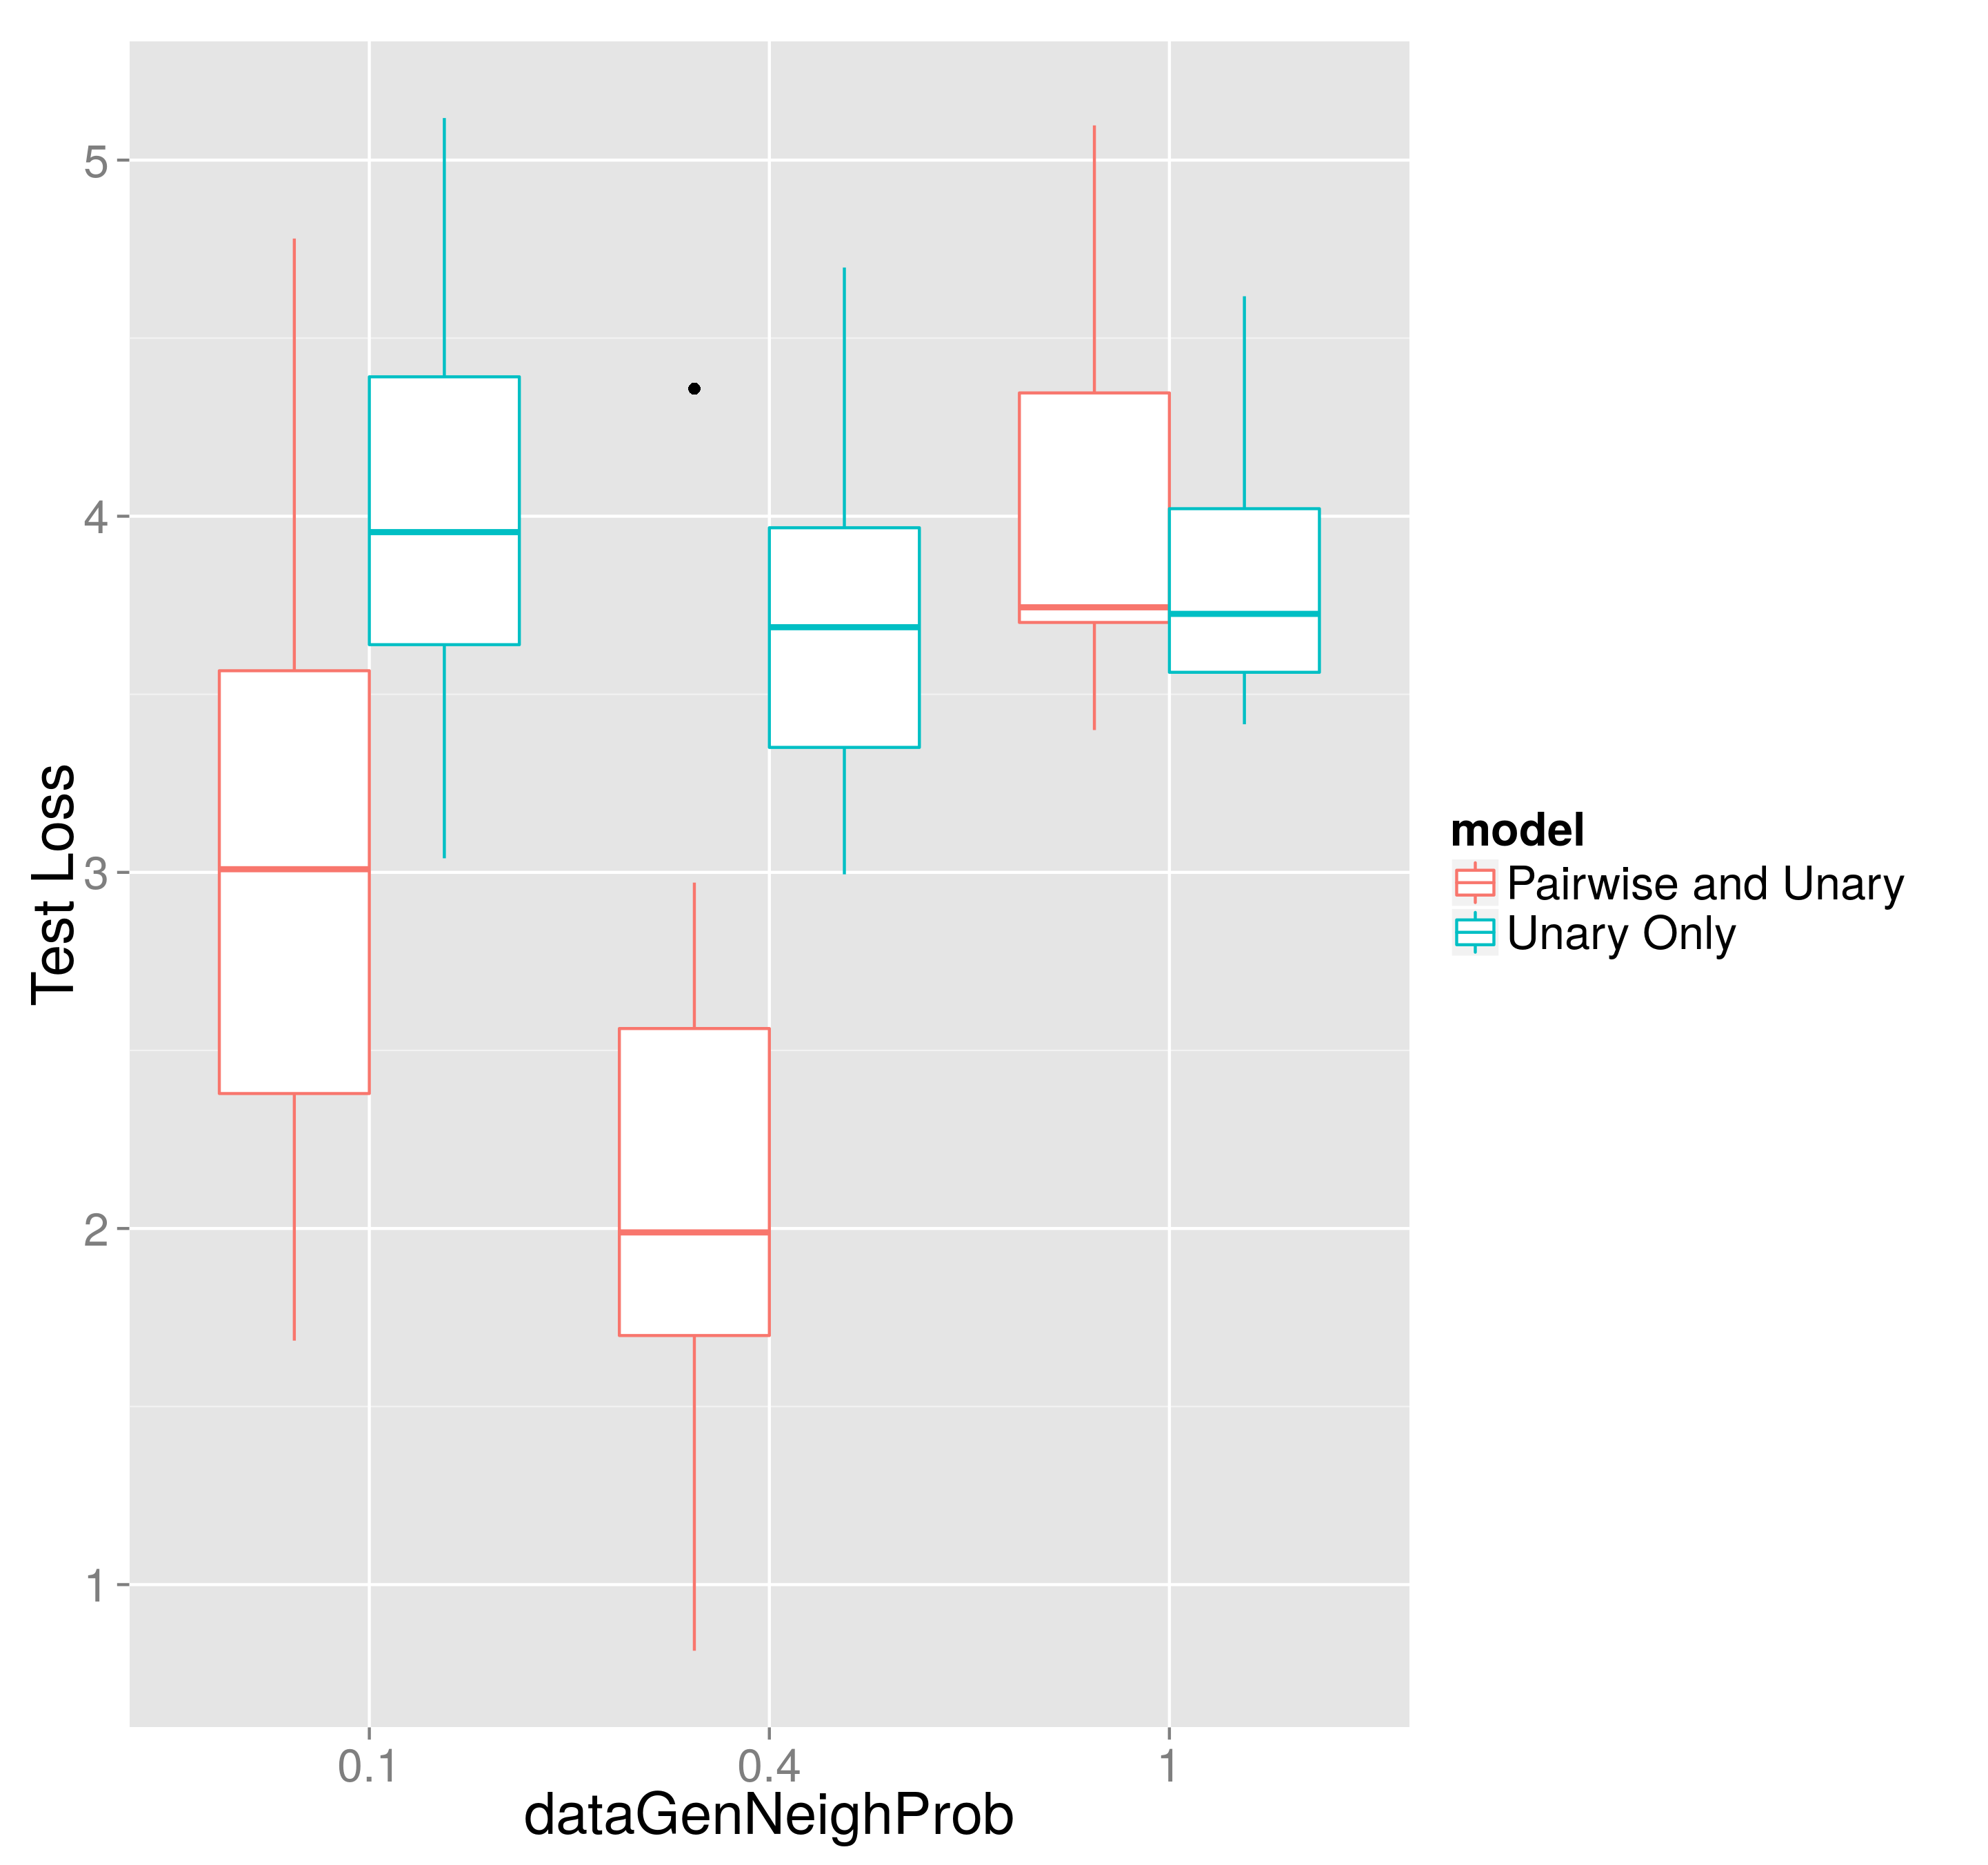
\includegraphics[width=1.0\textwidth]{images/neighProb_s_equals_supSquare.png}
\caption{ The figure shows a substantial improvement in the test Error for the pairwise model. These results can be compared to \ref{fig:neighprobVSloss} which is the same experiment but with smaller super pixels. Since in this experiment we set the superpixels equal to the supersquare size the diagonal of the transition probability matrix is just as sparse as the rest.  Data ( SynthData, WhiteNoise:0.40 SquarImgSize:30 OsilNoise:0.40 SupSqrColorShift:0.0 SuperPix, S:30, M:30, Max Decoding:LoopyBP ) }
\label{fig:s_equals_superSquare}
\end{figure}


\section{Prediction Smoothing}\label{smoothness}
By visual inspection of label predictions we subjectively observed a trend of the pairwise models performing better when disconnected single lables in clusters of others labels is unlikely. 
In figure \ref{fig:smooth1} we can see the upper row of predicted labels by the pairwise model is much smoother than the lower row of unary model predictions.  As described above the supersquares are always of equal size and in this configuration contain several superpixels internally. The image is not perfeclty smoothed into squares because we jointly optimize pairwise and unary factors. 
Figure \ref{fig:smoothNuclie} gives evidence for the same understanding of smoothness as figure \ref{fig:smooth1} but with real world data. Again we see that the pairwise model has less standalone super pixel labels indicating that the pairwise term is working as expected. But in this particular experiment the the pairwise term also had a negative effect as on the lower side of the nuclei cluster is another set of high contrast objects which are only slightly disconnected from the main body. These nearby easily mistaken objects are all grouped into the main nuclei cluster in using the pairwise term resukt in a worse score than the few misslabeling made by the unary model. Hence we must be mindful of the way in which we are including the spacial relations into our model, as in this datasets where one must consider that there may be a separation between groups of classes which is less than one super pixel wide. One way to combat this could be to set the compactness parameter for the SLIC preprocessing very low so that thin long superpixels could be placed between the two groups of classes. 
\begin{figure}[H]
  \centering
  
  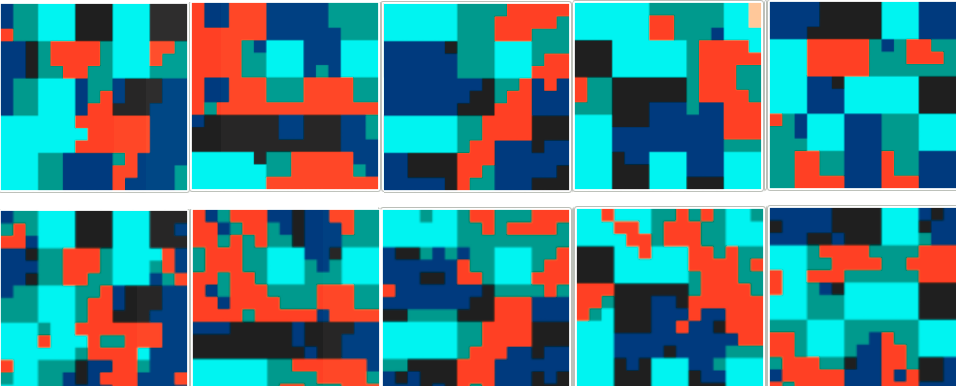
\includegraphics[width=0.8\textwidth]{images/compare_smoothness_syntheticData_pariwise_v_unary.png}
  \caption{ This figure shows the predicted labels per pixel for a pairwise model in the top row and a unary only model in the bottom row. By visual inspection the reader can see that the top pairwise model is more smooth in that the blobs of labels are more connected and generally in larger collections. While the bottom unary model output frequently has a single super pixel with a label surrounded by larger groups of distinct labels. Data ( SynthData, WhiteNoise:0.40 SquarImgSize:30 OsilNoise:0.40 SupSqrColorShift:0.0 SuperPix, S:30, M:30, Max Decoding:LoopyBP/NiveMax )} 
  \label{fig:smooth1}
\end{figure} 
\begin{figure}
\begin{subfigure}{.5\textwidth}
  \centering
  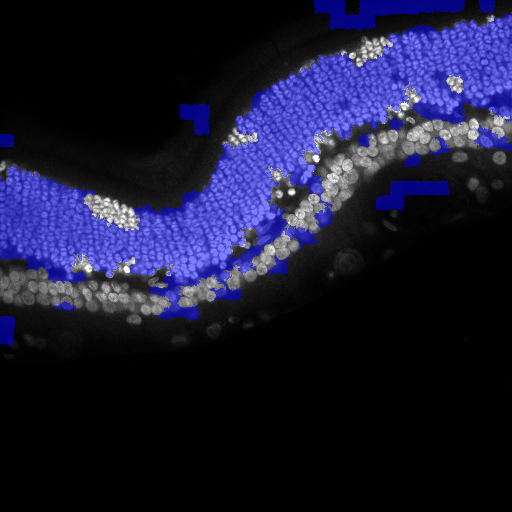
\includegraphics[width=0.9\linewidth]{images/3dnone_0-train_predict_unary.png}
  \caption{Unary Model prediction}
  \label{fig:smoothNuclieUnary}
\end{subfigure}%
\begin{subfigure}{.5\textwidth}
  \centering
  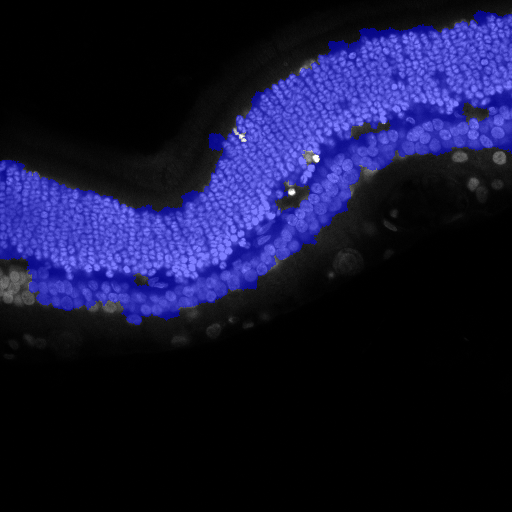
\includegraphics[width=0.9\linewidth]{images/3dnone_0-train_predict_pairwise.png}
  \caption{Pairwise Model prediction}
  \label{fig:smoothNucliePair}
\end{subfigure}
\caption{ Per-superpixel predicted labels are superimposed on the raw image. This Nuclei detection dataset only has foreground and background hence we only colored the Nuclei label foreground predictions. The reader can observe that the Unary model (a) has more disconnected components than the Pairwise model (b). In this particular dataset the nuclei are always connected in one large object hence giving pairwise model an advantage to not make this kind of error. Data( Single Channel 3D Nuclei \cite{ucsbData}) }
\label{fig:smoothNuclie}
\end{figure}
\section{Impact of the Regularizer }\label{sec:Lambda}
Out of all the tuning parameters \inputArgs{lambda} needs to be adjusted most carefully, as it determines the freedom $W$ has. In the optimization function $\lambda$ can be interpreted as weighing the size of the margin and the actual loss defined in the slack variable (see equation \vref{optimizationFunc}). As we can see in figure \ref{fig:lambda1} choosing the right lambda for your problem is crucial for the final outcome. This pattern in test error can be further explained when looking at the structured hinge loss over rounds, Figure \ref{fig:lambda2}. We can see that for low lambdas the Structured Hinge loss $\shloss$ does not decrease over meaning that the lambda was so restrictive on the norm of $\weightVect$ that BCFW could not find a piece of information which was usefull enough to warrent changing the norm of $\weightVect$. 

\begin{figure}
  \centering
    \figuretitle{ Test Error vs Lambda, Using Untransformed Features}
  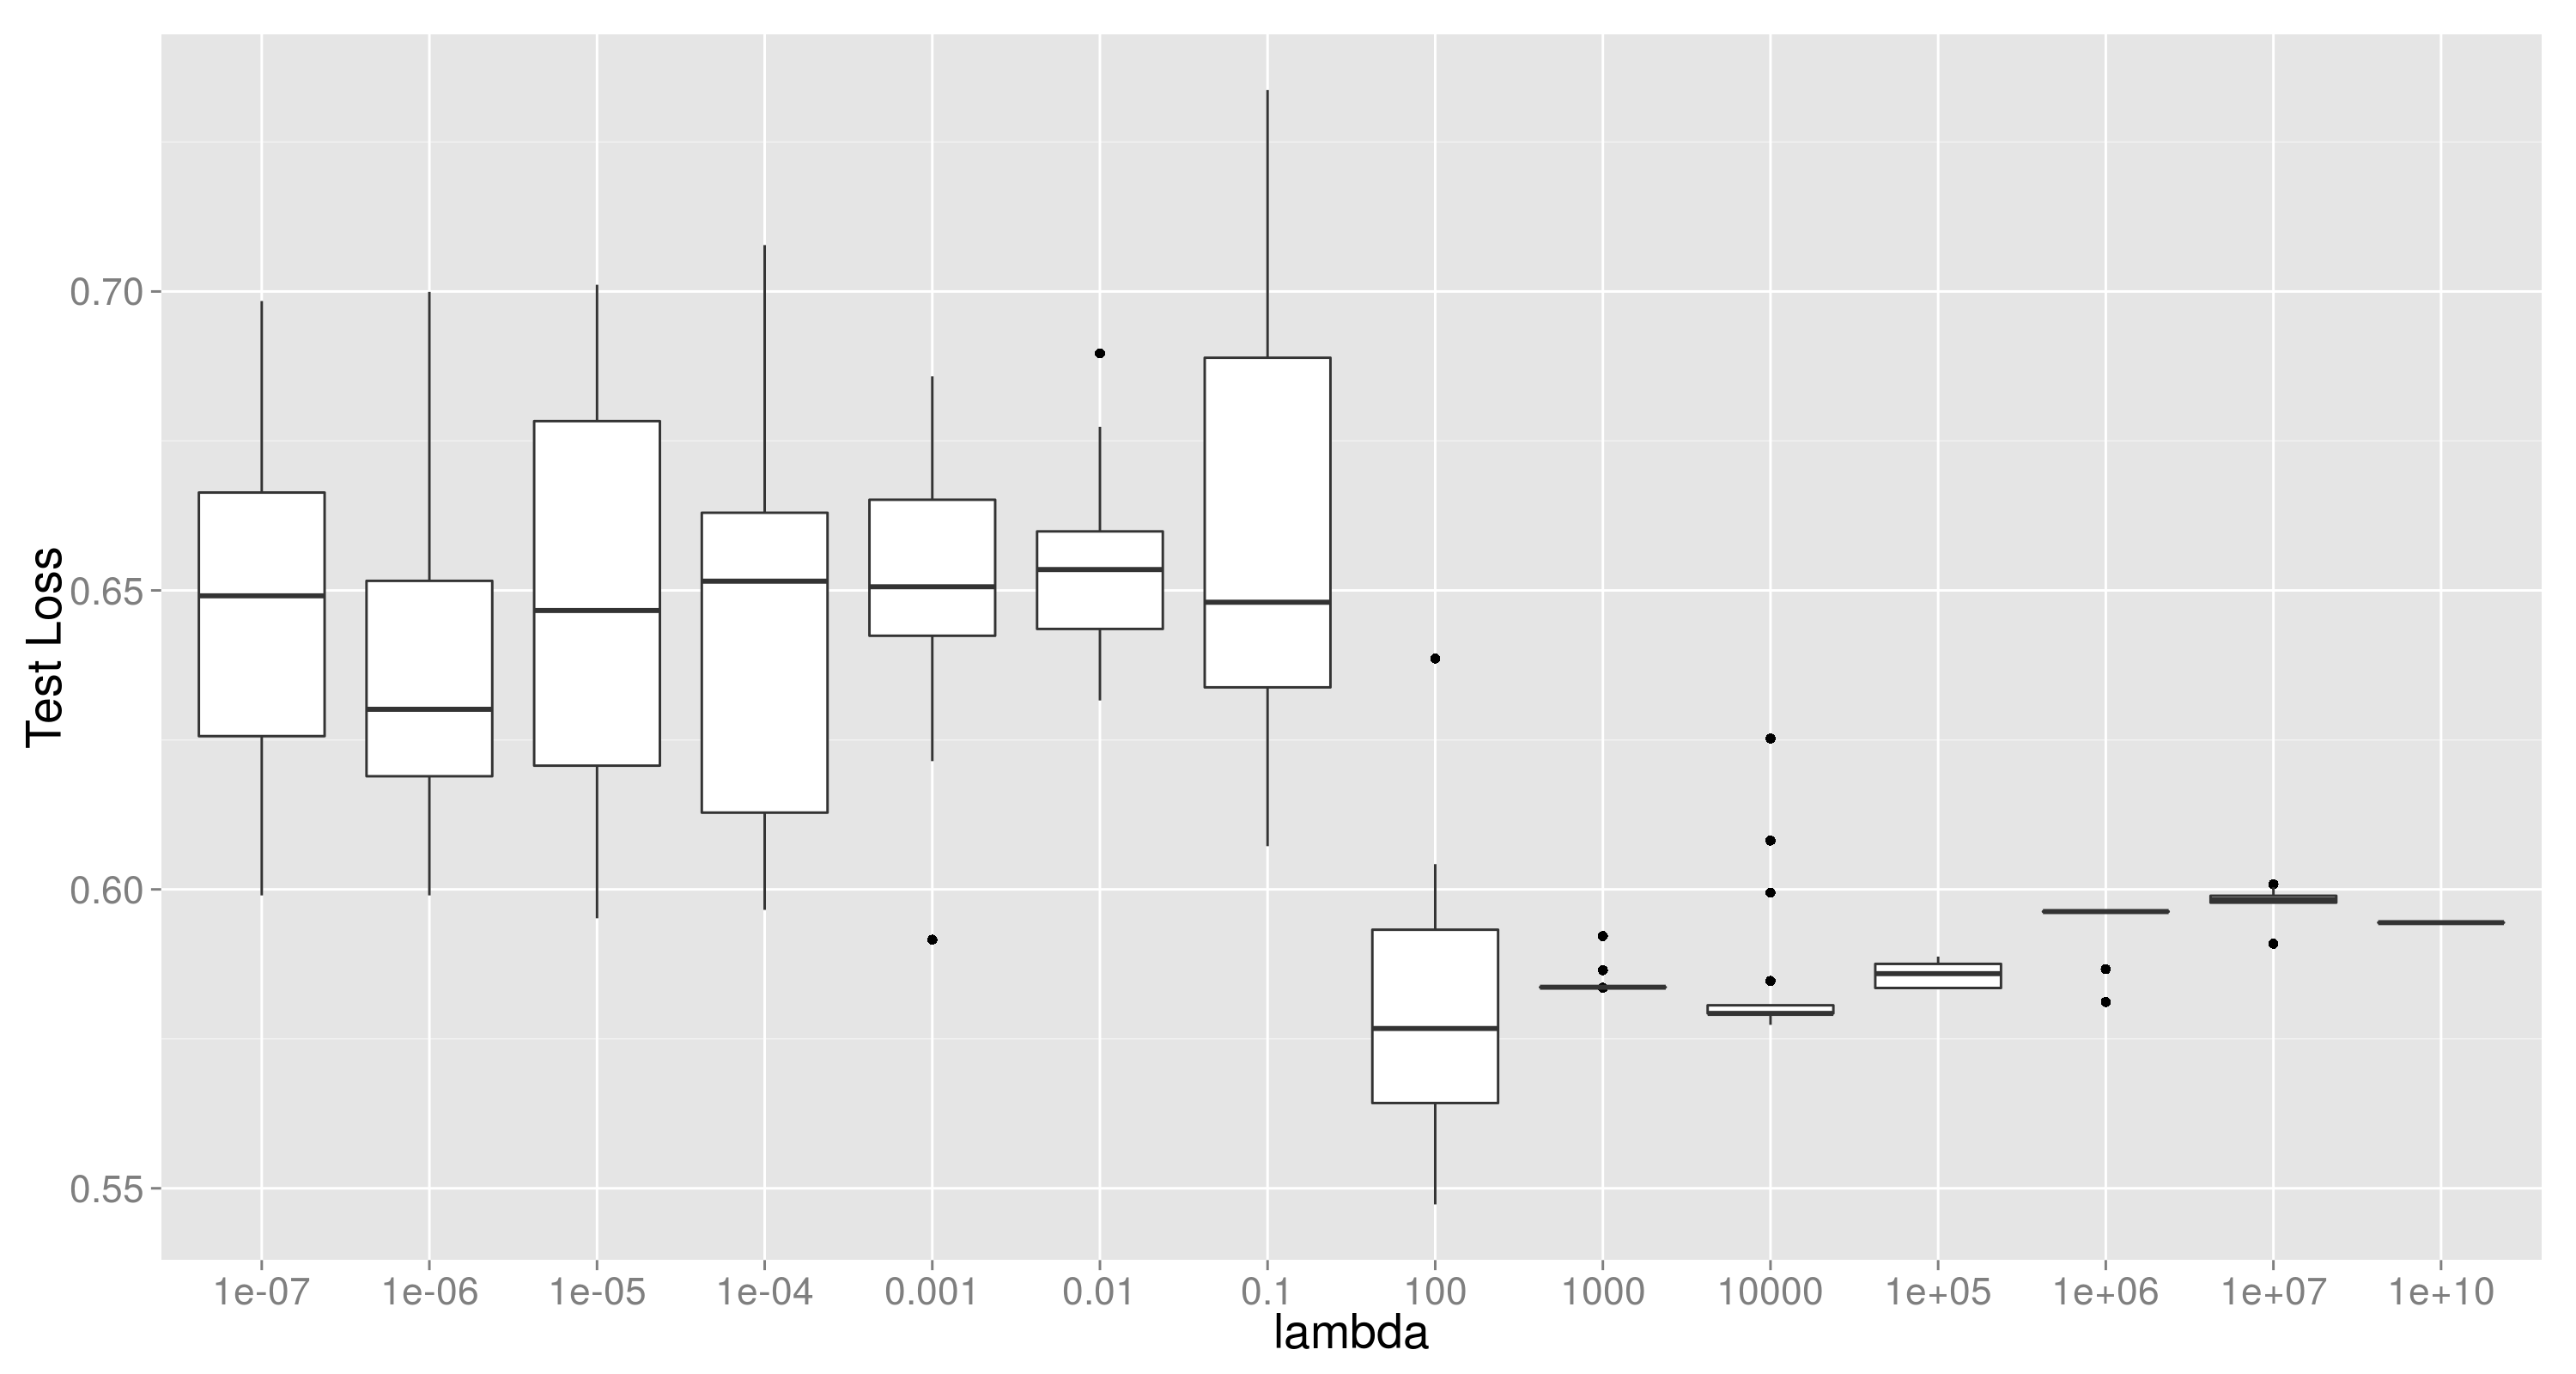
\includegraphics[width=1.0\textwidth]{images/tesatError_vs_lamda_msrc.png}
  \caption{   Displayed are the test scores of the same model run with different regularization lambdas. The distribution displayed was produced by insample cross validation. We can see a clear separation between lambdas which are not strict enough to result in good convergence ($\geq 100, \leq 10000$) and those which do not converge ($\leq 0.1$). Additionally lambdas which are too strict result in lower accuracy again do to them not allowing full exploration of the relations between the features ($\geq 100000$). Data( MSRC version 2 \cite{msrcDataSet}) } 
  \label{fig:lambda1}
\end{figure} 

\begin{figure}
  \centering
  \figuretitle{Structured Hinge Loss over time, faceting on different lambdas}
  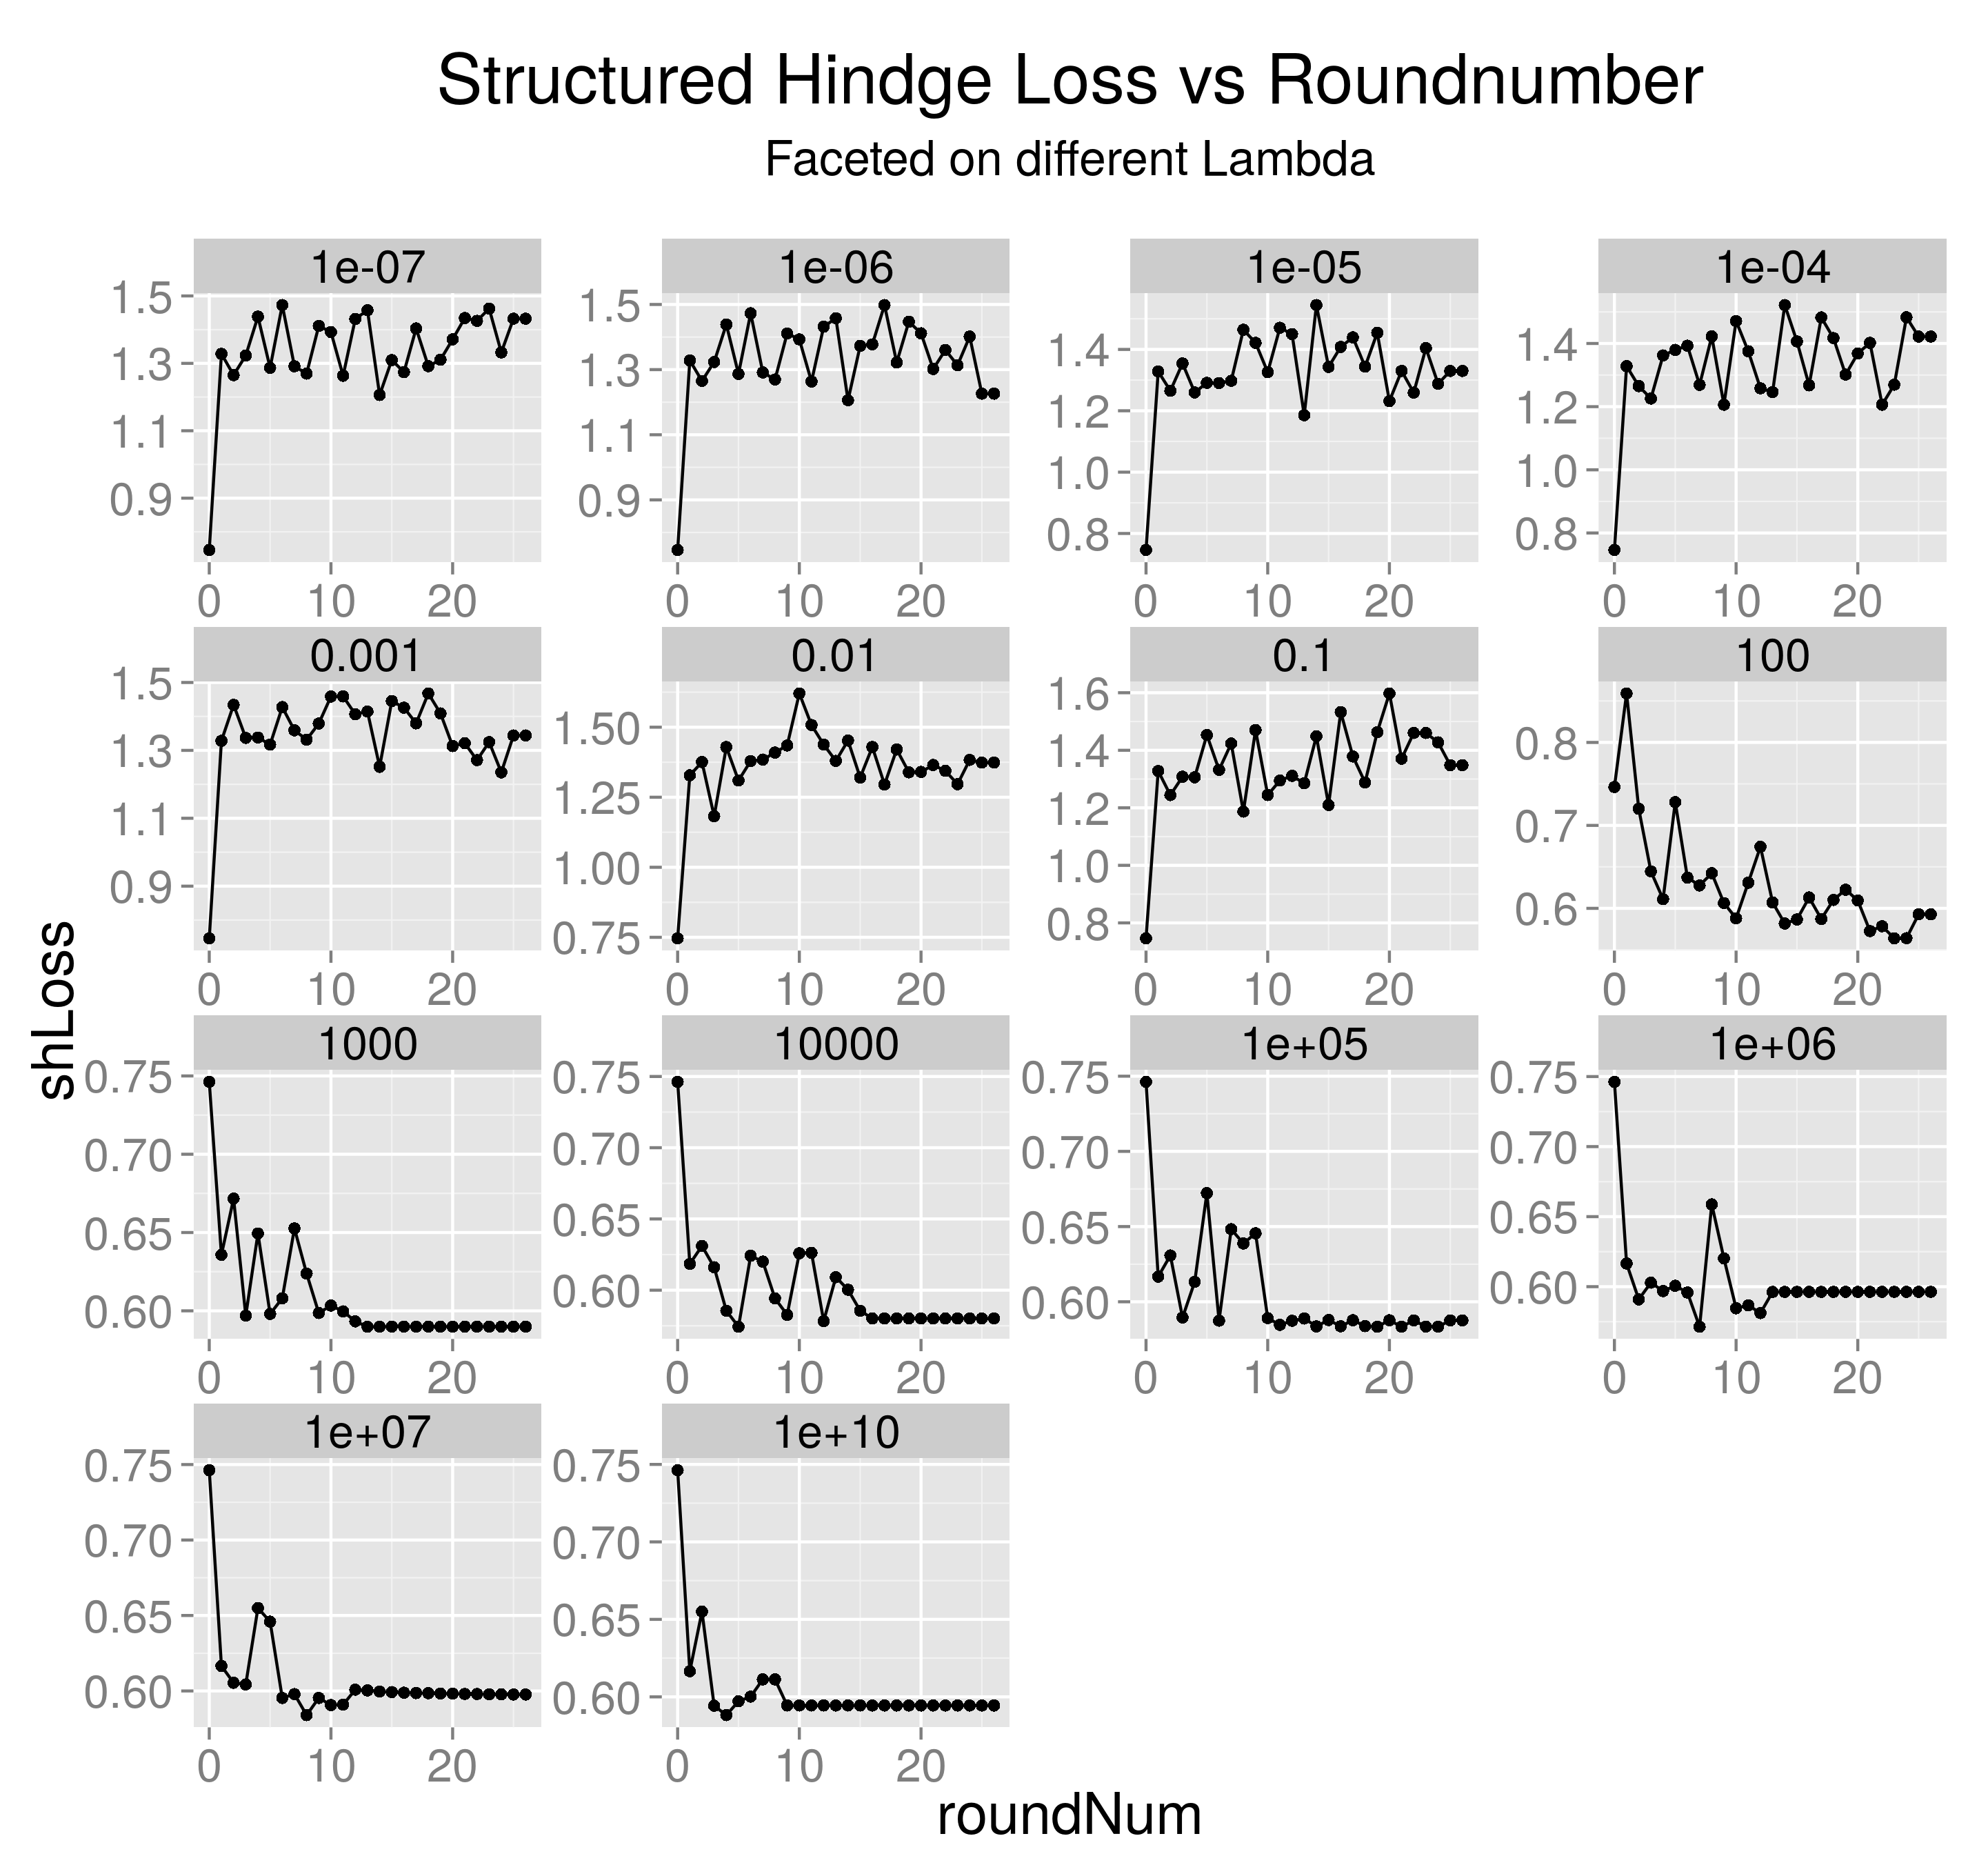
\includegraphics[width=0.8\textwidth]{images/structuredHindgeLoss_vs_lambda_per_Round_msrc_subset.png}
  \caption{This Figure shows the Structural Hinge Loss $\shlossexp$ over time varying the regulerization paramater lambda.  A clear difference can be seen between low lambdas up to 0.1 which do not have a negative trend and also do not seem to converge in terms of structured hinge loss, while lambdas 100 and above have a clear negative trend over time and as lambda gets larger they also converge faster. It should be noted that each experiment starts with the same $w$ and hence also starts with the same structured hinge loss of 0.7462. Data( MSRC version 2 \cite{msrcDataSet}) 	 } 
  \label{fig:lambda2}
\end{figure} 

\begin{figure}
  \centering
  \figuretitle{ Test Error vs Lambda, Using Standardized Features}
  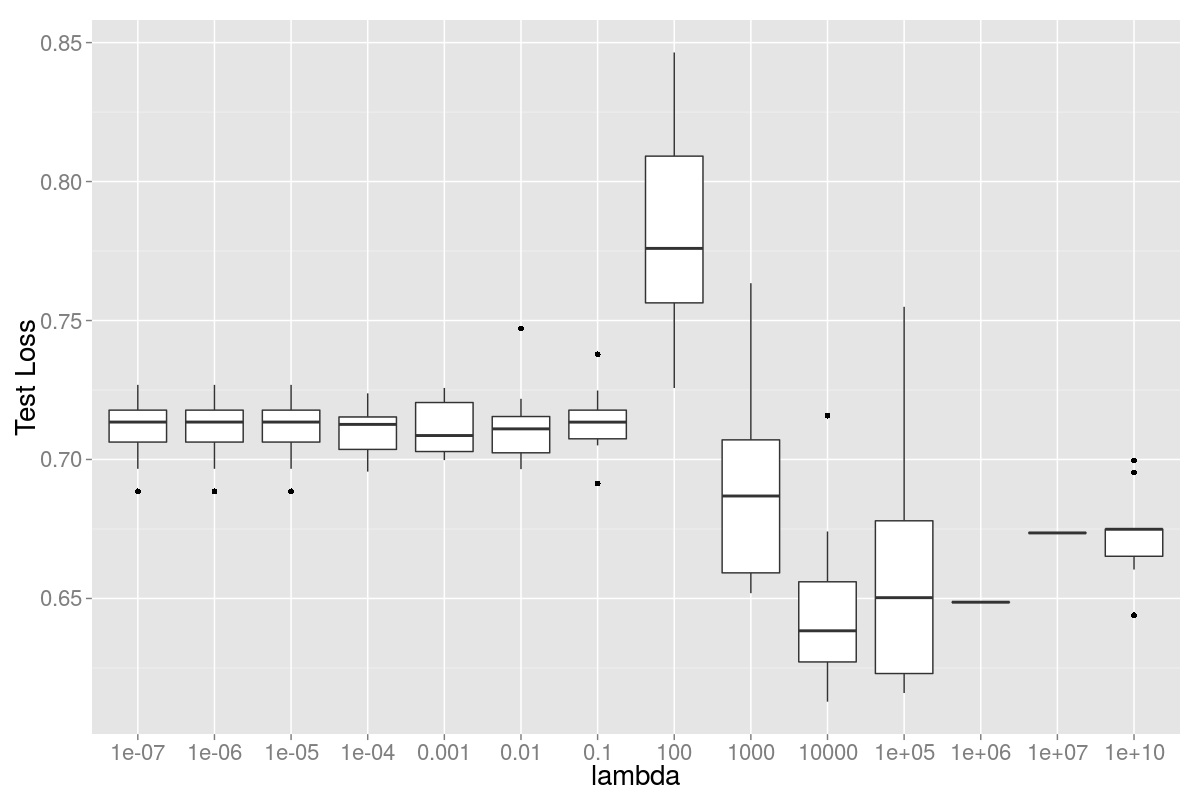
\includegraphics[width=1.0\textwidth]{images/testError_vs_lambda_msrc_stdON.png}
  \caption{  Similar to Figure \ref{fig:lambda1} we can see that low lambdas do not converge properly and hence have significantly higher loss. In this experiment the lowest loss is at 100000 several orders of magnitude higher than in Figure \ref{fig:lambda1} which ran the same experiment only changing the  feature standardization setting.; Data( MSRC version 2 \cite{msrcDataSet} ) 	 } 
  \label{fig:lambdaSTD2}
\end{figure}
\par
To gain farther understanding about the effect lambda has on convergence we can consider the effect it has on the $norm(w)$ over time. See Figure \ref{fig:lambdaWnormNucl1} which shows us how the norm of $w$  does not converge with a lambda of 100 and below but as lambda is increased we can see the curvature also increases indicating it would converge faster with higher lambdas. The test scores with really low lambda are not good but they are still significantly better than pure chance labeling, this can be explained when considering that as lambda goes to zero the optimization problem becomes a simple structured perception which still has the ability to learn a decision boundary but it of course has very poor generalizability as can be seen by the high variance in the score between rounds in Figure \ref{fig:lambdaTestNucl2}. 
\par
Lambda 1000 has a nice shape showing in early rounds $w$ is changing significantly from its initialization of zero and then the norm increase plateauing indication the model has reached some kind of a stable point. Although the $norm(w)$ can appear to be staying constant while the direction of $w$ changes continuing to improve accuracy. Still since we change $w$ in incremental steps such a curve as with lambda=1000 is indication of a good choice. This choice of lambda can be confirmed if one calculates the test error every round as in Figure\ref{fig:lambdaTestNucl2} and we observe a decreasing trend over successive rounds. 
\par
Lambdas greater than or equal to 10000 make their initial move away from zero in the first round but then steadily decrease until plateauing. One would expect that this strange kind of behavior would not result in any reasonable solution but it turns out if we look at Figure\ref{fig:lambdaTestNucl2} that the test error for the highest lambda is actually very close to the best solution found at $\lambda=1000$. To explain this behavior consider the dual objective $\dualObj$ where $\dualA$:=$\dualAexp$ and  $\dualb$:=$\dualbexp$, with very high lambdas the first term of the dual would drop out due to the squared $\dualA$ with a $\lambda$ in the denominator ( $\dualObjLimitLambda$). Now we can see that with high lambdas solving the dual would end up optimizing for the point which would have the highest loss for each $\ySpace$ individually such that $\alpha_i(y^\ast)=1$ where $argmax_{y^\ast}\lossFn(y^\ast) $ and $\alpha_i(y^\prime)=0, \forall y^\prime \neq y^\ast$ since $\alpha$ is constraint with $\dualObjConst$. With KKT conditions $w=\dualA \alpha$ is simply the sum of the joint features maps of the most violating label configurations for each datapoint. If we where to consider this solution in the special case of the binary SVM $w$ would be the vector which if extended would go through the centroid of both classes. The figures used in this section where based on data which was infact binary \cite{ucsbData} and if we look at Figure \ref{fig:lambdaSTD2} which used the MSRC dataset with 24 labels the high lambda solutions are much farther away from the optimal than with binary labeled data.
\par




\begin{figure}
  \centering
  \figuretitle{ Norm(W) over rounds, faceting Lambdas}
  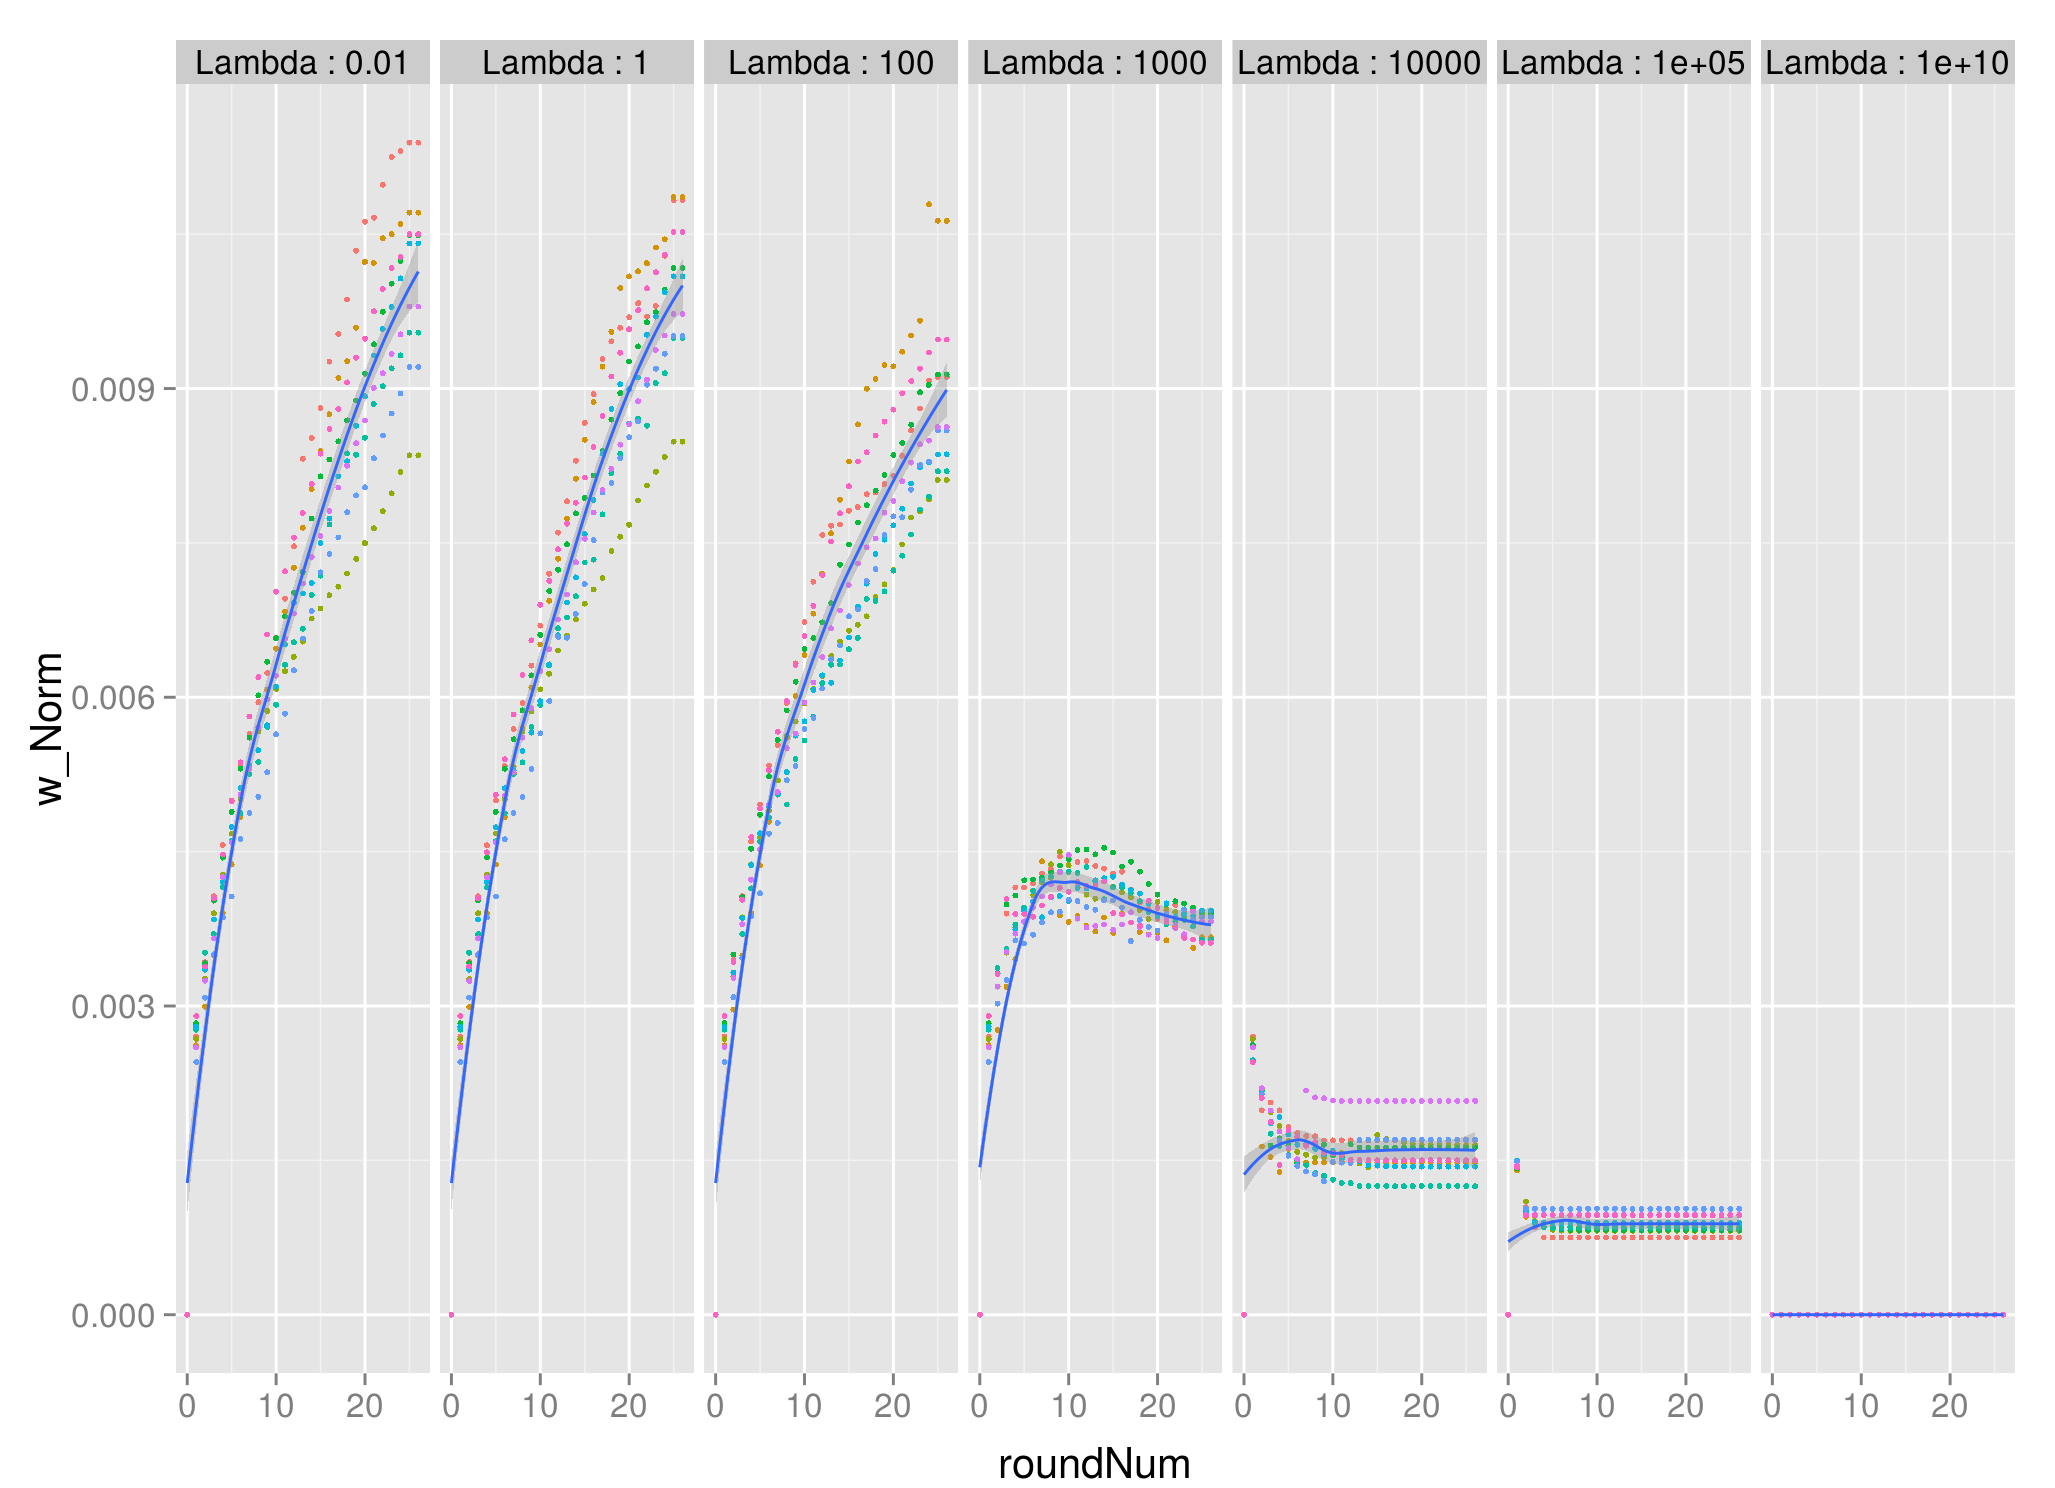
\includegraphics[width=1.0\textwidth]{images/wNorm_nuclei_equalScale.png}
  \caption{ The change in the Norm of the weight vector $\weightVec$ over time is a good indicator of the algorithms convergence depending on lambda. When Lambda is 1 the augmented hinge loss will prefer the $\weightVect$ which has the smallest amount of loss, once the loss can not be improved significantly anymore it will start to choose $\weightVect$ with a larger margin (Large Margin and Low Norm are equivalent in the SVM). The smaller $\lambda$ gets the longer the algorithm can optimize the loss without worrying about the margin. If Lambda where zero then we would have a simple perceptron. When lambda becomes too large the norm curve of $\weightVect$ does not have the expected trend but one can still see if the algorithm converged. Data( Single Channel 3D Nuclei \cite{ucsbData}) } 
  \label{fig:lambdaWnormNucl1}
\end{figure}

\begin{figure}
  \centering
  \figuretitle{ Test Error over rounds, faceting Lambdas}
  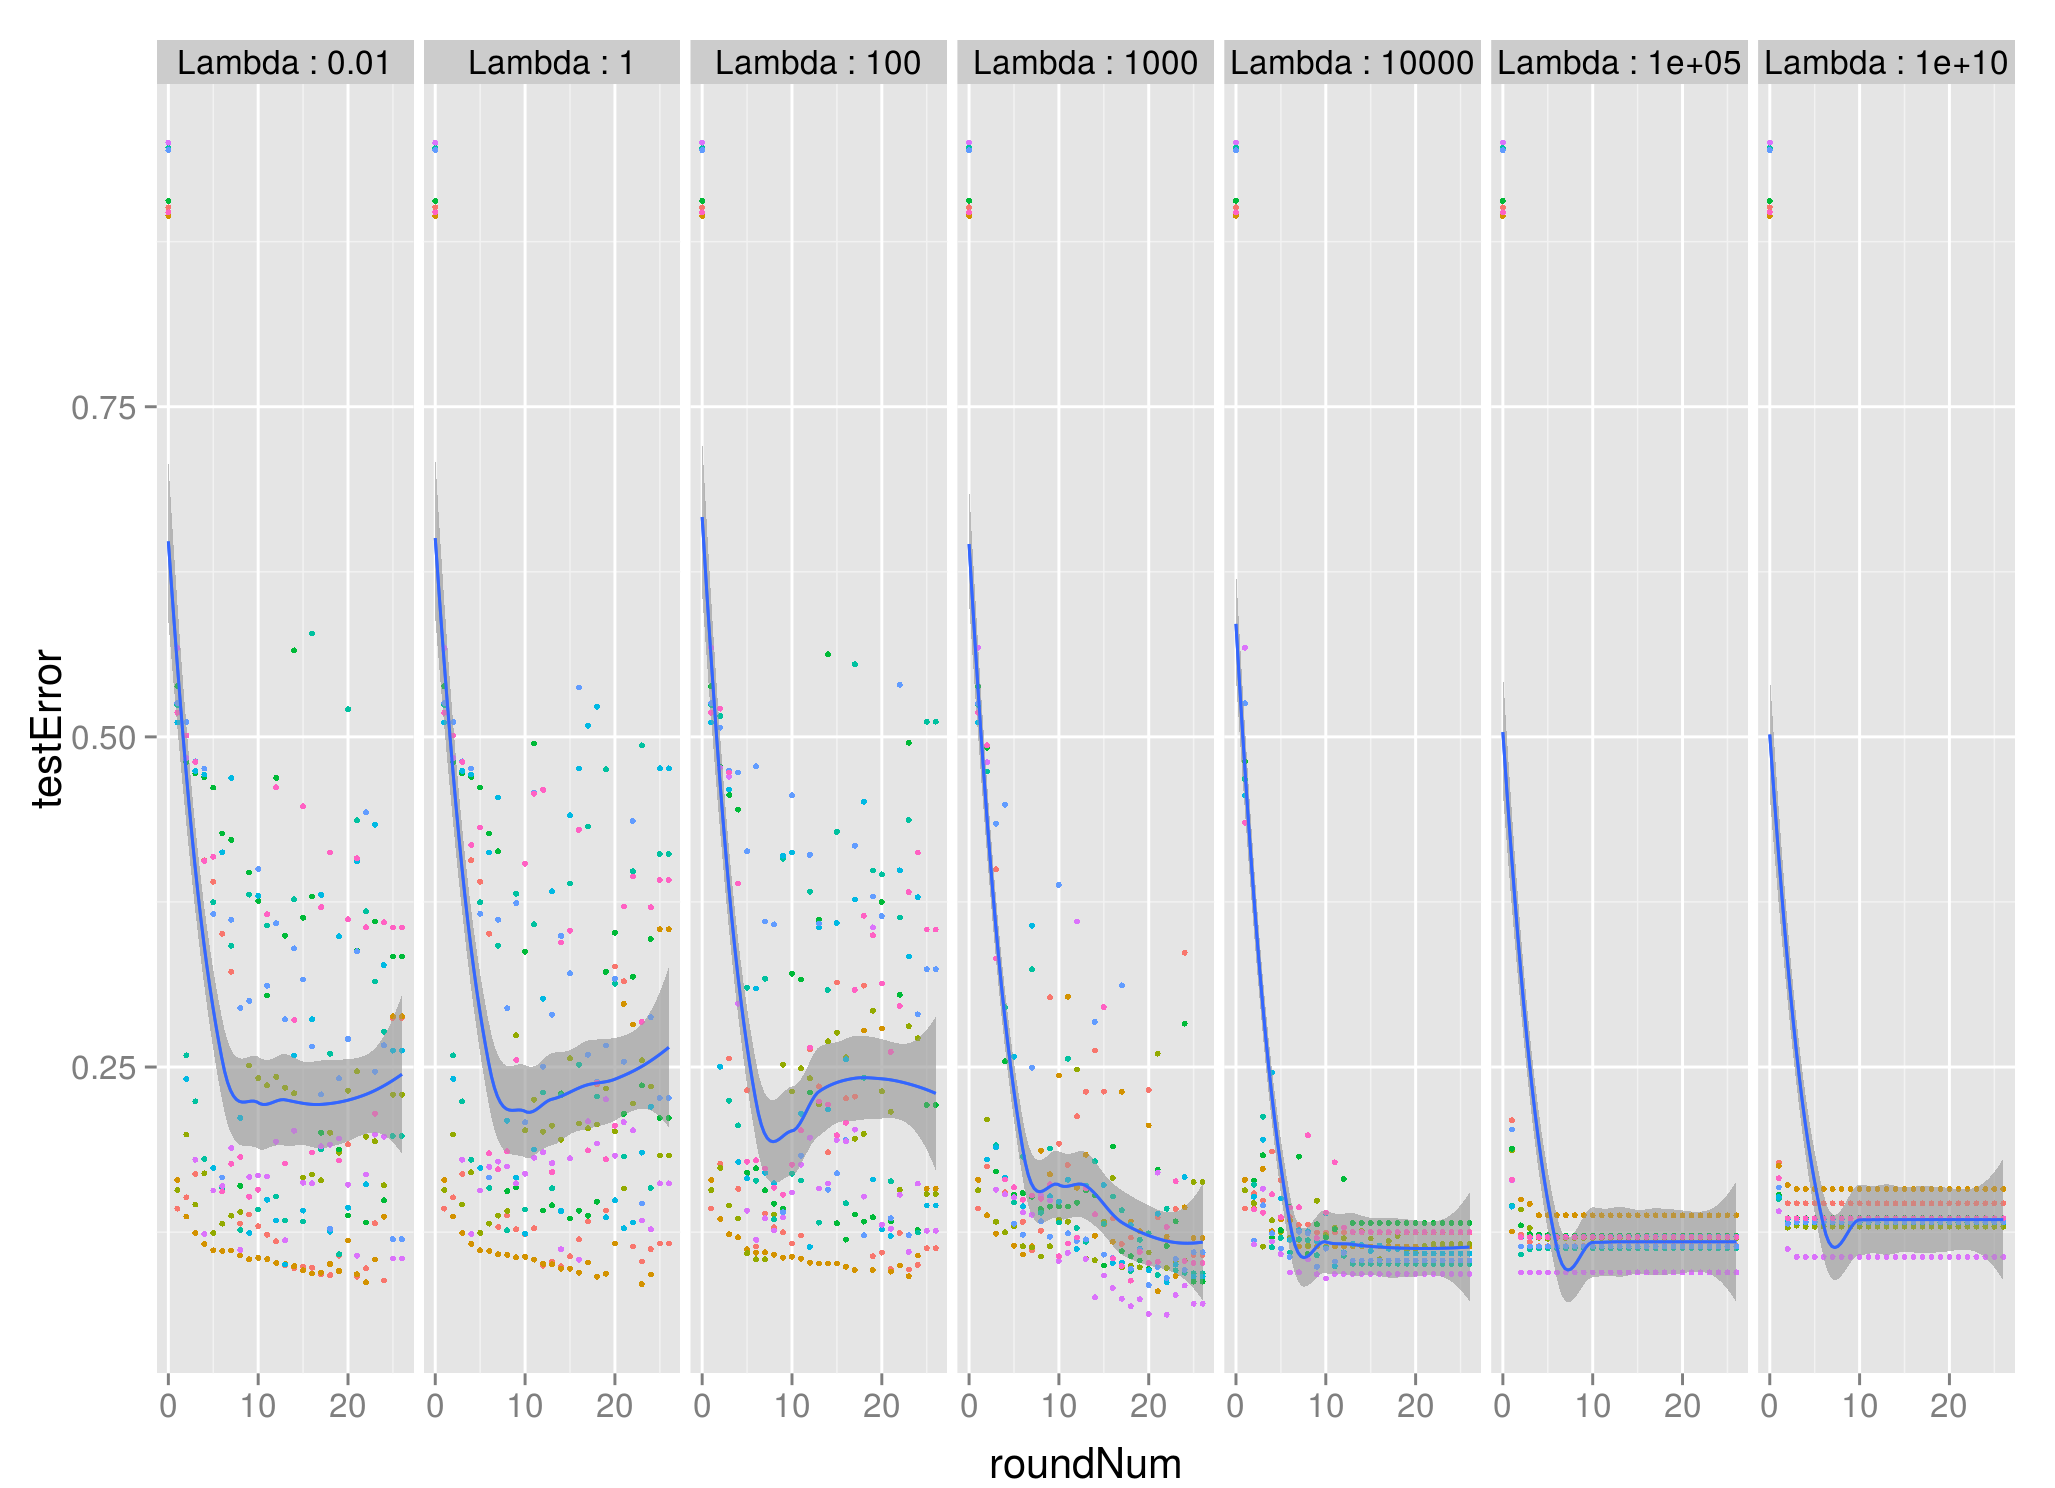
\includegraphics[width=1.0\textwidth]{images/testLoss_nuclei_equalScale.png}
  \caption{  Looking at the curve of Test Error over time with different lambdas we can see that higher lambdas converge faster and if one sets lambda two low it does not seem to converge at all. Data( Single Channel 3D Nuclei \cite{ucsbData})} 
  \label{fig:lambdaTestNucl2}
\end{figure}


\section{Data Dependent Pairwise models}
To examine farther why the data dependent models did not outperform the standard pairwise model we plot the convergence rate of the pairwise indexes of $w$. As seen in Figure \ref{fig:mitochonPairwiseNorm} the curve of the norm of $w_{pairwise}$ over sequential rounds is much steeper for the standard pairwise model as compared to the two data dependent models presented. This indicates that the data-dependent pairwise terms may have needed more rounds to converge than simple pairwise model. A rational for the difference in convergence rate could be that the data dependent term can only gain information from the portion of the transitions which are binned into that group of the data dependent pairwise model hence it probabilistically requires more data to gain the same amount of information in each bin. To test this hypothesis we reran this experiment with larger suboptimal lambda selections. In Figure \ref{fig:mitochonDifLambdaShLoss} we see the Structured Hingle Loss over time and as the lambda gets higher there is a trend of the data dependent models improving their gain over the simple pairwise model. indicating that the data dependent pariwse term could converge better with a higher lambda value but such high lambdas result in lower Test Error due to the unary term as described above. Preliminary results with high number of rounds $\geq 110$ show the data dependent models starting to converge and improving the test error over simple pairwise models. Put since the unary term does not require this many rounds to converge we purpose an addition to the current system which would allow for different regularization of the pairwise term seperatly from the unary term. 




\begin{figure}
  \centering
  \figuretitle{ Pairwise W norm over Sequential Rounds}
  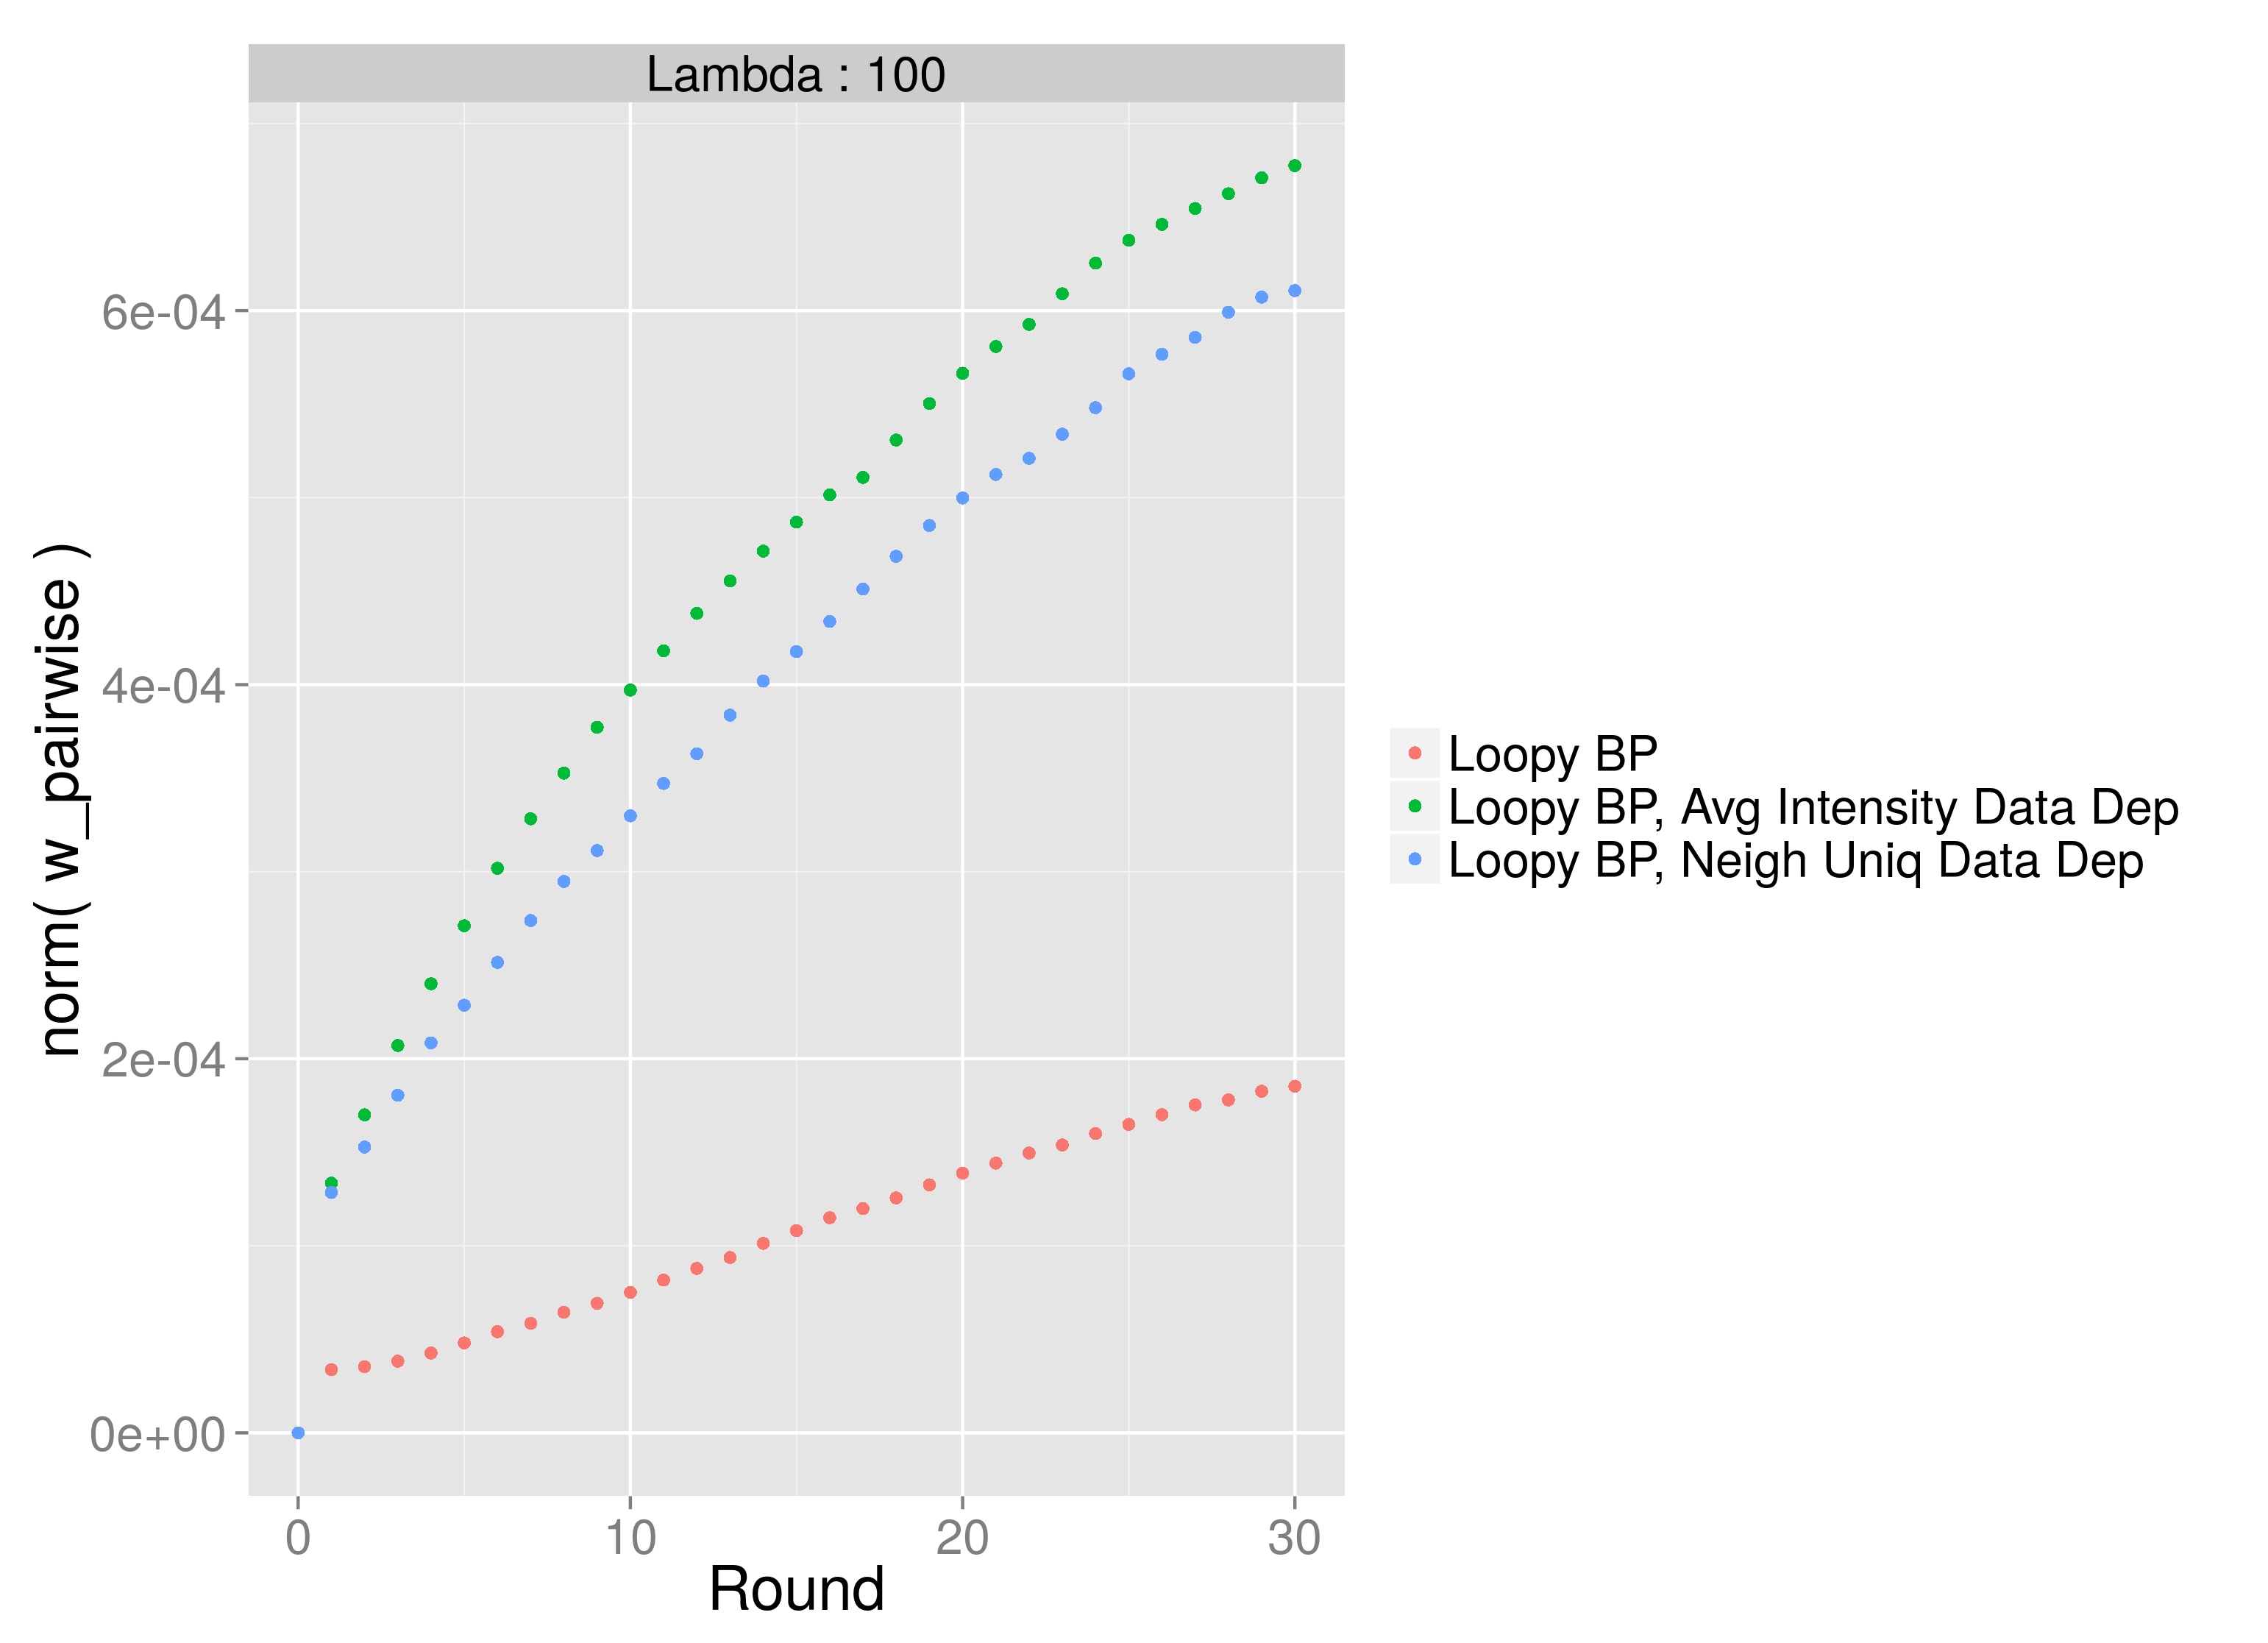
\includegraphics[width=0.8\textwidth]{images/mitochonSplit_pairwiseWnorm_overTime.png}
  \caption{ The above graph displays the norm of the pairwise portion of the weight vector. The weight vector is always initialized to zero at round zero. The curve of the norm of $w$ can indicate convergence behavior. In this experiment it appears that Loopy BP (the Simple Pairwise model) is converging faster than both data dependent pairwise models. Data:( EM Mitochondira Labeling split into $82^3$ cubes with super-pixels of size $S=10$ \cite{mitochondriaData} )} 
  \label{fig:mitochonPairwiseNorm}
\end{figure}

\begin{figure}
  \centering
  \figuretitle{ Structured Hinge Loss over Time, including Linear Trend Line }
  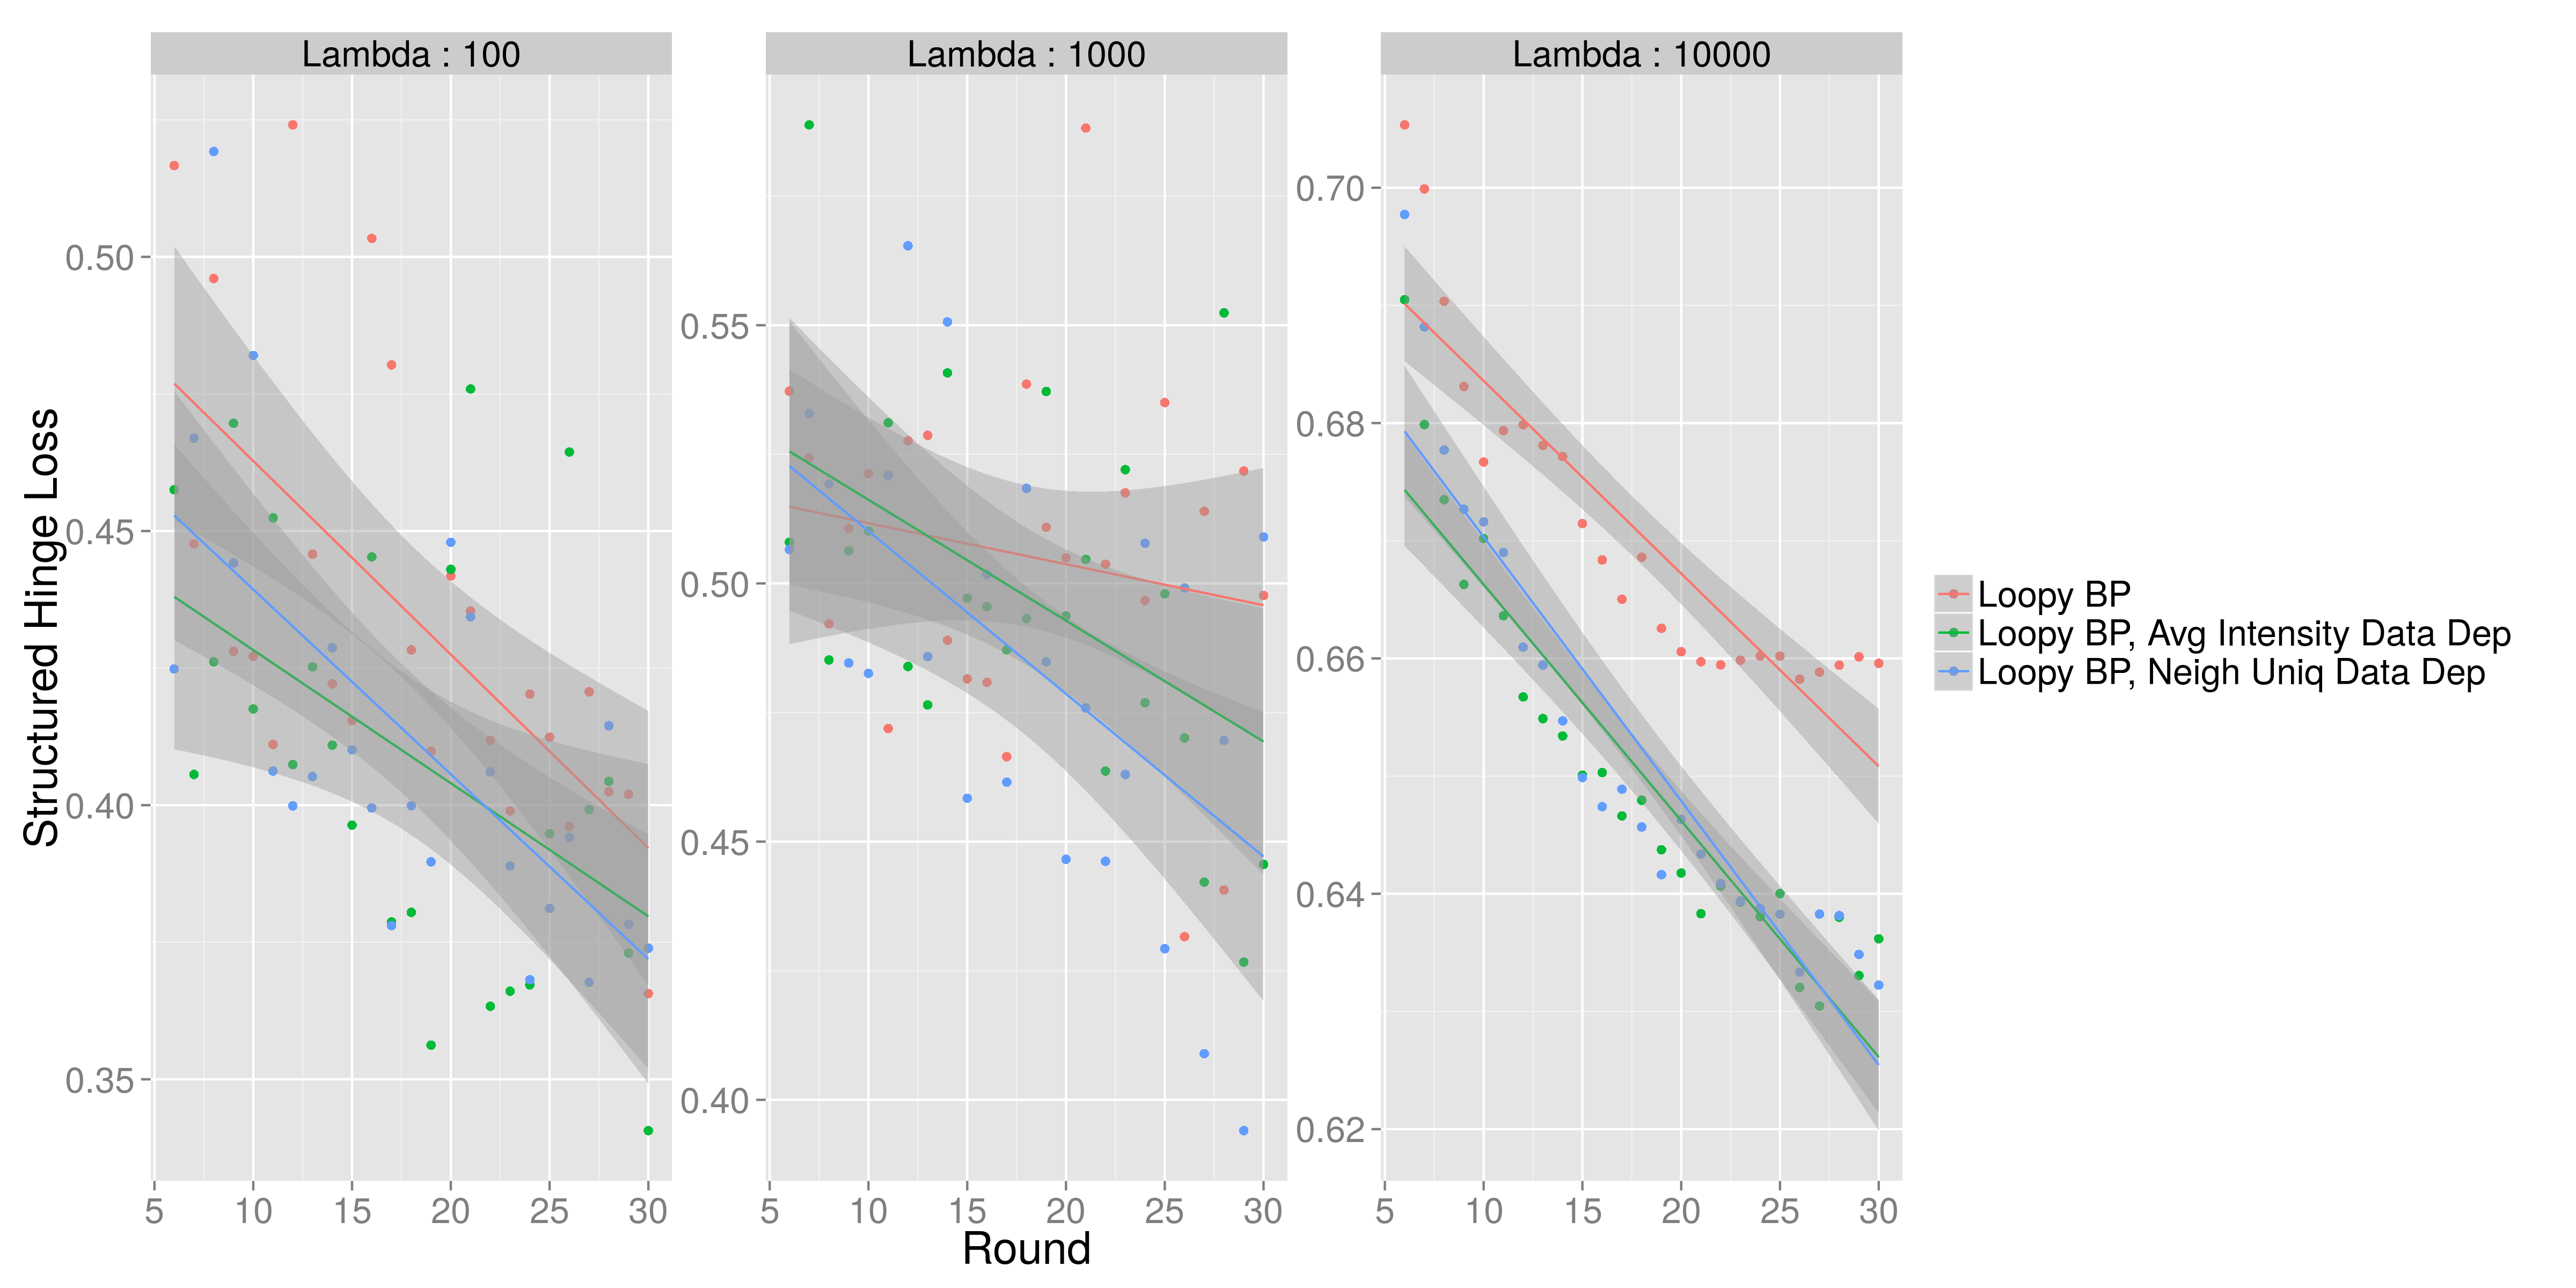
\includegraphics[width=0.8\textwidth]{images/mitochonSplit_shloss_difLambda.png}
  \caption{  This Figure displays the Structured Hinge Loss ($\shlossexp$) over time of the different pairwise models. With the added linear regression line we can see that as we increase Lambda the difference between the simple pairwise model to the data dependent models increases. Higher lambdas cause faster convergence hence we conclude that data dependent models require more rounds to converge. Data:( EM Mitochondira Labeling split into $82^3$ cubes with super-pixels of size $S=10$ \cite{mitochondriaData} )} 
  \label{fig:mitochonDifLambdaShLoss}
\end{figure}




%%%%%%%%%%%
%
%
%
%
%
%
%
%
%
%
%
%
%
%
%
%
%
%
%
%%%%%%%%%%%





\chapter{Distributing Workload}
The dissolve framework which we used to solve the SSVM was written with distribution in mind by 

\section{Single Node, Multiple cores}
Spark can be used to distribute the inference work over a cluster but also it utlizes local parallelization without writing multi-threaded code. In some computing environments it may be cheaper to use one 36-core machine versus nine 4-core machines, or it could be advantageous for the user to avoid time lost in network synchronization.  When distributing on one machine one must consider memory limitations, by default spark assigns 512mb per driver hence if one is running a 36-core machine other than the ram needed for the driver it must have 18432mb available for all the executors. When using \codeInLine{sbt run-main ch.ethz.dalab.dissolve.examples.neighbourhood.runReadTrainPredict } to start the local job one can specify the internal driver memory used with the \inputArgs{spark\_driver\_memory} which should be specified as a string just as in the spark config. 
\par
As is typical when distributing we do not get perfect scaling as adding more executors requires more synchronization work. Figure \ref{fig:singelNodeScale} shows total training time required for the MSRC dataset on a 8 core machine varying the number of local-spark-executors. 
Even when setting the number of executors equal to the total number of cores available we did not observe any thrashing but rather still saw a slight improvement from 7 to 8. Scalling well even up to the max number of cores can be partially attributed to the design where the driver has little work until a round ends and the executor results needto be combined, during this time when the driver is active the executors are ideling. Hence they do not compete for computational resources even when both are on a single machine. The increase in the time needed for the Spark Driver to coordinate the different spark-executors is visualized by the difference between blue and green points (Total Training Time - Theoretically perfect Scaling). From one to two exectuors there is a jump in this difference because this is when merging of results first occurs. As the number of executors increases the distribution coordination time increases but with negative second derivative. Additionally we plotted what training time we would expect if the entire system only needed to run the oracleFn and was being distributed perfectly in Red (Decoding Time / number executors). As expected this curve is slightly above the perfect theoretical scaling because of course the cores of the CPU and the work we do inside the oracleFn are not completely independent. To farter ensure that the oracleFn is being scaled aswell as we think we reran the above experiment with significantly higher loopy belief propagation iterations such that the individual oracle calls are significantly longer. In Figure \ref{fig:singelNodeScaleLonger} we see that under these conditions we get scaling which is even closer to theoretically perfect hence affirming that the oracle calls themselves are very well distributed. 



\begin{figure}
  \centering
  \figuretitle{ Single Node Scalability by Varying Executors  }
  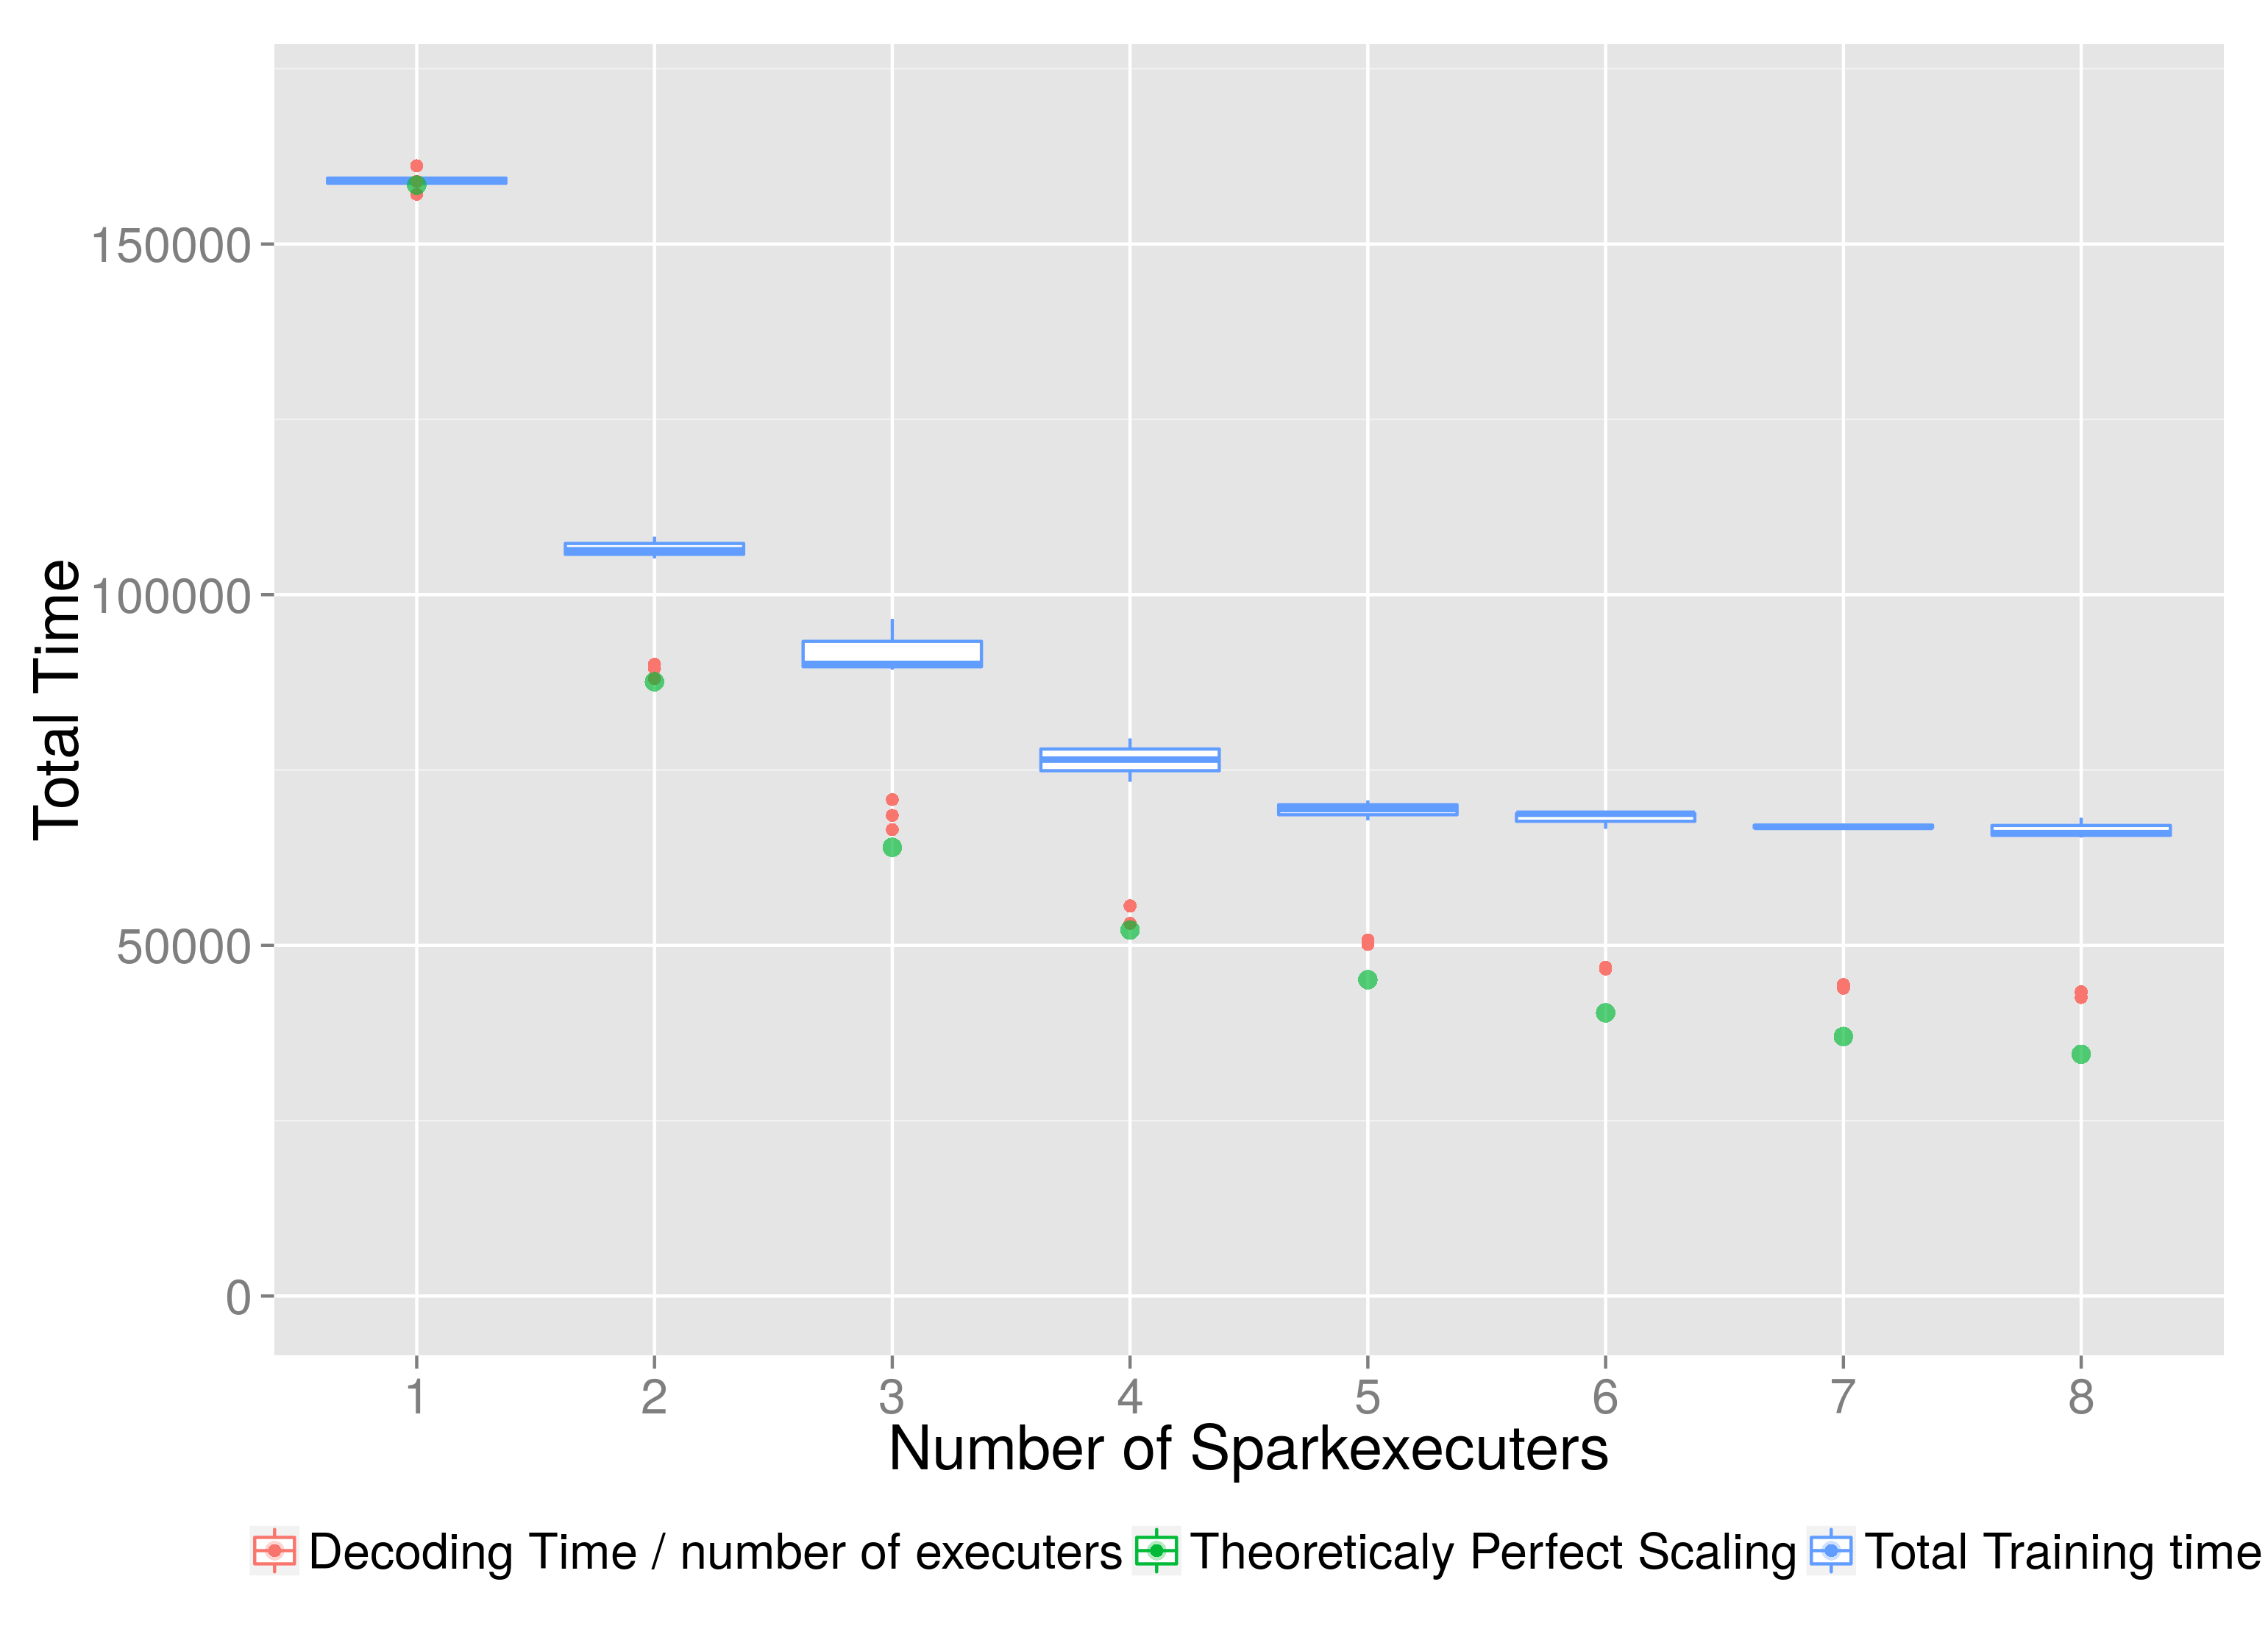
\includegraphics[width=1.0\textwidth]{images/singleMachineScalability.png}
  \caption{ In blue we see the total time to train the model as measured on the driver node, this time consists mostly of time spent in the oracleFn but also there is a constant overhead of ~16000ms and for the experiments with greater than one executor we have a significant amount of work dont on a single thread when combining and coordinating the executors. The red points are the recorded total amount of time spent inside the oracleFn divided by the number of cores available to spark shifted to match the constant overhead of the single executor experiment. The Green points are the theoretically best scaling extrapolating from the pure decoding time of the experiment with only one executor by simply dividing by the number of cores and also shifting the constant overhead.  } 
  \label{fig:singelNodeScale}
\end{figure}
\par 

\begin{figure}
  \centering
  \figuretitle{ Single Node Scalability by Varying Executors (More decoding iterations) }
  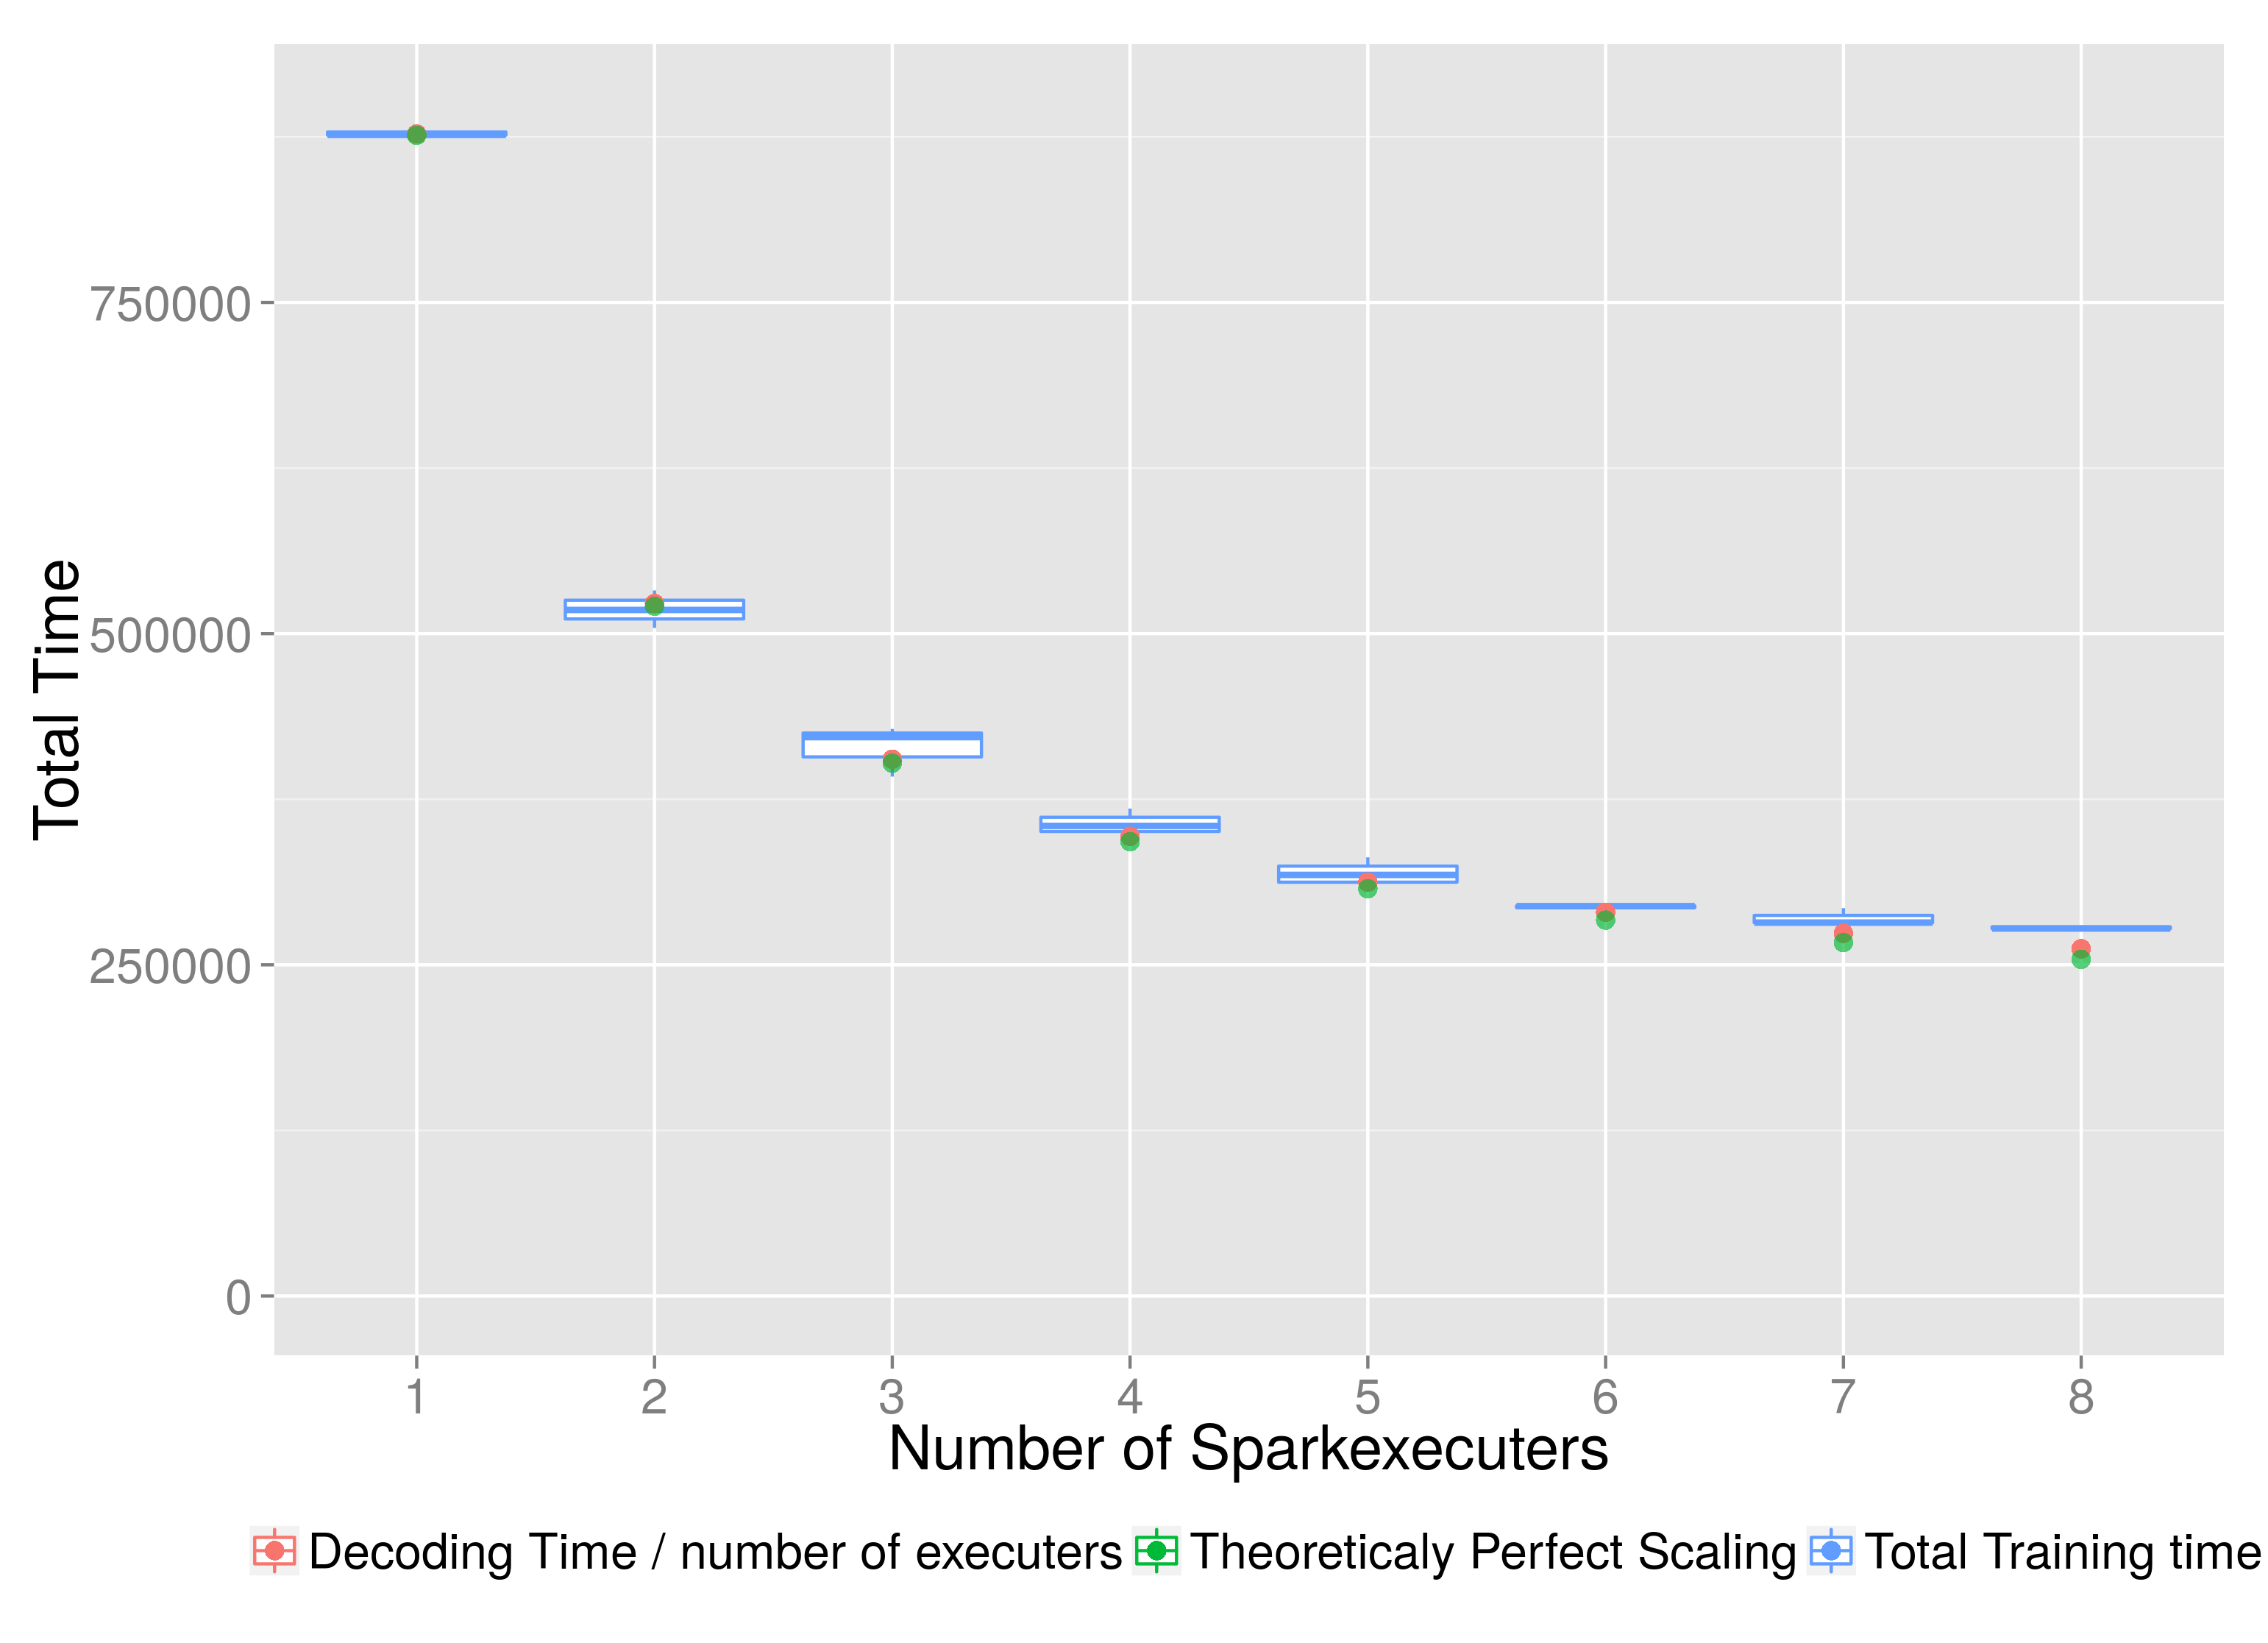
\includegraphics[width=1.0\textwidth]{images/singleMachineScalability_longerDecoding.png}
  \caption{ See description for Figure \ref{fig:singelNodeScale} we reran the same experiment but with more loopy belief iterations to get a more precise max oracle decoding. Comparing to Figure  \ref{fig:singelNodeScale} we see an even better scaling with very little increase in context switching time as seen by the difference to the perfect scaling curve in green. This was expected as we modulated on parameter which only effects the max-oracle timing. } 
  \label{fig:singelNodeScaleLonger}
\end{figure}
\par 

\section{Multiple Nodes, Single core}
As we expected on tasks with a high max-oracle decoding time the additional time required for spark to recombine results over the network does not significantly impact scalability when contrasting to parallelizing on a single machine without network time, see Figure \ref{fig:scaleDistrmsrc1} for details. Additionally the data that needs to be transferred over the network is very minimal because of how dissolve-struct is designed. Dissolve-struct when configure to run Distributed-BCFW utilizes a method optimized for low network traffic called CoCoA (Communication-efficient distributed dual Coordinate Ascent) \cite{cocoa}.CoCoA can be applied to a large class of linear regularized loss minimization objectives, which includes the SSVM image segmentation objective \ref{optimizationFunc}. The primal-dual structure of these problems was used to aggregate partial results from local computations in such a manner that reduced network traffic and avoided conflicts with updates made by different machines. It has also been shown that the CoCoA communication and weight update scheme has little effect on the total amount of computation needed to achieve the same accuracy  as globally communicating methods \cite{cocoa}. 


\begin{figure}
  \centering
  \figuretitle{ Cluster Scalability, Single Core per Machine }
  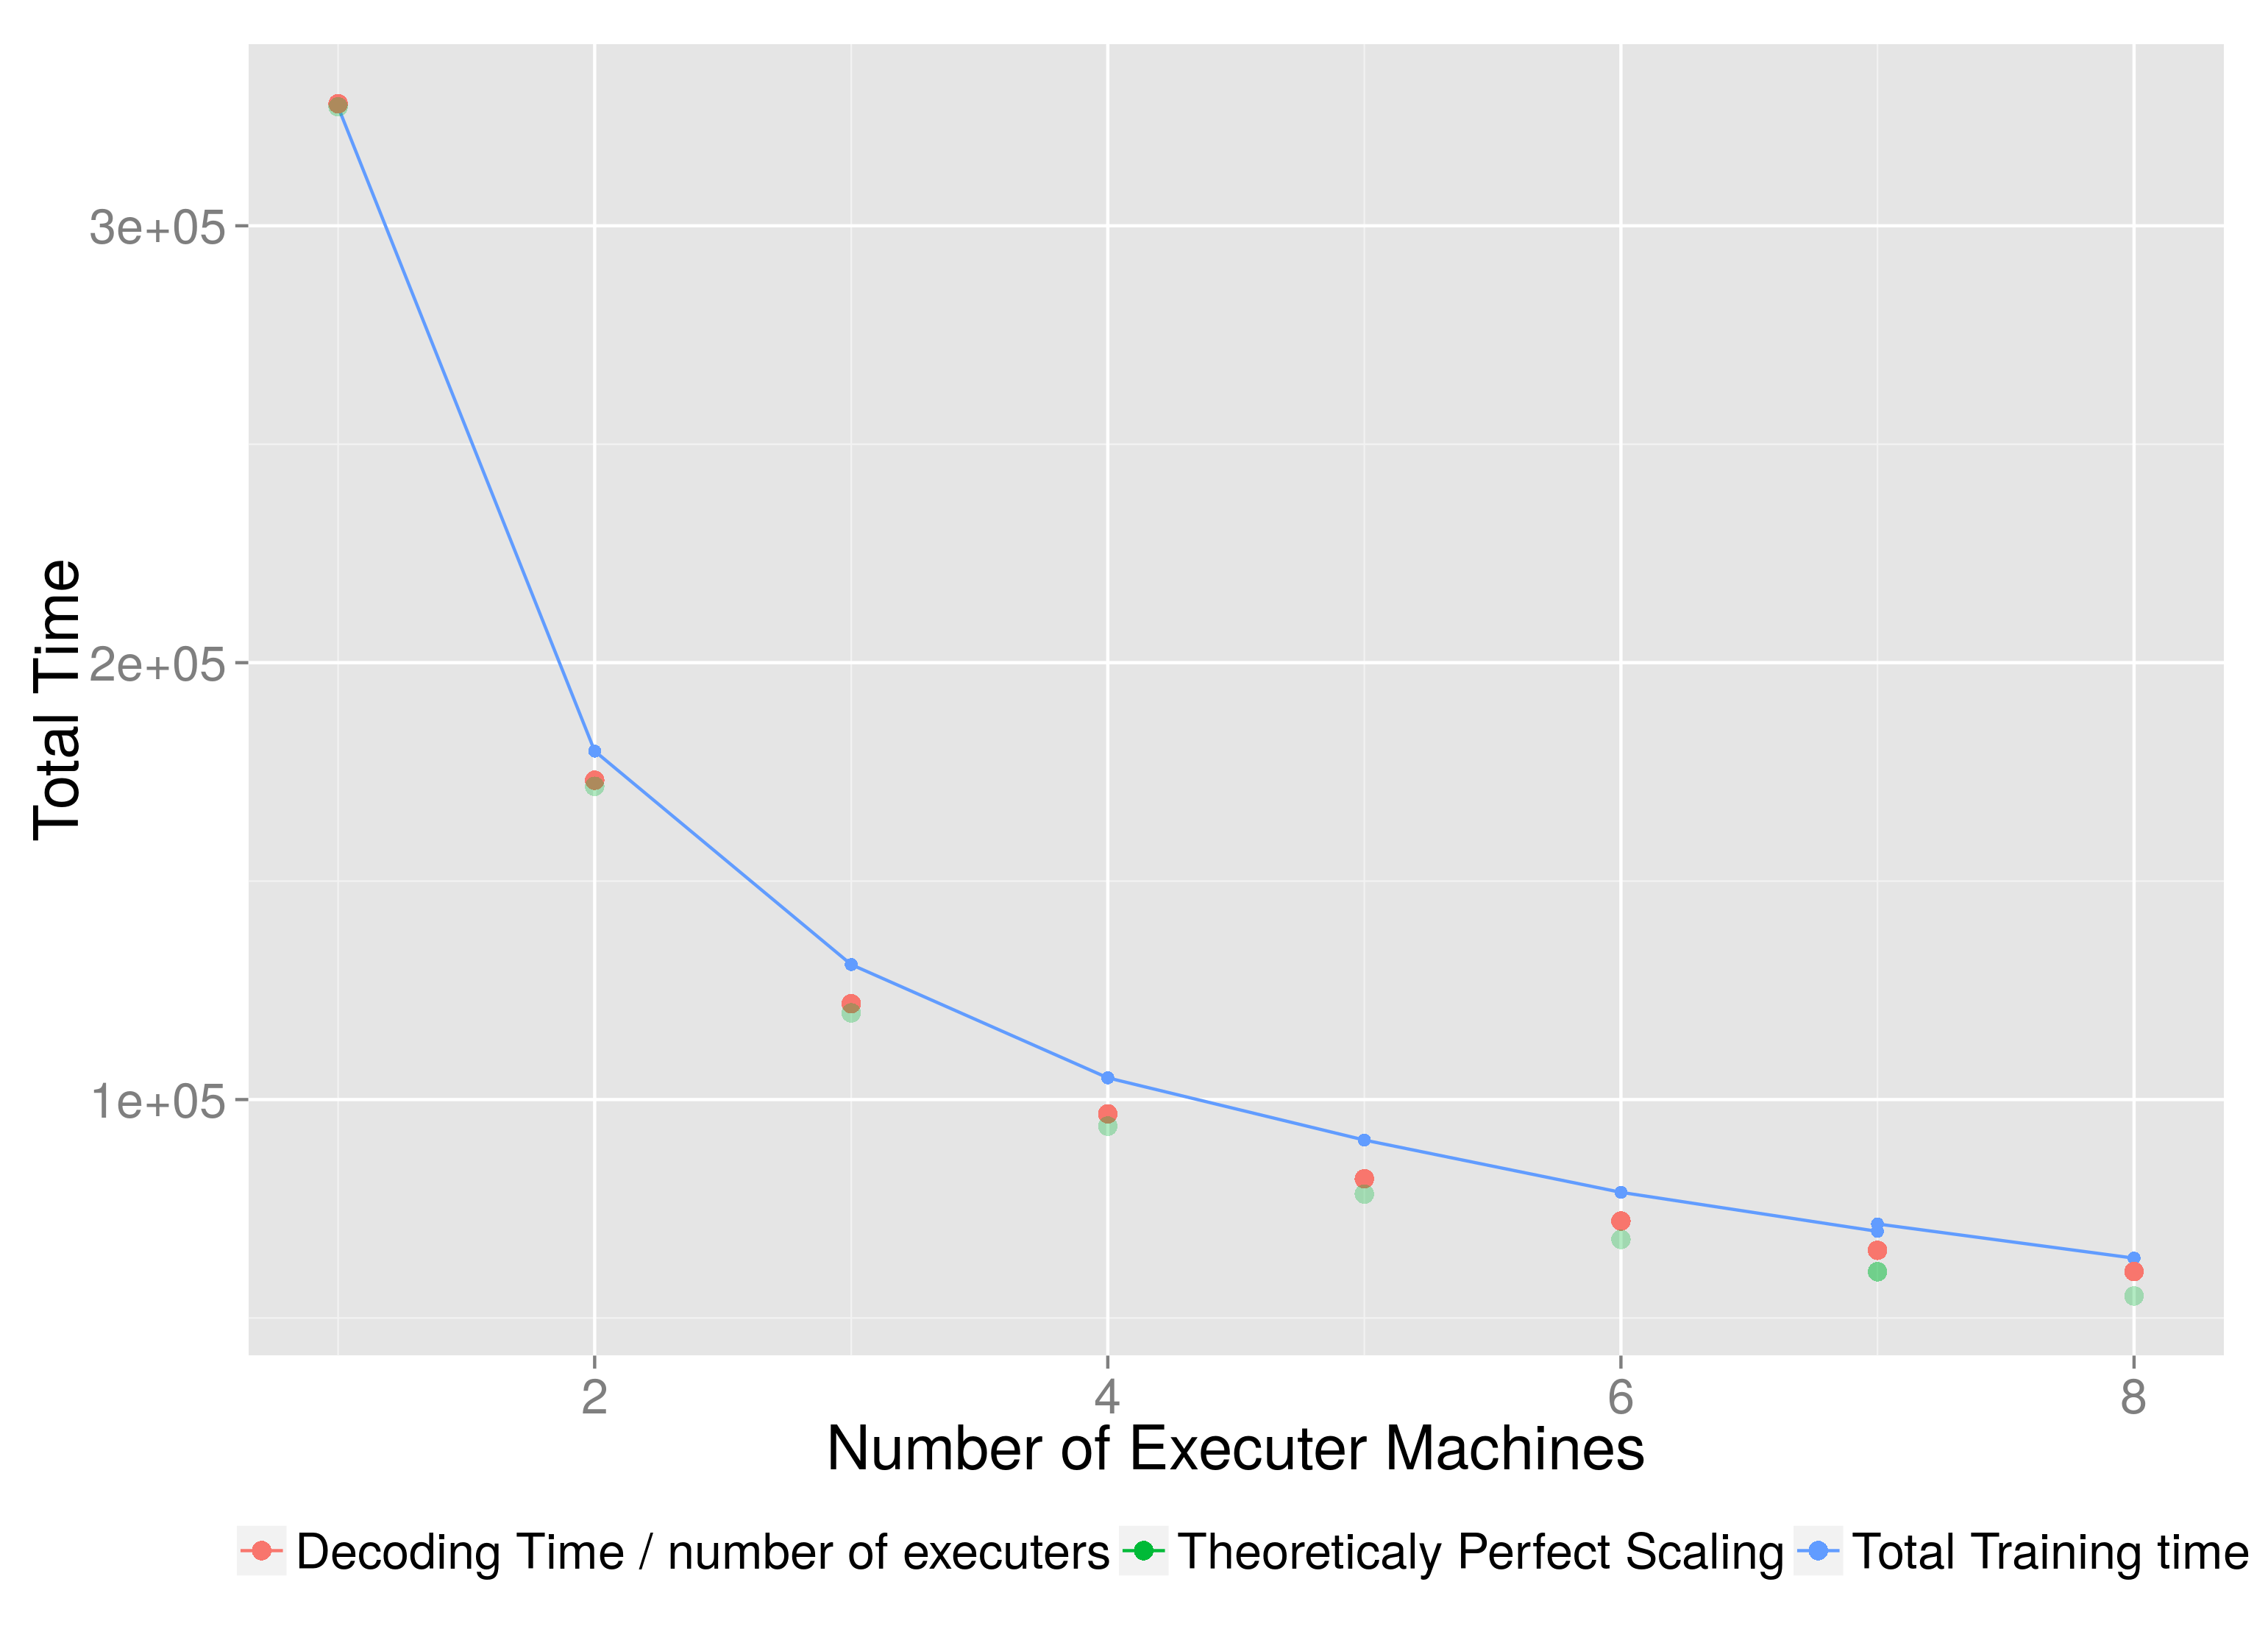
\includegraphics[width=1.0\textwidth]{images/scalabilityDistributed_msrc.png}
  \caption{ This Figure displays the total training time required for the entire MSRC data set on a varying number of m3.large AWS virtual machines each configured to use just one core. We can again see a good scaling curve as the true train time is close to the expected train time if there was no delay in context switching (Theoretically Perfect Scaling). Bu the scaling is not perfect and as more machines are added the difference in training time produced by additional time used on the driver node for recombination and coordination increases the distance to perfect scaling. } 
  \label{fig:scaleDistrmsrc1}
 
\end{figure}


\chapter{Discussion}
While the EM Mitochondria dataset resulted in good performance of the pairwise model there were others like the MSRC dataset where the unary model was not significantly overtaken. As explained in the results section \ref{smoothness} we find that the pairwise models do produce much smoother (and therefore more natural) predictions. But this is not captured in the Hamming distance loss function and hence on some datasets the unary gets higher accuracy even if the prediction has single labels in a neighbourhood which we know a-priori would be impossible. We suggest for future work to develop a new loss function which evaluates the accuracy on the test set by also capturing the natural plausibility of the output produced. In many applications it is more important for the segmentations to be biologically plausible than having the highest per pixel match to the ground truth \todo{citation needed}. Some replacements to the Hamming distance have been purposed. The PASCAL natural image segmentation challenge was measured using the per class Jaccard distance \cite{everingham2010pascal}. A measure which encourages labelling with the correct size was pruposed by Pletscher and Kohli \cite{pletscher2012learning}. Balancing false positives versus false negatives with class priors was attempted by Lempitsky et. al. \cite{lempitsky2011pylon}. But all the above loss functions do not consider the topology of the labelled objects as a whole.
\par
Still with the simple weighted loss function used for all our training we achieve satisfying results with very good scalability and preliminary research has shown that the accuracy can be vastly improved by using more sophisticated features. 


\section{Expansion of Features}
We did not focus too much attention on the features as their choice is very dependent on the data at hand. Still for biological data we would like to expand the set of pre-installed features to include Ray projection features \ref{smith2009fast}. And recently deeplearning features have found a lot of success on natural image segmentation problems \cite{krizhevsky2012imagenet}. These Deep Learning features actually result in a much higher dimensional problem than what we are solving but since we solve it in the dual and representing alpha as sum of spares vectors the system is robust to the feature vector becoming very large. 
\section{Expansion of ScalaSLIC}
We chose to perform the preprocessing on single machine because it only needs to be done once before training and in order to keep this package simple as it will be published open-source separately. But in practice we found that the preprocessing takes a significant amount of time and could easily be distributed on a per image basis. Once this preprocessing step is distributed one could also expand the distance measure to include more complex features than just the LAB space distance. 
\section{Expansion of the SSVM}
One clear improvement we would have liked to test would be to transform the dual problem into a kernel space because it would allow us to find a non linear decision boundary. While it is clearly advantageous from a learning theory perspective it would come at additional computational complexity because to get $\weightVect$ for synchronization between nodes one would have to sum up all the support vectors chosen thus far. But it is worth attempting empirically because bringing the features into a space where classes are easily separable will make the max-oracle problem easier and hence one could possibly reduce the number of iterations used for LoopyBP or Mean Field. 
\section{Improving Automation}
As we described in section \ref{sec:Lambda} the lambda parameter is critical for good convergence of BCFW. The user is advises to always rerun their experiment with lambda constants at several scales to find the best range. Lambda could easily be selected automatically by minimizing the cross validation error on the training set. Additionally we explain the relevance of compactness parameter $M$ for the super-pixel preprocessing described in section \ref{slicParams}. The parameter $M$ is independent of the choice of lambda and could be optimized by running slick several times and optimizing for the most uniformity of ground truth labels within each super-pixel. 


\appendix

%
%
%
%
%
%
%
\chapter{Implementation Details }
\section{Preparing and Reading in data}
When using our provided data importing functions we expect the data to be stored in two folders one for the raw image files and one folder for the ground truth mask. These folders must be labled "Images" and "GroundTruth" respectively. Both raw images and ground truth can be in .bmp, .tif or .png formats but the format has to be uniform throughout a dataset. Additionally it should be noted that the ground truth mask is mapped to its image only by file name so in the end the images folder and the groundtruth folder must have the same number of files with the same set of names. Ground truth masks labels are read in per pixel color or grayscale value, the ground-truth mask should be considered a space indexed label mapping so each label must have exactly one value here, which also means these files should be much smaller than the image files. The data location is specified by the input argument "dataDir=".
\subsection{Caching}
If the user chooses to run our preprocessing functions for creating super-pixels, extracting features and constructing the graph, then all of these will be cached on disk in the same folders where the data resides. The caches are performed for each image individually and are named after the raw image of origin as well as some information about what options where used when creating this cache. With this very simple caching system we prevent the user from having to recompute every image in the event of a crash, or when changing a few parameters for later portion of the pipeline. If the user wishes to rewrite the cache without checking if there are matching flags in the files one should specify the input argument "recompFeat=true" or the user can change the "runName=" input argument as it will a new set of caches while leaving the old ones as is. The files ending in ".mask" in the Images folder contain the mapping between pixel index to super-pixel id. Files ending in ".graph2" contain the completed graph structure of the associated image, I.E. nodes which only save their own features and the node id's of their neighbors. Files ending in ".classCount" , ".colorlabelmapping2" and ".transProb" contain the class frequency count, map between colors used in the groundtruth files and internal label id and the transition probabilities between labels respectively. The files ending in ".labels2" contain the cache for the true labelled graph of these training dataset. 


\subsection{Feature Standardization}
Standardizing features is important especially when some features are degrees of magnitude larger than others, for example when including \inputArgs{featAddIntensityVariance} and \inputArgs{featHistSize}. 




\section{Features}
Since our data is split up into non uniformly shaped super-pixels we could not use off the shelf feature functions. We implemented some basic features like color or intensity histograms, Co-occurance matrix, and some features based on the super-pixel graph structure like the sum of neighbor histograms, in neighbourhood intensity uniqueness and some others. All these features are computed after the super-pixel bounds have been determined. Most of the features are extracted by once running overall pixels in the image and adding to some moving average of the feature indexed by the super-pixel id of that corresponding pixel. If using our graph construction script \codeInLine{genGraphFromImages()} the features are specified as arguments into either \codeInLine{featureFn} or \codeInLine{afterFeatreFn}. As the name implies afterFeatureFn is run after the graph is constructed and provides the feature functions with the graph edge information, featureFn is for unary features only. If also using our start-up main \codeInLine{ch.ethz.dalab.dissolve.examples.neighbourhood.runReadTrainPredict} then the feature functions are constructed for the user who only has to specify which features are desired. 
\subsection{Predefined Feature List}
All below features can be specified in the runtime arguments of \codeInLine{runReadTrainPredict} for color, greyscale , 2d and 3d image datasets. 

\begin{description}
\item[\inputArgs{featIncludeMeanIntensity}] Averages all pixels assigned to a super-pixel into one mean intensity. For color this mean intensity is the corresponding converted greyscale intensity. This feature may also be added to the metadata of a node such that the datadependent pairwise models can use it.  
\item[\inputArgs{featHistSize}] If set above Zero we construct a normalized histogram of colors or gray scale intensities with equally sized bins. Bin sizes are always $\frac{255}{featHistSize}$. The color version of this histogram constructs bins per color dimension and but keeps the same number of bins specified, hence for color \inputArgs{featHistSize} must be divisible by three.
\item[\inputArgs{featUseStdHist}] Will construct non histigrams with non uniform bin sizes. Rather it initially computes a global distribution of intensities and constructs bins which should contain approximately equal datapoints. \inputArgs{featHistSize} is still used to specify the number of bins but only the standardized bins are used in the features. The bin sizes are computed once for the whole dataset and are ofcourse not adjusted for new data hence the training set must be sufficiently large for the distribution to be accurate. 
\item[\inputArgs{featCoOcurNumBins}] Co-occurance matrices are constructed again binning all pixels into uniformly sized ranges of the intensity spectrum and then counting all occurrences of a pixel binned to bin $A$ neighbouring a pixel in bin $B$. Again the number of bins must be divisible by three if used on color data. One can specify exactly which kind of neighborhood should be used by default we only consider one pixel hop and no diagonals, to change this one must alter the feature function call with different $directions$ input. 
\item[\inputArgs{featAddOffsetColumn}] This will simply add a column of ones into the feature vector giving the SSVM one more degree of freedom for its decision boundary. 
\item[\inputArgs{featAddIntensityVariance}] calculates pixel intensity variance per super-pixel, for color images this is again the converted greyscale value $\frac{Red}{3}+\frac{Green}{3}+\frac{Blue}{3}$. 
\item[\inputArgs{featUniqueIntensity}] Computes mean intensities and variances if not yet computed for all super-pixels then measures the number of standard deviations away from the mean of a super-pixels one hope neighbourhood its own intensity is. 
\item[\inputArgs{featUnique2Hop}] Same as \inputArgs{featUniqueIntensity} but using a 2 edge hope neighbourhood. 
\item[\inputArgs{featNeighHist}] Computes histograms per super-pixels as in \inputArgs{featHistSize} and then sums all the histograms of neighboring super-pixels not include the data from the super-pixels own space and then normalizes. \inputArgs{featHistSize} again determines the size of the bins used here. 
\item[\inputArgs{featAddSupSize}] The count of the number of voxels assigned to a particular super-pixel. 

\end{description}



\section{Additional Runtime Arguments }

Critical 
\begin{description}
\item[\inputArgs{useNaiveUnaryMax}] Setting this to true will result in dissolve using the simple per node max decoding inside the oracle function. See section \ref{sec:unaryMax}.
\item[\inputArgs{useMF}] If Set to true, dissolve will use the Mean Field appoximation to solve the max oracle problem. See Section \ref{sec:meanField}
\item[\inputArgs{modelPairwiseDataDependent}] If set to true, the max oracle will be performed on a CRF where the pairwise potentials are dependent on the label but also a function of the two super-pixels features. This model was only implemented for Loopy Beliefe Propagation decoding.  See Section \ref{sec:dataDep}
\item[\inputArgs{mfTemp}] Specify any Double value for use as the Temperature paramater in the Mean Field decoding. See Section \ref{sec:meanField}
\item[\inputArgs{useLoopyBP}] If set to true, Loopy Belief Propagation will be used for the max-oracle function. See \ref{eq:loopybp
\item[\inputArgs{loopyBPmaxIter}] Loopy Belief propagation iterations before returning the max-oracle decoding. Training time scales linearly with the number of iterations. 
\item[\inputArgs{useRandomDecoding}] For debugging and comparison purposes we have included a max-oracle which returns a random $\yVect$. 
\item[\inputArgs{roundLimit}]


\item[\inputArgs{onlyUnary}] Used to specify if the max oracle should run decoding on a CRF with only unary potentials, see Section \ref{sec:crfvarations}
\item[\inputArgs{lambda}] The regularizing parameter see section  \ref{sec:Lambda}
\item[\inputArgs{doLineSearch}] 
\item[\inputArgs{numClasses}] The expected range of labels.
\item[\inputArgs{isColor}] Set to true if the data being read in is using RGB leave false if data is grey scale. 
\item[\inputArgs{useClassFreqWeighting}] If set to true the lossFn will not be a zero-one loss but rather every missclassificaiton is counted as one inverse class frequency.  This is import to set as true if using dataset which has large imbalance in the label counts. 
\item[\inputArgs{superpixelSize}] Set to an Integer greater than zero this is the $S$ parameter in our SLIC implementation. See Section \ref{sec:slicAlgo}
\item[\inputArgs{slicCompactness}]  Set a double value greater than zero, this corresponds to the $M$ paramater in SLIC. See Section \ref{sec:slicParams}
\item[inputArgs{dataFilesDir}] The path to your training raw images and ground truth. In this folder we expect a subfolder named GroundTruth and one named Images. The user can also specify these seperatly with \inputArgs{imageDataFilesDir} and \inputArgs{groundTruthDataFilesDir}
\item[\inputArgs{numberOfCoresToUse}]


\end{description}

\section{Example Run}

\todo{put code for some example runs and file structures}
For viewing the predicted labels we recommend UCSB's bioView3D \cite{bio3dViewer}. 

Optional
\begin{description}
\item[\inputArgs{trainTestEqual}] If set to true, the preprocessor will not reserve any data for testing but rather train on all possible data. 
\item[\inputArgs{squareSLICoption}] If set to true, the SLIC preprocessing will simply produce square super-pixels. Run time for these super-pixels is only $\mathcal{O}(n)$. 
\item[\inputArgs{LOSS\_AUGMENTATION\_OVERRIDE }]If set to true optimization the objective without considering loss between graph labels. As in $\min_{\weightVec} \frac{\lambda}{2} ||\weightVec||^2 \frac{1}{n} \sum_{i=1}^n \max_{y in \ySpace} \langle \weightVec , \jointFeatureMap \rangle$
\item[\inputArgs{initWithEmpiricalTransProb}] Will precalculate the class transition probability table and initialize the pairwise section of the $w$ to these values. 
\item[\inputArgs{dbcfwSeed}] A random seed used inside BCFW setting this to non -1 value will allow for deterministic output. 
\item[\inputArgs{runName}] A simple string used in logging and in the cache files.
\item[\inputArgs{checkpointFreq}] 
\item[\inputArgs{dataGenSparsity}] The desired percentage of the ground truth which is background when generating synthetic data. See section \ref{sec:synthDataGen}
\item[\inputArgs{dataNoiseOnlyTest}] If set to true the data generated will only add the specified noise to the test set not the training dataset. 


\item[\inputArgs{dataGenCanvasSize}] Number of pixel rows/columns per image being generated. Images are always square. 
\item[\inputArgs{dataRandSeed}] A seed value for the random number generators used in the data synthesis functions. If set to a non -1 value then the data generation is deterministic.  Allowing experiments to be run over different machines without having to transfer the data. 
\item[\inputArgs{dataGenSquareSize}] The size of the super-squares used in synthetic data generation, see Section \ref{sec:synthDataGen}
\item[\inputArgs{dataGenSquareNoise}] A decimal between 0.0 and 1.0 specifying how much SuperSquareShift noise should be added, see Section \ref{sec:synthDataGen}
\item[\inputArgs{dataGenHowMany}] An Integer specifying how many images to generate. 
\item[\inputArgs{dataGenOsilNoise}] A decimal between 0.0 and 1.0 specifying how much  OscillationNoise noise should be added, see Section \ref{sec:synthDataGen}
\item[\inputArgs{dataGenGreyOnly}] If Set to true, the synthetic data generated will only have features in gray scale values.
\item[\inputArgs{dataGenEnforNeigh}] Setting this value between 0.0 and 1.0 specifies the probability with which two labels are allowed to be neighbors. Addtionally one must set \inputArgs{dataGenEnforNeigh} to true for this setting to take effect.  see Section  \ref{sec:synthDataGen}
\item[\inputArgs{recompFeat}]
\item[\inputArgs{maxColorValue}]
\item[\inputArgs{dataDepUseIntensity}]
\item[\inputArgs{numDataDepGraidBins}]
\item[\inputArgs{dataDepUseIntensityByNeighSD}]
\item[\inputArgs{dataDepUseIntensityBy2NeighSD}]
\item[\inputArgs{dataDepUseUniqueness}]
\item[\inputArgs{dataDepUseUniquenessInOtherNeighbourhood}]
\item[\inputArgs{slicMinBlobSize}]
\item[\inputArgs{standardizeFeaturesByColumn}]

\item[\inputArgs{alsoWeighLossAugByFreq}]
\item[\inputArgs{splitImagesBy}]
\item[\inputArgs{optimizeWithSubGraid}]
\item[\inputArgs{pairwiseModelPruneSomeEdges}]
\item[\inputArgs{slicSimpleEdgeFinder}]
\item[\inputArgs{filterOutImagesWithOnlyOneLabel}]
\item[\inputArgs{leaveOneOutCrossVal}]
\item[\inputArgs{leaveOutCVmaxIter}]
\item[\inputArgs{logOracleTiming}]


\item[\inputArgs{enableOracleCache}] 
\item[\inputArgs{oracleCacheSize}]
\item[\inputArgs{H}]
\item[\inputArgs{sampleFrac}]
\item[\inputArgs{sampleWithReplacement}]
\item[\inputArgs{enableManualPartitionSize}]
\item[\inputArgs{NUM\_PART}]
\item[\inputArgs{debug}]
\item[\inputArgs{debugWeightUpdate}]
\item[\inputArgs{debugMultiplier}]
\item[\inputArgs{sparse}]

\item[\inputArgs{debugPrintSuperPixImg}] If set to true, after training is complete \codeInLine{ch.ethz.dalab.dissolve.examples.neighbourhood.runReadTrainPredict} will print a colored overlay ontop of the input image indicating the predicted labels per pixel. This function will also print out the correct label for comparison. It assumes that 
\item[\inputArgs{compPerPixLoss}] When using a folder \codeInLine{../data/debug} exists. \codeInLine{ch.ethz.dalab.dissolve.examples.neighbourhood.runReadTrainPredict} this parameter determines if after training the model will be tested on the reconstructed per pixel labels in addition to the standard per pixel error reporting. 

\end{description}


\section{Synthetic Data Generation} \label{sec:synthDataGen}
In order to intuitively show where the pairwise models have an advantage over a non structured approach we constructed a series of synthetic data generation functions. \todo{TODO Pseudocode styling on the following} [ 1. Randomly choose a true color per label. 2. Divide the image into a grid of “super-squares” and randomly assign a label to each super square 3. paint each real pixel with the true color plus all types of noise for this coordinate and project back into RGB or 8-Bit Greyscale space. The ground truth is generated in the same way with the same colors just without the noise added] [ We have 3 types of noise 1. SuperSquareShift, where in we equally shift all pixels in this supersquare in a random color direction. 2. WhiteNoise, simply add a random color per pixel 3. OscillationNoise, this noise is base on the x,y coordinates, the S chosen for that experiment and a random phase shift chosen per image. osilatingNoise*(cos(x*/osilationWaveLength+rPhaseX)*cos(y*/osilationWaveLength+rPhaseY)+1)*255/2 ] [ Finally we also add a restriction on which labels can be neighbours this is randomly chosen between possible pair of labels with the probability labled “dataGenNeighProb”. Note that Label zero is considered the background and can be adjacent to any other label]. See Figures : (\ref{fig:squareNoise}, \ref{fig:whiteNoise} and \ref{fig:osIlNoise}) for visual examples of these types of noise and Figure \ref{fig:allNoise} for the all together as a typical dataset. The 3 types of noise are needed to make the unary model based classifiers less powerfull because if they are too accurate themselves it is unlikely that the SSVM would add any norm to the weight vector to use the unnecessary pairwise term. The OscillationNoise is set at a wavelength proportional to S such that adjacent super pixels inside one super-square will always have different amount of noise added. The  dataGenNeighProb is used to make the transition probability more sparse and hence easier to learn making the difference between unary and pairwise models more evident. Figure \ref{fig:dataGenNeighExp} is an example of  a dataset which has \inputArgs{dataGenNeighProb=0.3} in contrast to Figures \ref{fig:squareNoise}, \ref{fig:whiteNoise} and \ref{fig:osIlNoise} which have \inputArgs{dataGenNeighProb=1.0}.

\begin{figure}
  \centering
  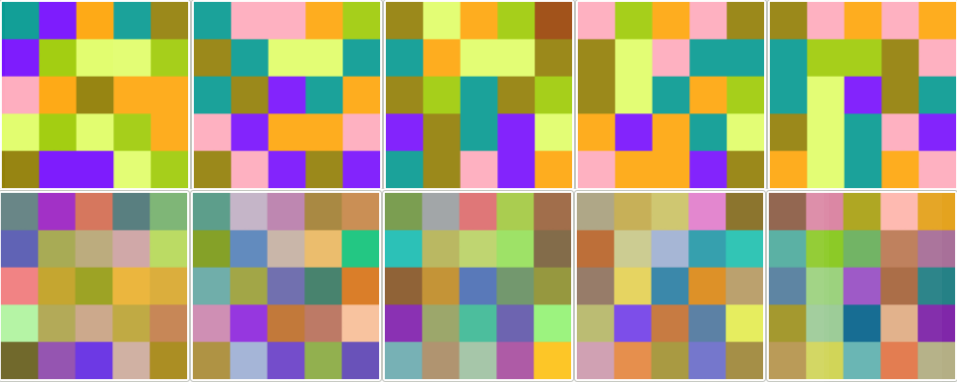
\includegraphics[width=0.8\textwidth]{images/generatedData__none_color_20_150_0_01_8_0_4_0_0_0_0_1_0_10_20___.png}
  \caption{ An example of SuperSquareShift noise, the top row is the true ground truth and the bottom row is the image data used for features with SuperSquareShift=0.4 included.  } 
  \label{fig:squareNoise}
\end{figure} 

\begin{figure}
  \centering
  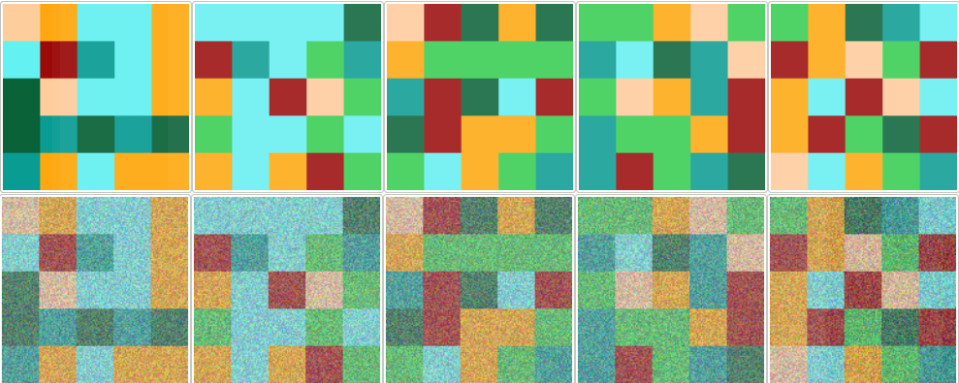
\includegraphics[width=0.8\textwidth]{images/generatedData__none_color_20_150_0_01_8_0_0_0_4_0_0_1_0_10_12___.png}
  \caption{ An example of WhiteNoise, the top row displays the groundtruth and the bottom are the feature images with whtieNoise=0.4 added. } 
  \label{fig:whiteNoise}
\end{figure} 

\begin{figure}
  \centering
  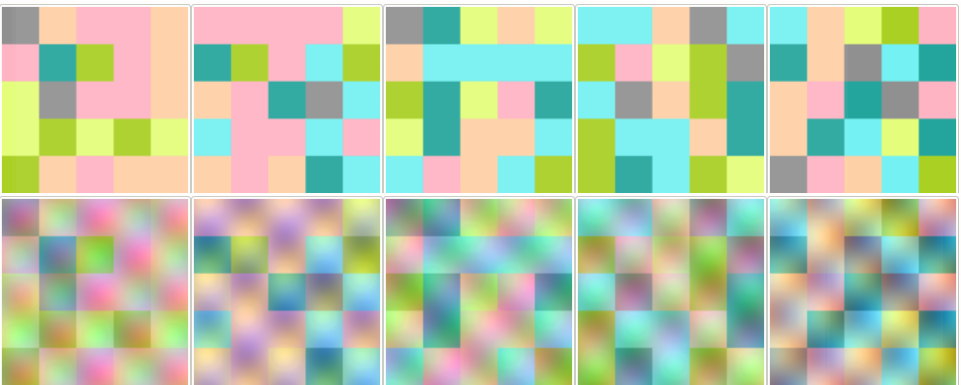
\includegraphics[width=0.8\textwidth]{images/generatedData__none_color_20_150_0_01_8_0_0_0_0_0_4_1_0_10_12___.png}
  \caption{ And example of OsilationNoise, the top row displays the groundtruth and the bottom row are the feature images with osilationNoise=0.4 added. } 
  \label{fig:osIlNoise}
\end{figure} 

\begin{figure}
  \centering
  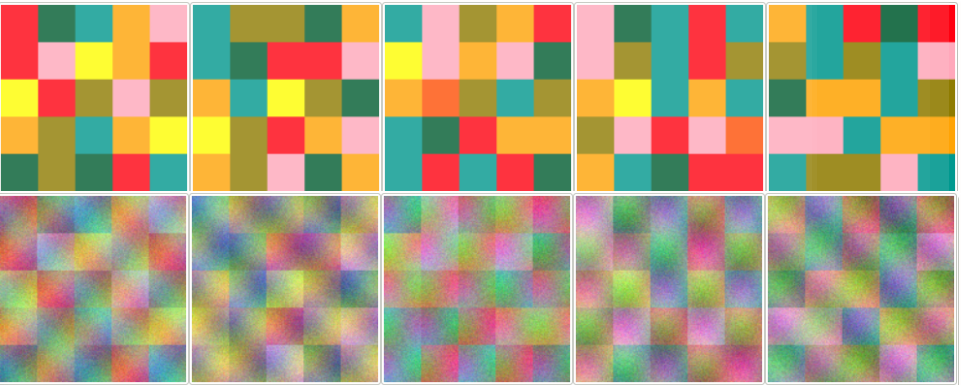
\includegraphics[width=0.8\textwidth]{images/generatedData__none_color_20_150_0_01_8_0_05_0_35_0_45_1_0_10_11___.png}
  \caption{  An example of all types of noise. The groundtruth is in the top row an the feature images are in the bottom row with the following nois added: Super-Square-shift=0.05, WhiteNoise=0.35 and OsilationNoise=0.45.} 
  \label{fig:allNoise}
\end{figure} 

\begin{figure}
  \centering
  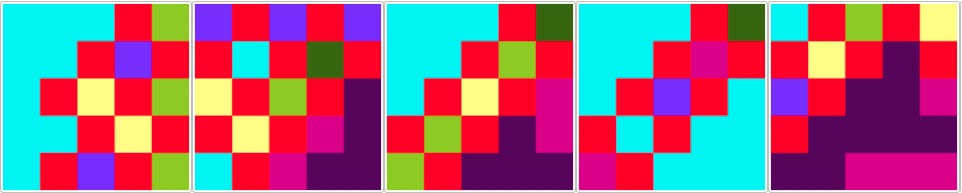
\includegraphics[width=0.8\textwidth]{images/DataGenNeighProb_0_3_seed13.png}
  \caption{  An example dataset showing groudataGenNeighProb=0.3, it can be contrasted to \ref{fig:allNoise} where the ground truth was generated with groudataGenNeighProb=1.0. We can see that in the above image some colors never occur next to each other.  } 
  \label{fig:dataGenNeighExp}
\end{figure} 


%


\backmatter

\bibliographystyle{plain}
\bibliography{refs}


\end{document}